%&preformat-disser
\RequirePackage[l2tabu,orthodox]{nag} % Раскомментировав, можно в логе получать рекомендации относительно правильного использования пакетов и предупреждения об устаревших и нерекомендуемых пакетах
% Формат А4, 14pt (ГОСТ Р 7.0.11-2011, 5.3.6)
\documentclass[a4paper,14pt,oneside,openany]{memoir}

\usepackage{eqexpl}
\eqexplSetIntro{где}
\eqexplSetItemWidth{7mm}
\eqexplSetDelim{--- }

%%%%%%%%%%%%%%%%%%%%%%%%%%%%%%%%%%%%%%%%%%%%%%%%%%%%%%%%%%%%%%%%%%%%%%%%%%%%%%%%
%%%% Файл упрощённых настроек шаблона, общих для диссертации и автореферата %%%%
%%%%%%%%%%%%%%%%%%%%%%%%%%%%%%%%%%%%%%%%%%%%%%%%%%%%%%%%%%%%%%%%%%%%%%%%%%%%%%%%

%%% Режим черновика %%%
\makeatletter
\@ifundefined{c@draft}{
  \newcounter{draft}
  \setcounter{draft}{0}  % 0 --- чистовик (максимальное соблюдение ГОСТ)
                         % 1 --- черновик (отклонения от ГОСТ, но быстрая
                         %       сборка итоговых PDF)
}{}
\makeatother

%%% Пометки в тексте %%%
\makeatletter
\@ifundefined{c@showmarkup}{
  \newcounter{showmarkup}
  \setcounter{showmarkup}{0}  % 0 --- скрыть пометки
                              % 1 --- показывать пометки
}{}
\makeatother

%%% Использование в pdflatex шрифтов не по-умолчанию %%%
\makeatletter
\@ifundefined{c@usealtfont}{
  \newcounter{usealtfont}
  \setcounter{usealtfont}{0}    % 0 --- шрифты на базе Computer Modern
                                % 1 --- использовать пакет pscyr, при его
                                %       наличии
                                % 2 --- использовать пакет XCharter, при наличии
                                %       подходящей версии
}{}
\makeatother

%%% Использование в xelatex и lualatex семейств шрифтов %%%
\makeatletter
\@ifundefined{c@fontfamily}{
  \newcounter{fontfamily}
  \setcounter{fontfamily}{0}  % 0 --- CMU семейство. Используется как fallback;
                              % 1 --- Шрифты от MS (Times New Roman и компания)
                              % 2 --- Семейство Liberation
}{}
\makeatother

%%% Библиография %%%
\makeatletter
\@ifundefined{c@bibliosel}{
  \newcounter{bibliosel}
  \setcounter{bibliosel}{1}   % 0 --- встроенная реализация с загрузкой файла
                              %       через движок bibtex8;
                              % 1 --- реализация пакетом biblatex через движок
                              %       biber
}{}
\makeatother

%%% Вывод типов ссылок в библиографии %%%
\makeatletter
\@ifundefined{c@mediadisplay}{
  \newcounter{mediadisplay}
  \setcounter{mediadisplay}{2}   % 0 --- не делать ничего; надписи [Текст] и
                                 %       [Эл. ресурс] будут выводиться только в ссылках с
                                 %       заполненным полем `media`;
                                 % 1 --- автоматически добавлять надпись [Текст] к ссылкам с
                                 %       незаполненным полем `media`; таким образом, у всех
                                 %       источников будет указан тип, что соответствует
                                 %       требованиям ГОСТ
                                 % 2 --- автоматически удалять надписи [Текст], [Эл. Ресурс] и др.;
                                 %       не соответствует ГОСТ
                                 % 3 --- автоматически удалять надпись [Текст];
                                 %       не соответствует ГОСТ
                                 % 4 --- автоматически удалять надпись [Эл. Ресурс];
                                 %       не соответствует ГОСТ
}{}
\makeatother

%%% Предкомпиляция tikz рисунков для ускорения работы %%%
\makeatletter
\@ifundefined{c@imgprecompile}{
  \newcounter{imgprecompile}
  \setcounter{imgprecompile}{0}   % 0 --- без предкомпиляции;
                                  % 1 --- пользоваться предварительно
                                  %       скомпилированными pdf вместо генерации
                                  %       заново из tikz
}{}
\makeatother
            % общие настройки шаблона
\input{common/packages}         % Пакеты общие для диссертации и автореферата
\synopsisfalse                      % Этот документ --- не автореферат
\input{Dissertation/dispackages}    % Пакеты для диссертации
\input{Dissertation/userpackages}   % Пакеты для специфических пользовательских задач

%%%%%%%%%%%%%%%%%%%%%%%%%%%%%%%%%%%%%%%%%%%%%%%%%%%%%%%%%%%%%%%%%%%%%%%%%%%%%%%%
%%%% Файл упрощённых настроек шаблона, общих для диссертации и автореферата %%%%
%%%%%%%%%%%%%%%%%%%%%%%%%%%%%%%%%%%%%%%%%%%%%%%%%%%%%%%%%%%%%%%%%%%%%%%%%%%%%%%%

%%% Режим черновика %%%
\makeatletter
\@ifundefined{c@draft}{
  \newcounter{draft}
  \setcounter{draft}{0}  % 0 --- чистовик (максимальное соблюдение ГОСТ)
                         % 1 --- черновик (отклонения от ГОСТ, но быстрая
                         %       сборка итоговых PDF)
}{}
\makeatother

%%% Пометки в тексте %%%
\makeatletter
\@ifundefined{c@showmarkup}{
  \newcounter{showmarkup}
  \setcounter{showmarkup}{0}  % 0 --- скрыть пометки
                              % 1 --- показывать пометки
}{}
\makeatother

%%% Использование в pdflatex шрифтов не по-умолчанию %%%
\makeatletter
\@ifundefined{c@usealtfont}{
  \newcounter{usealtfont}
  \setcounter{usealtfont}{0}    % 0 --- шрифты на базе Computer Modern
                                % 1 --- использовать пакет pscyr, при его
                                %       наличии
                                % 2 --- использовать пакет XCharter, при наличии
                                %       подходящей версии
}{}
\makeatother

%%% Использование в xelatex и lualatex семейств шрифтов %%%
\makeatletter
\@ifundefined{c@fontfamily}{
  \newcounter{fontfamily}
  \setcounter{fontfamily}{0}  % 0 --- CMU семейство. Используется как fallback;
                              % 1 --- Шрифты от MS (Times New Roman и компания)
                              % 2 --- Семейство Liberation
}{}
\makeatother

%%% Библиография %%%
\makeatletter
\@ifundefined{c@bibliosel}{
  \newcounter{bibliosel}
  \setcounter{bibliosel}{1}   % 0 --- встроенная реализация с загрузкой файла
                              %       через движок bibtex8;
                              % 1 --- реализация пакетом biblatex через движок
                              %       biber
}{}
\makeatother

%%% Вывод типов ссылок в библиографии %%%
\makeatletter
\@ifundefined{c@mediadisplay}{
  \newcounter{mediadisplay}
  \setcounter{mediadisplay}{2}   % 0 --- не делать ничего; надписи [Текст] и
                                 %       [Эл. ресурс] будут выводиться только в ссылках с
                                 %       заполненным полем `media`;
                                 % 1 --- автоматически добавлять надпись [Текст] к ссылкам с
                                 %       незаполненным полем `media`; таким образом, у всех
                                 %       источников будет указан тип, что соответствует
                                 %       требованиям ГОСТ
                                 % 2 --- автоматически удалять надписи [Текст], [Эл. Ресурс] и др.;
                                 %       не соответствует ГОСТ
                                 % 3 --- автоматически удалять надпись [Текст];
                                 %       не соответствует ГОСТ
                                 % 4 --- автоматически удалять надпись [Эл. Ресурс];
                                 %       не соответствует ГОСТ
}{}
\makeatother

%%% Предкомпиляция tikz рисунков для ускорения работы %%%
\makeatletter
\@ifundefined{c@imgprecompile}{
  \newcounter{imgprecompile}
  \setcounter{imgprecompile}{0}   % 0 --- без предкомпиляции;
                                  % 1 --- пользоваться предварительно
                                  %       скомпилированными pdf вместо генерации
                                  %       заново из tikz
}{}
\makeatother
      % Упрощённые настройки шаблона

\input{common/newnames}         % Новые переменные, для всего проекта

%%% Основные сведения %%%
\newcommand{\thesisAuthorLastName}{\fixme{Фурашов}}
\newcommand{\thesisAuthorOtherNames}{\fixme{Александр Станиславович}}
\newcommand{\thesisAuthorInitials}{\fixme{А.\,С.}}
\newcommand{\thesisAuthor}             % Диссертация, ФИО автора
{%
    \texorpdfstring{% \texorpdfstring takes two arguments and uses the first for (La)TeX and the second for pdf
        \thesisAuthorLastName~\thesisAuthorOtherNames% так будет отображаться на титульном листе или в тексте, где будет использоваться переменная
    }{%
        \thesisAuthorLastName, \thesisAuthorOtherNames% эта запись для свойств pdf-файла. В таком виде, если pdf будет обработан программами для сбора библиографических сведений, будет правильно представлена фамилия.
    }
}
\newcommand{\thesisAuthorShort}        % Диссертация, ФИО автора инициалами
{\thesisAuthorInitials~\thesisAuthorLastName}
\newcommand{\thesisUdk}                % Диссертация, УДК
{\fixme{621.634}}
\newcommand{\thesisTitle}              % Диссертация, название
{\fixme{Усовершеноствованный метод проектирования высоконапорного вентилятора с меридиональным ускорением потока}}
\newcommand{\thesisSpecialtyNumber}    % Диссертация, специальность, номер
{\fixme{2.4.7.}}
\newcommand{\thesisSpecialtyTitle}     % Диссертация, специальность, название (название взято с сайта ВАК для примера)
{\fixme{Турбомашины и поршневые двигатели}}
%% \newcommand{\thesisSpecialtyTwoNumber} % Диссертация, вторая специальность, номер
%% {\fixme{XX.XX.XX}}
%% \newcommand{\thesisSpecialtyTwoTitle}  % Диссертация, вторая специальность, название
%% {\fixme{Теория и~методика физического воспитания, спортивной тренировки,
%% оздоровительной и~адаптивной физической культуры}}
\newcommand{\thesisDegree}             % Диссертация, ученая степень
{\fixme{кандидата технических наук}}
\newcommand{\thesisDegreeShort}        % Диссертация, ученая степень, краткая запись
{\fixme{канд. техн. наук}}
\newcommand{\thesisCity}               % Диссертация, город написания диссертации
{\fixme{Москва}}
\newcommand{\thesisYear}               % Диссертация, год написания диссертации
{\the\year}
\newcommand{\thesisOrganization}       % Диссертация, организация
{\fixme{федеральное государственное бюджетное образовательное учреждение высшего образования <<Московский государственный технический университет имени Н.\,Э.\,Баумана (национальный исследовательский университет)>>}}
\newcommand{\thesisOrganizationShort}  % Диссертация, краткое название организации для доклада
{\fixme{МГТУ им.~Н.\,Э.~Баумана}}

\newcommand{\thesisInOrganization}     % Диссертация, организация в предложном падеже: Работа выполнена в ...
{\fixme{ФАУ <<ЦАГИ>>}}

%% \newcommand{\supervisorDead}{}           % Рисовать рамку вокруг фамилии
\newcommand{\supervisorFio}              % Научный руководитель, ФИО
{\fixme{Арбеков Александр Николаевич}}
\newcommand{\supervisorRegalia}          % Научный руководитель, регалии
{\fixme{доктор технических наук, доцент}}
\newcommand{\supervisorFioShort}         % Научный руководитель, ФИО
{\fixme{А.\,Н.~Арбеков}}
\newcommand{\supervisorRegaliaShort}     % Научный руководитель, регалии
{\fixme{д-р техн. наук,~ доц.}}

%% \newcommand{\supervisorTwoDead}{}        % Рисовать рамку вокруг фамилии
%% \newcommand{\supervisorTwoFio}           % Второй научный руководитель, ФИО
%% {\fixme{Фамилия Имя Отчество}}
%% \newcommand{\supervisorTwoRegalia}       % Второй научный руководитель, регалии
%% {\fixme{уч. степень, уч. звание}}
%% \newcommand{\supervisorTwoFioShort}      % Второй научный руководитель, ФИО
%% {\fixme{И.\,О.~Фамилия}}
%% \newcommand{\supervisorTwoRegaliaShort}  % Второй научный руководитель, регалии
%% {\fixme{уч.~ст.,~уч.~зв.}}

\newcommand{\opponentOneFio}           % Оппонент 1, ФИО
{\fixme{Фамилия Имя Отчество}}
\newcommand{\opponentOneRegalia}       % Оппонент 1, регалии
{\fixme{доктор физико-математических наук, профессор}}
\newcommand{\opponentOneJobPlace}      % Оппонент 1, место работы
{\fixme{Не очень длинное название для места работы}}
\newcommand{\opponentOneJobPost}       % Оппонент 1, должность
{\fixme{старший научный сотрудник}}

\newcommand{\opponentTwoFio}           % Оппонент 2, ФИО
{\fixme{Фамилия Имя Отчество}}
\newcommand{\opponentTwoRegalia}       % Оппонент 2, регалии
{\fixme{кандидат физико-математических наук}}
\newcommand{\opponentTwoJobPlace}      % Оппонент 2, место работы
{\fixme{Основное место работы c длинным длинным длинным длинным названием}}
\newcommand{\opponentTwoJobPost}       % Оппонент 2, должность
{\fixme{старший научный сотрудник}}

%% \newcommand{\opponentThreeFio}         % Оппонент 3, ФИО
%% {\fixme{Фамилия Имя Отчество}}
%% \newcommand{\opponentThreeRegalia}     % Оппонент 3, регалии
%% {\fixme{кандидат физико-математических наук}}
%% \newcommand{\opponentThreeJobPlace}    % Оппонент 3, место работы
%% {\fixme{Основное место работы c длинным длинным длинным длинным названием}}
%% \newcommand{\opponentThreeJobPost}     % Оппонент 3, должность
%% {\fixme{старший научный сотрудник}}

\newcommand{\leadingOrganizationTitle} % Ведущая организация, дополнительные строки. Удалить, чтобы не отображать в автореферате
{\fixme{Федеральное государственное бюджетное образовательное учреждение высшего
профессионального образования с~длинным длинным длинным длинным названием}}

\newcommand{\defenseDate}              % Защита, дата
{\fixme{DD mmmmmmmm YYYY~г.~в~XX часов}}
\newcommand{\defenseCouncilNumber}     % Защита, номер диссертационного совета
{\fixme{Д\,123.456.78}}
\newcommand{\defenseCouncilTitle}      % Защита, учреждение диссертационного совета
{\fixme{Название учреждения}}
\newcommand{\defenseCouncilAddress}    % Защита, адрес учреждение диссертационного совета
{\fixme{Адрес}}
\newcommand{\defenseCouncilPhone}      % Телефон для справок
{\fixme{+7~(0000)~00-00-00}}

\newcommand{\defenseSecretaryFio}      % Секретарь диссертационного совета, ФИО
{\fixme{Фамилия Имя Отчество}}
\newcommand{\defenseSecretaryRegalia}  % Секретарь диссертационного совета, регалии
{\fixme{д-р~физ.-мат. наук}}            % Для сокращений есть ГОСТы, например: ГОСТ Р 7.0.12-2011 + http://base.garant.ru/179724/#block_30000

\newcommand{\synopsisLibrary}          % Автореферат, название библиотеки
{\fixme{Название библиотеки}}
\newcommand{\synopsisDate}             % Автореферат, дата рассылки
{\fixme{DD mmmmmmmm}\the\year~года}

% To avoid conflict with beamer class use \providecommand
\providecommand{\keywords}%            % Ключевые слова для метаданных PDF диссертации и автореферата
{}

             % Основные сведения
\input{common/fonts}            % Определение шрифтов (частичное)
%%% Шаблон %%%
\DeclareRobustCommand{\fixme}{\textcolor{black}}  % решаем проблему превращения
                                % названия цвета в результате \MakeUppercase,
                                % http://tex.stackexchange.com/a/187930,
                                % \DeclareRobustCommand protects \fixme
                                % from expanding inside \MakeUppercase
\AtBeginDocument{%
    \setlength{\parindent}{2.5em}                   % Абзацный отступ. Должен быть одинаковым по всему тексту и равен пяти знакам (ГОСТ Р 7.0.11-2011, 5.3.7).
}

%%% Таблицы %%%
\DeclareCaptionLabelSeparator{tabsep}{\tablabelsep} % нумерация таблиц
\DeclareCaptionFormat{split}{\splitformatlabel#1\par\splitformattext#3}

\captionsetup[table]{
        format=\tabformat,                % формат подписи (plain|hang)
        font=normal,                      % нормальные размер, цвет, стиль шрифта
        skip=.0pt,                        % отбивка под подписью
        parskip=.0pt,                     % отбивка между параграфами подписи
        position=above,                   % положение подписи
        justification=\tabjust,           % центровка
        indent=\tabindent,                % смещение строк после первой
        labelsep=tabsep,                  % разделитель
        singlelinecheck=\tabsinglecenter, % не выравнивать по центру, если умещается в одну строку
}

%%% Рисунки %%%
\DeclareCaptionLabelSeparator{figsep}{\figlabelsep} % нумерация рисунков

\captionsetup[figure]{
        format=plain,                     % формат подписи (plain|hang)
        font=normal,                      % нормальные размер, цвет, стиль шрифта
        skip=.0pt,                        % отбивка под подписью
        parskip=.0pt,                     % отбивка между параграфами подписи
        position=below,                   % положение подписи
        singlelinecheck=true,             % выравнивание по центру, если умещается в одну строку
        justification=centerlast,         % центровка
        labelsep=figsep,                  % разделитель
}

%%% Подписи подрисунков %%%
\DeclareCaptionSubType{figure}
\renewcommand\thesubfigure{\asbuk{subfigure}} % нумерация подрисунков
\ifsynopsis
\DeclareCaptionFont{norm}{\fontsize{10pt}{11pt}\selectfont}
\newcommand{\subfigureskip}{2.pt}
\else
\DeclareCaptionFont{norm}{\fontsize{14pt}{16pt}\selectfont}
\newcommand{\subfigureskip}{0.pt}
\fi

\captionsetup[subfloat]{
        labelfont=norm,                 % нормальный размер подписей подрисунков
        textfont=norm,                  % нормальный размер подписей подрисунков
        labelsep=space,                 % разделитель
        labelformat=brace,              % одна скобка справа от номера
        justification=centering,        % центровка
        singlelinecheck=true,           % выравнивание по центру, если умещается в одну строку
        skip=\subfigureskip,            % отбивка над подписью
        parskip=.0pt,                   % отбивка между параграфами подписи
        position=below,                 % положение подписи
}

%%% Настройки ссылок на рисунки, таблицы и др. %%%
% команды \cref...format отвечают за форматирование при помощи команды \cref
% команды \labelcref...format отвечают за форматирование при помощи команды \labelcref

\ifpresentation
\else
    \crefdefaultlabelformat{#2#1#3}

    % Уравнение
    \crefformat{equation}{(#2#1#3)} % одиночная ссылка с приставкой
    \labelcrefformat{equation}{(#2#1#3)} % одиночная ссылка без приставки
    \crefrangeformat{equation}{(#3#1#4) \cyrdash~(#5#2#6)} % диапазон ссылок с приставкой
    \labelcrefrangeformat{equation}{(#3#1#4) \cyrdash~(#5#2#6)} % диапазон ссылок без приставки
    \crefmultiformat{equation}{(#2#1#3)}{ и~(#2#1#3)}{, (#2#1#3)}{ и~(#2#1#3)} % перечисление ссылок с приставкой
    \labelcrefmultiformat{equation}{(#2#1#3)}{ и~(#2#1#3)}{, (#2#1#3)}{ и~(#2#1#3)} % перечисление без приставки

    % Подуравнение
    \crefformat{subequation}{(#2#1#3)} % одиночная ссылка с приставкой
    \labelcrefformat{subequation}{(#2#1#3)} % одиночная ссылка без приставки
    \crefrangeformat{subequation}{(#3#1#4) \cyrdash~(#5#2#6)} % диапазон ссылок с приставкой
    \labelcrefrangeformat{subequation}{(#3#1#4) \cyrdash~(#5#2#6)} % диапазон ссылок без приставки
    \crefmultiformat{subequation}{(#2#1#3)}{ и~(#2#1#3)}{, (#2#1#3)}{ и~(#2#1#3)} % перечисление ссылок с приставкой
    \labelcrefmultiformat{subequation}{(#2#1#3)}{ и~(#2#1#3)}{, (#2#1#3)}{ и~(#2#1#3)} % перечисление без приставки

    % Глава
    \crefformat{chapter}{#2#1#3} % одиночная ссылка с приставкой
    \labelcrefformat{chapter}{#2#1#3} % одиночная ссылка без приставки
    \crefrangeformat{chapter}{#3#1#4 \cyrdash~#5#2#6} % диапазон ссылок с приставкой
    \labelcrefrangeformat{chapter}{#3#1#4 \cyrdash~#5#2#6} % диапазон ссылок без приставки
    \crefmultiformat{chapter}{#2#1#3}{ и~#2#1#3}{, #2#1#3}{ и~#2#1#3} % перечисление ссылок с приставкой
    \labelcrefmultiformat{chapter}{#2#1#3}{ и~#2#1#3}{, #2#1#3}{ и~#2#1#3} % перечисление без приставки

    % Параграф
    \crefformat{section}{#2#1#3} % одиночная ссылка с приставкой
    \labelcrefformat{section}{#2#1#3} % одиночная ссылка без приставки
    \crefrangeformat{section}{#3#1#4 \cyrdash~#5#2#6} % диапазон ссылок с приставкой
    \labelcrefrangeformat{section}{#3#1#4 \cyrdash~#5#2#6} % диапазон ссылок без приставки
    \crefmultiformat{section}{#2#1#3}{ и~#2#1#3}{, #2#1#3}{ и~#2#1#3} % перечисление ссылок с приставкой
    \labelcrefmultiformat{section}{#2#1#3}{ и~#2#1#3}{, #2#1#3}{ и~#2#1#3} % перечисление без приставки

    % Приложение
    \crefformat{appendix}{#2#1#3} % одиночная ссылка с приставкой
    \labelcrefformat{appendix}{#2#1#3} % одиночная ссылка без приставки
    \crefrangeformat{appendix}{#3#1#4 \cyrdash~#5#2#6} % диапазон ссылок с приставкой
    \labelcrefrangeformat{appendix}{#3#1#4 \cyrdash~#5#2#6} % диапазон ссылок без приставки
    \crefmultiformat{appendix}{#2#1#3}{ и~#2#1#3}{, #2#1#3}{ и~#2#1#3} % перечисление ссылок с приставкой
    \labelcrefmultiformat{appendix}{#2#1#3}{ и~#2#1#3}{, #2#1#3}{ и~#2#1#3} % перечисление без приставки

    % Рисунок
    \crefformat{figure}{#2#1#3} % одиночная ссылка с приставкой
    \labelcrefformat{figure}{#2#1#3} % одиночная ссылка без приставки
    \crefrangeformat{figure}{#3#1#4 \cyrdash~#5#2#6} % диапазон ссылок с приставкой
    \labelcrefrangeformat{figure}{#3#1#4 \cyrdash~#5#2#6} % диапазон ссылок без приставки
    \crefmultiformat{figure}{#2#1#3}{ и~#2#1#3}{, #2#1#3}{ и~#2#1#3} % перечисление ссылок с приставкой
    \labelcrefmultiformat{figure}{#2#1#3}{ и~#2#1#3}{, #2#1#3}{ и~#2#1#3} % перечисление без приставки

    % Таблица
    \crefformat{table}{#2#1#3} % одиночная ссылка с приставкой
    \labelcrefformat{table}{#2#1#3} % одиночная ссылка без приставки
    \crefrangeformat{table}{#3#1#4 \cyrdash~#5#2#6} % диапазон ссылок с приставкой
    \labelcrefrangeformat{table}{#3#1#4 \cyrdash~#5#2#6} % диапазон ссылок без приставки
    \crefmultiformat{table}{#2#1#3}{ и~#2#1#3}{, #2#1#3}{ и~#2#1#3} % перечисление ссылок с приставкой
    \labelcrefmultiformat{table}{#2#1#3}{ и~#2#1#3}{, #2#1#3}{ и~#2#1#3} % перечисление без приставки

    % Листинг
    \crefformat{lstlisting}{#2#1#3} % одиночная ссылка с приставкой
    \labelcrefformat{lstlisting}{#2#1#3} % одиночная ссылка без приставки
    \crefrangeformat{lstlisting}{#3#1#4 \cyrdash~#5#2#6} % диапазон ссылок с приставкой
    \labelcrefrangeformat{lstlisting}{#3#1#4 \cyrdash~#5#2#6} % диапазон ссылок без приставки
    \crefmultiformat{lstlisting}{#2#1#3}{ и~#2#1#3}{, #2#1#3}{ и~#2#1#3} % перечисление ссылок с приставкой
    \labelcrefmultiformat{lstlisting}{#2#1#3}{ и~#2#1#3}{, #2#1#3}{ и~#2#1#3} % перечисление без приставки

    % Листинг
    \crefformat{ListingEnv}{#2#1#3} % одиночная ссылка с приставкой
    \labelcrefformat{ListingEnv}{#2#1#3} % одиночная ссылка без приставки
    \crefrangeformat{ListingEnv}{#3#1#4 \cyrdash~#5#2#6} % диапазон ссылок с приставкой
    \labelcrefrangeformat{ListingEnv}{#3#1#4 \cyrdash~#5#2#6} % диапазон ссылок без приставки
    \crefmultiformat{ListingEnv}{#2#1#3}{ и~#2#1#3}{, #2#1#3}{ и~#2#1#3} % перечисление ссылок с приставкой
    \labelcrefmultiformat{ListingEnv}{#2#1#3}{ и~#2#1#3}{, #2#1#3}{ и~#2#1#3} % перечисление без приставки
\fi

%%% Настройки гиперссылок %%%
\ifluatex
    \hypersetup{
        unicode,                % Unicode encoded PDF strings
    }
\fi

\hypersetup{
    linktocpage=true,           % ссылки с номера страницы в оглавлении, списке таблиц и списке рисунков
%    linktoc=all,                % both the section and page part are links
%    pdfpagelabels=false,        % set PDF page labels (true|false)
    plainpages=false,           % Forces page anchors to be named by the Arabic form  of the page number, rather than the formatted form
    colorlinks,                 % ссылки отображаются раскрашенным текстом, а не раскрашенным прямоугольником, вокруг текста
    linkcolor={linkcolor},      % цвет ссылок типа ref, eqref и подобных
    citecolor={citecolor},      % цвет ссылок-цитат
    urlcolor={urlcolor},        % цвет гиперссылок
%    hidelinks,                  % Hide links (removing color and border)
    pdftitle={\thesisTitle},    % Заголовок
    pdfauthor={\thesisAuthor},  % Автор
    pdfsubject={\thesisSpecialtyNumber\ \thesisSpecialtyTitle},      % Тема
%    pdfcreator={Создатель},     % Создатель, Приложение
%    pdfproducer={Производитель},% Производитель, Производитель PDF
    pdfkeywords={\keywords},    % Ключевые слова
    pdflang={ru},
}
\ifnumequal{\value{draft}}{1}{% Черновик
    \hypersetup{
        draft,
    }
}{}

%%% Списки %%%
% Используем короткое тире (endash) для ненумерованных списков (ГОСТ 2.105-95, пункт 4.1.7, требует дефиса, но так лучше смотрится)
\renewcommand{\labelitemi}{\normalfont\bfseries{--}}

% Перечисление строчными буквами латинского алфавита (ГОСТ 2.105-95, 4.1.7)
%\renewcommand{\theenumi}{\alph{enumi}}
%\renewcommand{\labelenumi}{\theenumi)}

% Перечисление строчными буквами русского алфавита (ГОСТ 2.105-95, 4.1.7)
\makeatletter
\AddEnumerateCounter{\asbuk}{\russian@alph}{щ}      % Управляем списками/перечислениями через пакет enumitem, а он 'не знает' про asbuk, потому 'учим' его
\makeatother
%\renewcommand{\theenumi}{\asbuk{enumi}} %первый уровень нумерации
%\renewcommand{\labelenumi}{\theenumi)} %первый уровень нумерации
\renewcommand{\theenumii}{\asbuk{enumii}} %второй уровень нумерации
\renewcommand{\labelenumii}{\theenumii)} %второй уровень нумерации
\renewcommand{\theenumiii}{\arabic{enumiii}} %третий уровень нумерации
\renewcommand{\labelenumiii}{\theenumiii)} %третий уровень нумерации

\setlist{nosep,%                                    % Единый стиль для всех списков (пакет enumitem), без дополнительных интервалов.
    labelindent=\parindent,leftmargin=*%            % Каждый пункт, подпункт и перечисление записывают с абзацного отступа (ГОСТ 2.105-95, 4.1.8)
}

%%% Правильная нумерация приложений, рисунков и формул %%%
%% По ГОСТ 2.105, п. 4.3.8 Приложения обозначают заглавными буквами русского алфавита,
%% начиная с А, за исключением букв Ё, З, Й, О, Ч, Ь, Ы, Ъ.
%% Здесь также переделаны все нумерации русскими буквами.
\ifxetexorluatex
    \makeatletter
    \def\russian@Alph#1{\ifcase#1\or
       А\or Б\or В\or Г\or Д\or Е\or Ж\or
       И\or К\or Л\or М\or Н\or
       П\or Р\or С\or Т\or У\or Ф\or Х\or
       Ц\or Ш\or Щ\or Э\or Ю\or Я\else\xpg@ill@value{#1}{russian@Alph}\fi}
    \def\russian@alph#1{\ifcase#1\or
       а\or б\or в\or г\or д\or е\or ж\or
       и\or к\or л\or м\or н\or
       п\or р\or с\or т\or у\or ф\or х\or
       ц\or ш\or щ\or э\or ю\or я\else\xpg@ill@value{#1}{russian@alph}\fi}
    \def\cyr@Alph#1{\ifcase#1\or
        А\or Б\or В\or Г\or Д\or Е\or Ж\or
        И\or К\or Л\or М\or Н\or
        П\or Р\or С\or Т\or У\or Ф\or Х\or
        Ц\or Ш\or Щ\or Э\or Ю\or Я\else\xpg@ill@value{#1}{cyr@Alph}\fi}
    \def\cyr@alph#1{\ifcase#1\or
        а\or б\or в\or г\or д\or е\or ж\or
        и\or к\or л\or м\or н\or
        п\or р\or с\or т\or у\or ф\or х\or
        ц\or ш\or щ\or э\or ю\or я\else\xpg@ill@value{#1}{cyr@alph}\fi}
    \makeatother
\else
    \makeatletter
    \if@uni@ode
      \def\russian@Alph#1{\ifcase#1\or
        А\or Б\or В\or Г\or Д\or Е\or Ж\or
        И\or К\or Л\or М\or Н\or
        П\or Р\or С\or Т\or У\or Ф\or Х\or
        Ц\or Ш\or Щ\or Э\or Ю\or Я\else\@ctrerr\fi}
    \else
      \def\russian@Alph#1{\ifcase#1\or
        \CYRA\or\CYRB\or\CYRV\or\CYRG\or\CYRD\or\CYRE\or\CYRZH\or
        \CYRI\or\CYRK\or\CYRL\or\CYRM\or\CYRN\or
        \CYRP\or\CYRR\or\CYRS\or\CYRT\or\CYRU\or\CYRF\or\CYRH\or
        \CYRC\or\CYRSH\or\CYRSHCH\or\CYREREV\or\CYRYU\or
        \CYRYA\else\@ctrerr\fi}
    \fi
    \if@uni@ode
      \def\russian@alph#1{\ifcase#1\or
        а\or б\or в\or г\or д\or е\or ж\or
        и\or к\or л\or м\or н\or
        п\or р\or с\or т\or у\or ф\or х\or
        ц\or ш\or щ\or э\or ю\or я\else\@ctrerr\fi}
    \else
      \def\russian@alph#1{\ifcase#1\or
        \cyra\or\cyrb\or\cyrv\or\cyrg\or\cyrd\or\cyre\or\cyrzh\or
        \cyri\or\cyrk\or\cyrl\or\cyrm\or\cyrn\or
        \cyrp\or\cyrr\or\cyrs\or\cyrt\or\cyru\or\cyrf\or\cyrh\or
        \cyrc\or\cyrsh\or\cyrshch\or\cyrerev\or\cyryu\or
        \cyrya\else\@ctrerr\fi}
    \fi
    \makeatother
\fi


%%http://www.linux.org.ru/forum/general/6993203#comment-6994589 (используется totcount)
\makeatletter
\def\formtotal#1#2#3#4#5{%
    \newcount\@c
    \@c\totvalue{#1}\relax
    \newcount\@last
    \newcount\@pnul
    \@last\@c\relax
    \divide\@last 10
    \@pnul\@last\relax
    \divide\@pnul 10
    \multiply\@pnul-10
    \advance\@pnul\@last
    \multiply\@last-10
    \advance\@last\@c
    #2%
    \ifnum\@pnul=1#5\else%
    \ifcase\@last#5\or#3\or#4\or#4\or#4\else#5\fi
    \fi
}
\makeatother

\newcommand{\formbytotal}[5]{\total{#1}~\formtotal{#1}{#2}{#3}{#4}{#5}}

%%% Команды рецензирования %%%
\ifboolexpr{ (test {\ifnumequal{\value{draft}}{1}}) or (test {\ifnumequal{\value{showmarkup}}{1}})}{
        \newrobustcmd{\todo}[1]{\textcolor{red}{#1}}
        \newrobustcmd{\note}[2][]{\ifstrempty{#1}{#2}{\textcolor{#1}{#2}}}
        \newenvironment{commentbox}[1][]%
        {\ifstrempty{#1}{}{\color{#1}}}%
        {}
}{
        \newrobustcmd{\todo}[1]{}
        \newrobustcmd{\note}[2][]{}
        \excludecomment{commentbox}
}
           % Стили общие для диссертации и автореферата
%%% Переопределение именований, если иначе не сработает %%%
%\gappto\captionsrussian{
%    \renewcommand{\chaptername}{Глава}
%    \renewcommand{\appendixname}{Приложение} % (ГОСТ Р 7.0.11-2011, 5.7)
%}

%%% Изображения %%%
\graphicspath{{images/}{Dissertation/images/}}         % Пути к изображениям

%%% Интервалы %%%
%% По ГОСТ Р 7.0.11-2011, пункту 5.3.6 требуется полуторный интервал
%% Реализация средствами класса (на основе setspace) ближе к типографской классике.
%% И правит сразу и в таблицах (если со звёздочкой)
%\DoubleSpacing*     % Двойной интервал
\OnehalfSpacing*    % Полуторный интервал
%\setSpacing{1.42}   % Полуторный интервал, подобный Ворду (возможно, стоит включать вместе с предыдущей строкой)

%%% Макет страницы %%%
% Выставляем значения полей (ГОСТ 7.0.11-2011, 5.3.7)
\geometry{a4paper, top=2cm, bottom=2cm, left=2.5cm, right=1cm, nofoot, nomarginpar} %, heightrounded, showframe
%\geometry{a5paper, top=0.5cm, bottom=0.5cm, left=0.5cm, right=0.5cm, nofoot, nomarginpar}
\setlength{\topskip}{0pt}   %размер дополнительного верхнего поля
\setlength{\footskip}{12.3pt} % снимет warning, согласно https://tex.stackexchange.com/a/334346

%%% Выравнивание и переносы %%%
%% http://tex.stackexchange.com/questions/241343/what-is-the-meaning-of-fussy-sloppy-emergencystretch-tolerance-hbadness
%% http://www.latex-community.org/forum/viewtopic.php?p=70342#p70342
\tolerance 1414
\hbadness 1414
\emergencystretch 1.5em % В случае проблем регулировать в первую очередь
\hfuzz 0.3pt
\vfuzz \hfuzz
%\raggedbottom
%\sloppy                 % Избавляемся от переполнений
\clubpenalty=10000      % Запрещаем разрыв страницы после первой строки абзаца
\widowpenalty=10000     % Запрещаем разрыв страницы после последней строки абзаца
\brokenpenalty=4991     % Ограничение на разрыв страницы, если строка заканчивается переносом

%%% Блок управления параметрами для выравнивания заголовков в тексте %%%
\newlength{\otstuplen}
\setlength{\otstuplen}{\theotstup\parindent}
\ifnumequal{\value{headingalign}}{0}{% выравнивание заголовков в тексте
    \newcommand{\hdngalign}{\centering}                % по центру
    \newcommand{\hdngaligni}{}% по центру
    \setlength{\otstuplen}{0pt}
}{%
    \newcommand{\hdngalign}{}                 % по левому краю
    \newcommand{\hdngaligni}{\hspace{\otstuplen}}      % по левому краю
} % В обоих случаях вроде бы без переноса, как и надо (ГОСТ Р 7.0.11-2011, 5.3.5)

%%% Оглавление %%%
\renewcommand{\cftchapterdotsep}{\cftdotsep}                % отбивка точками до номера страницы начала главы/раздела

%% Переносить слова в заголовке не допускается (ГОСТ Р 7.0.11-2011, 5.3.5). Заголовки в оглавлении должны точно повторять заголовки в тексте (ГОСТ Р 7.0.11-2011, 5.2.3). Прямого указания на запрет переносов в оглавлении нет, но по той же логике невнесения искажений в смысл, лучше в оглавлении не переносить:
\setrmarg{2.55em plus1fil}                             %To have the (sectional) titles in the ToC, etc., typeset ragged right with no hyphenation
\renewcommand{\cftchapterpagefont}{\normalfont}        % нежирные номера страниц у глав в оглавлении
\renewcommand{\cftchapterleader}{\cftdotfill{\cftchapterdotsep}}% нежирные точки до номеров страниц у глав в оглавлении
%\renewcommand{\cftchapterfont}{}                       % нежирные названия глав в оглавлении

\ifnumgreater{\value{headingdelim}}{0}{%
    \renewcommand\cftchapteraftersnum{.\space}       % добавляет точку с пробелом после номера раздела в оглавлении
}{}
\ifnumgreater{\value{headingdelim}}{1}{%
    \renewcommand\cftsectionaftersnum{.\space}       % добавляет точку с пробелом после номера подраздела в оглавлении
    \renewcommand\cftsubsectionaftersnum{.\space}    % добавляет точку с пробелом после номера подподраздела в оглавлении
    \renewcommand\cftsubsubsectionaftersnum{.\space} % добавляет точку с пробелом после номера подподподраздела в оглавлении
    \AfterEndPreamble{% без этого polyglossia сама всё переопределяет
        \setsecnumformat{\csname the#1\endcsname.\space}
    }
}{%
    \AfterEndPreamble{% без этого polyglossia сама всё переопределяет
        \setsecnumformat{\csname the#1\endcsname\quad}
    }
}

\renewcommand*{\cftappendixname}{\appendixname\space} % Слово Приложение в оглавлении

%%% Колонтитулы %%%
% Порядковый номер страницы печатают на середине верхнего поля страницы (ГОСТ Р 7.0.11-2011, 5.3.8)
\makeevenhead{plain}{}{\rmfamily\thepage}{}
\makeoddhead{plain}{}{\rmfamily\thepage}{}
\makeevenfoot{plain}{}{}{}
\makeoddfoot{plain}{}{}{}
\pagestyle{plain}

%%% добавить Стр. над номерами страниц в оглавлении
%%% http://tex.stackexchange.com/a/306950
\newif\ifendTOC

\newcommand*{\tocheader}{
\ifnumequal{\value{pgnum}}{1}{%
    \ifendTOC\else\hbox to \linewidth%
      {\noindent{}~\hfill{Стр.}}\par%
      \ifnumless{\value{page}}{3}{}{%
        \vspace{0.5\onelineskip}
      }
      \afterpage{\tocheader}
    \fi%
}{}%
}%

%%% Оформление заголовков глав, разделов, подразделов %%%
%% Работа должна быть выполнена ... размером шрифта 12-14 пунктов (ГОСТ Р 7.0.11-2011, 5.3.8). То есть не должно быть надписей шрифтом более 14. Так и поставим.
%% Эти установки будут давать одинаковый результат независимо от выбора базовым шрифтом 12 пт или 14 пт
\newcommand{\basegostsectionfont}{\fontsize{14pt}{16pt}\selectfont\bfseries}

\makechapterstyle{thesisgost}{%
    \chapterstyle{default}
    \setlength{\beforechapskip}{0pt}
    \setlength{\midchapskip}{0pt}
    \setlength{\afterchapskip}{\theintvl\curtextsize}
    \renewcommand*{\chapnamefont}{\basegostsectionfont}
    \renewcommand*{\chapnumfont}{\basegostsectionfont}
    \renewcommand*{\chaptitlefont}{\basegostsectionfont}
    \renewcommand*{\chapterheadstart}{}
    \ifnumgreater{\value{headingdelim}}{0}{%
        \renewcommand*{\afterchapternum}{.\space}   % добавляет точку с пробелом после номера раздела
    }{%
        \renewcommand*{\afterchapternum}{\quad}     % добавляет \quad после номера раздела
    }
    \renewcommand*{\printchapternum}{\hdngaligni\hdngalign\chapnumfont \thechapter}
    \renewcommand*{\printchaptername}{}
    \renewcommand*{\printchapternonum}{\hdngaligni\hdngalign}
}

\makeatletter
\makechapterstyle{thesisgostchapname}{%
    \chapterstyle{thesisgost}
    \renewcommand*{\printchapternum}{\chapnumfont \thechapter}
    \renewcommand*{\printchaptername}{\hdngaligni\hdngalign\chapnamefont \@chapapp} %
}
\makeatother

\chapterstyle{thesisgost}

\setsecheadstyle{\basegostsectionfont\hdngalign}
\setsecindent{\otstuplen}

\setsubsecheadstyle{\basegostsectionfont\hdngalign}
\setsubsecindent{\otstuplen}

\setsubsubsecheadstyle{\basegostsectionfont\hdngalign}
\setsubsubsecindent{\otstuplen}

\sethangfrom{\noindent #1} %все заголовки подразделов центрируются с учетом номера, как block

\ifnumequal{\value{chapstyle}}{1}{%
    \chapterstyle{thesisgostchapname}
    \renewcommand*{\cftchaptername}{\chaptername\space} % будет вписано слово Глава перед каждым номером раздела в оглавлении
}{}%

%%% Интервалы между заголовками
\setbeforesecskip{\theintvl\curtextsize}% Заголовки отделяют от текста сверху и снизу тремя интервалами (ГОСТ Р 7.0.11-2011, 5.3.5).
\setaftersecskip{\theintvl\curtextsize}
\setbeforesubsecskip{\theintvl\curtextsize}
\setaftersubsecskip{\theintvl\curtextsize}
\setbeforesubsubsecskip{\theintvl\curtextsize}
\setaftersubsubsecskip{\theintvl\curtextsize}

%%% Вертикальные интервалы глав (\chapter) в оглавлении как и у заголовков
% раскомментировать следующие 2
% \setlength{\cftbeforechapterskip}{0pt plus 0pt}   % ИЛИ эти 2 строки из учебника
% \renewcommand*{\insertchapterspace}{}
% или эту
% \renewcommand*{\cftbeforechapterskip}{0em}


%%% Блок дополнительного управления размерами заголовков
\ifnumequal{\value{headingsize}}{1}{% Пропорциональные заголовки и базовый шрифт 14 пт
    \renewcommand{\basegostsectionfont}{\large\bfseries}
    \renewcommand*{\chapnamefont}{\Large\bfseries}
    \renewcommand*{\chapnumfont}{\Large\bfseries}
    \renewcommand*{\chaptitlefont}{\Large\bfseries}
}{}

%%% Счётчики %%%

%% Упрощённые настройки шаблона диссертации: нумерация формул, таблиц, рисунков
\ifnumequal{\value{contnumeq}}{1}{%
    \counterwithout{equation}{chapter} % Убираем связанность номера формулы с номером главы/раздела
}{}
\ifnumequal{\value{contnumfig}}{1}{%
    \counterwithout{figure}{chapter}   % Убираем связанность номера рисунка с номером главы/раздела
}{}
\ifnumequal{\value{contnumtab}}{1}{%
    \counterwithout{table}{chapter}    % Убираем связанность номера таблицы с номером главы/раздела
}{}

\AfterEndPreamble{
%% регистрируем счётчики в системе totcounter
    \regtotcounter{totalcount@figure}
    \regtotcounter{totalcount@table}       % Если иным способом поставить в преамбуле то ошибка в числе таблиц
    \regtotcounter{TotPages}               % Если иным способом поставить в преамбуле то ошибка в числе страниц
    \newtotcounter{totalappendix}
    \newtotcounter{totalchapter}
}
  % Стили для диссертации
\input{Dissertation/userstyles} % Стили для специфических пользовательских задач

%%% Библиография. Выбор движка для реализации %%%
% Здесь только проверка установленного ключа. Сама настройка выбора движка
% размещена в common/setup.tex
\ifnumequal{\value{bibliosel}}{0}{%
    \input{biblio/predefined}   % Встроенная реализация с загрузкой файла через движок bibtex8
}{
    %%% Реализация библиографии пакетами biblatex и biblatex-gost с использованием движка biber %%%

\usepackage{csquotes} % biblatex рекомендует его подключать. Пакет для оформления сложных блоков цитирования.
%%% Загрузка пакета с основными настройками %%%
\makeatletter
\ifnumequal{\value{draft}}{0}{% Чистовик
\usepackage[%
backend=biber,% движок
bibencoding=utf8,% кодировка bib файла
sorting=none,% настройка сортировки списка литературы
style=gost-numeric,% стиль цитирования и библиографии (по ГОСТ)
language=autobib,% получение языка из babel/polyglossia, default: autobib % если ставить autocite или auto, то цитаты в тексте с указанием страницы, получат указание страницы на языке оригинала
autolang=other,% многоязычная библиография
clearlang=true,% внутренний сброс поля language, если он совпадает с языком из babel/polyglossia
defernumbers=true,% нумерация проставляется после двух компиляций, зато позволяет выцеплять библиографию по ключевым словам и нумеровать не из большего списка
sortcites=true,% сортировать номера затекстовых ссылок при цитировании (если в квадратных скобках несколько ссылок, то отображаться будут отсортированно, а не абы как)
doi=true,% Показывать или нет ссылки на DOI
isbn=false,% Показывать или нет ISBN, ISSN, ISRN
url=false,
]{biblatex}[2016/09/17]
\ltx@iffilelater{biblatex-gost.def}{2017/05/03}%
{\toggletrue{bbx:gostbibliography}%
\renewcommand*{\revsdnamepunct}{\addcomma}}{}
}{%Черновик
\usepackage[%
backend=biber,% движок
bibencoding=utf8,% кодировка bib файла
sorting=none,% настройка сортировки списка литературы
% defernumbers=true, % откомментируйте, если требуется правильная нумерация ссылок на литературу в режиме черновика. Замедляет сборку
]{biblatex}[2016/09/17]%
}
\makeatother

\providebool{blxmc} % biblatex version needs and has MakeCapital workaround
\boolfalse{blxmc} % setting our new boolean flag to default false
\ifxetexorluatex
\else
% Исправление случая неподдержки знака номера в pdflatex
    \DefineBibliographyStrings{russian}{number={\textnumero}}

% Исправление случая отсутствия прописных букв в некоторых случаях
% https://github.com/plk/biblatex/issues/960#issuecomment-596658282
    \ifdefmacro{\ExplSyntaxOn}{}{\usepackage{expl3}}
    \makeatletter
    \ltx@ifpackagelater{biblatex}{2020/02/23}{
    % Assuming this version of biblatex defines MakeCapital correctly
    }{
        \ltx@ifpackagelater{biblatex}{2019/12/01}{
            % Assuming this version of biblatex defines MakeCapital incorrectly
            \usepackage{expl3}[2020/02/25]
            \@ifpackagelater{expl3}{2020/02/25}{
                \booltrue{blxmc} % setting our new boolean flag to true
            }{}
        }{}
    }
    \makeatother
    \ifblxmc
        \typeout{Assuming this version of biblatex defines MakeCapital
        incorrectly}
        \usepackage{xparse}
        \makeatletter
        \ExplSyntaxOn
        \NewDocumentCommand \blx@maketext@lowercase {m}
          {
            \text_lowercase:n {#1}
          }

        \NewDocumentCommand \blx@maketext@uppercase {m}
          {
            \text_uppercase:n {#1}
          }

        \RenewDocumentCommand \MakeCapital {m}
          {
            \text_titlecase_first:n {#1}
          }
        \ExplSyntaxOff

        \protected\def\blx@biblcstring#1#2#3{%
          \blx@begunit
          \blx@hyphenreset
          \blx@bibstringsimple
          \lowercase{\edef\blx@tempa{#3}}%
          \ifcsundef{#2@\blx@tempa}
            {\blx@warn@nostring\blx@tempa
             \blx@endnounit}
            {#1{\blx@maketext@lowercase{\csuse{#2@\blx@tempa}}}%
             \blx@endunit}}

        \protected\def\blx@bibucstring#1#2#3{%
          \blx@begunit
          \blx@hyphenreset
          \blx@bibstringsimple
          \lowercase{\edef\blx@tempa{#3}}%
          \ifcsundef{#2@\blx@tempa}
            {\blx@warn@nostring\blx@tempa
             \blx@endnounit}
            {#1{\blx@maketext@uppercase{\csuse{#2@\blx@tempa}}}%
             \blx@endunit}}
        \makeatother
    \fi
\fi

\ifsynopsis
\ifnumgreater{\value{usefootcite}}{0}{
    \ExecuteBibliographyOptions{autocite=footnote}
    \newbibmacro*{cite:full}{%
        \printtext[bibhypertarget]{%
            \usedriver{%
                \DeclareNameAlias{sortname}{default}%
            }{%
                \thefield{entrytype}%
            }%
        }%
        \usebibmacro{shorthandintro}%
    }
    \DeclareCiteCommand{\smartcite}[\mkbibfootnote]{%
        \usebibmacro{prenote}%
    }{%
        \usebibmacro{citeindex}%
        \usebibmacro{cite:full}%
    }{%
        \multicitedelim%
    }{%
        \usebibmacro{postnote}%
    }
}{}
\fi

%%% Подключение файлов bib %%%
\addbibresource[label=bl-external]{biblio/external.bib}
\addbibresource[label=bl-author]{biblio/author.bib}
\addbibresource[label=bl-registered]{biblio/registered.bib}

%http://tex.stackexchange.com/a/141831/79756
%There is a way to automatically map the language field to the langid field. The following lines in the preamble should be enough to do that.
%This command will copy the language field into the langid field and will then delete the contents of the language field. The language field will only be deleted if it was successfully copied into the langid field.
\DeclareSourcemap{ %модификация bib файла перед тем, как им займётся biblatex
    \maps{
        \map{% перекидываем значения полей language в поля langid, которыми пользуется biblatex
            \step[fieldsource=language, fieldset=langid, origfieldval, final]
            \step[fieldset=language, null]
        }
        \map{% перекидываем значения полей numpages в поля pagetotal, которыми пользуется biblatex
            \step[fieldsource=numpages, fieldset=pagetotal, origfieldval, final]
            \step[fieldset=numpages, null]
        }
        \map{% перекидываем значения полей pagestotal в поля pagetotal, которыми пользуется biblatex
            \step[fieldsource=pagestotal, fieldset=pagetotal, origfieldval, final]
            \step[fieldset=pagestotal, null]
        }
        \map[overwrite]{% перекидываем значения полей shortjournal, если они есть, в поля journal, которыми пользуется biblatex
            \step[fieldsource=shortjournal, final]
            \step[fieldset=journal, origfieldval]
            \step[fieldset=shortjournal, null]
        }
        \map[overwrite]{% перекидываем значения полей shortbooktitle, если они есть, в поля booktitle, которыми пользуется biblatex
            \step[fieldsource=shortbooktitle, final]
            \step[fieldset=booktitle, origfieldval]
            \step[fieldset=shortbooktitle, null]
        }
        \map{% если в поле medium написано "Электронный ресурс", то устанавливаем поле media, которым пользуется biblatex, в значение eresource.
            \step[fieldsource=medium,
            match=\regexp{Электронный\s+ресурс},
            final]
            \step[fieldset=media, fieldvalue=eresource]
            \step[fieldset=medium, null]
        }
        \map[overwrite]{% стираем значения всех полей issn
            \step[fieldset=issn, null]
        }
        \map[overwrite]{% стираем значения всех полей abstract, поскольку ими не пользуемся, а там бывают "неприятные" латеху символы
            \step[fieldsource=abstract]
            \step[fieldset=abstract,null]
        }
        \map[overwrite]{ % переделка формата записи даты
            \step[fieldsource=urldate,
            match=\regexp{([0-9]{2})\.([0-9]{2})\.([0-9]{4})},
            replace={$3-$2-$1$4}, % $4 вставлен исключительно ради нормальной работы программ подсветки синтаксиса, которые некорректно обрабатывают $ в таких конструкциях
            final]
        }
        \map[overwrite]{ % стираем ключевые слова
            \step[fieldsource=keywords]
            \step[fieldset=keywords,null]
        }
        % реализация foreach различается для biblatex v3.12 и v3.13.
        % Для версии v3.13 эта конструкция заменяет последующие 7 структур map
        % \map[overwrite,foreach={authorvak,authorscopus,authorwos,authorconf,authorother,authorparent,authorprogram}]{ % записываем информацию о типе публикации в ключевые слова
        %     \step[fieldsource=$MAPLOOP,final=true]
        %     \step[fieldset=keywords,fieldvalue={,biblio$MAPLOOP},append=true]
        % }
        \map[overwrite]{ % записываем информацию о типе публикации в ключевые слова
            \step[fieldsource=authorvak,final=true]
            \step[fieldset=keywords,fieldvalue={,biblioauthorvak},append=true]
        }
        \map[overwrite]{ % записываем информацию о типе публикации в ключевые слова
            \step[fieldsource=authorscopus,final=true]
            \step[fieldset=keywords,fieldvalue={,biblioauthorscopus},append=true]
        }
        \map[overwrite]{ % записываем информацию о типе публикации в ключевые слова
            \step[fieldsource=authorwos,final=true]
            \step[fieldset=keywords,fieldvalue={,biblioauthorwos},append=true]
        }
        \map[overwrite]{ % записываем информацию о типе публикации в ключевые слова
            \step[fieldsource=authorconf,final=true]
            \step[fieldset=keywords,fieldvalue={,biblioauthorconf},append=true]
        }
        \map[overwrite]{ % записываем информацию о типе публикации в ключевые слова
            \step[fieldsource=authorother,final=true]
            \step[fieldset=keywords,fieldvalue={,biblioauthorother},append=true]
        }
        \map[overwrite]{ % записываем информацию о типе публикации в ключевые слова
            \step[fieldsource=authorpatent,final=true]
            \step[fieldset=keywords,fieldvalue={,biblioauthorpatent},append=true]
        }
        \map[overwrite]{ % записываем информацию о типе публикации в ключевые слова
            \step[fieldsource=authorprogram,final=true]
            \step[fieldset=keywords,fieldvalue={,biblioauthorprogram},append=true]
        }
        \map[overwrite]{ % добавляем ключевые слова, чтобы различать источники
            \perdatasource{biblio/external.bib}
            \step[fieldset=keywords, fieldvalue={,biblioexternal},append=true]
        }
        \map[overwrite]{ % добавляем ключевые слова, чтобы различать источники
            \perdatasource{biblio/author.bib}
            \step[fieldset=keywords, fieldvalue={,biblioauthor},append=true]
        }
        \map[overwrite]{ % добавляем ключевые слова, чтобы различать источники
            \perdatasource{biblio/registered.bib}
            \step[fieldset=keywords, fieldvalue={,biblioregistered},append=true]
        }
        \map[overwrite]{ % добавляем ключевые слова, чтобы различать источники
            \step[fieldset=keywords, fieldvalue={,bibliofull},append=true]
        }
%        \map[overwrite]{% стираем значения всех полей series
%            \step[fieldset=series, null]
%        }
        \map[overwrite]{% перекидываем значения полей howpublished в поля organization для типа online
            \step[typesource=online, typetarget=online, final]
            \step[fieldsource=howpublished, fieldset=organization, origfieldval]
            \step[fieldset=howpublished, null]
        }
    }
}

\ifnumequal{\value{mediadisplay}}{1}{
    \DeclareSourcemap{
        \maps{%
            \map{% использование media=text по умолчанию
                \step[fieldset=media, fieldvalue=text]
            }
        }
    }
}{}
\ifnumequal{\value{mediadisplay}}{2}{
    \DeclareSourcemap{
        \maps{%
            \map[overwrite]{% удаление всех записей media
                \step[fieldset=media, null]
            }
        }
    }
}{}
\ifnumequal{\value{mediadisplay}}{3}{
    \DeclareSourcemap{
        \maps{
            \map[overwrite]{% стираем значения всех полей media=text
                \step[fieldsource=media,match={text},final]
                \step[fieldset=media, null]
            }
        }
    }
}{}
\ifnumequal{\value{mediadisplay}}{4}{
    \DeclareSourcemap{
        \maps{
            \map[overwrite]{% стираем значения всех полей media=eresource
                \step[fieldsource=media,match={eresource},final]
                \step[fieldset=media, null]
            }
        }
    }
}{}

\ifsynopsis
\else
\DeclareSourcemap{ %модификация bib файла перед тем, как им займётся biblatex
    \maps{
        \map[overwrite]{% стираем значения всех полей addendum
            \perdatasource{biblio/author.bib}
            \step[fieldset=addendum, null] %чтобы избавиться от информации об объёме авторских статей, в отличие от автореферата
        }
    }
}
\fi

\ifpresentation
% удаляем лишние поля в списке литературы презентации
% их названия можно узнать в файле presentation.bbl
\DeclareSourcemap{
    \maps{
    \map[overwrite,foreach={%
        % {{{ Список лишних полей в презентации
        address,%
        chapter,%
        edition,%
        editor,%
        eid,%
        howpublished,%
        institution,%
        key,%
        month,%
        note,%
        number,%
        organization,%
        pages,%
        publisher,%
        school,%
        series,%
        type,%
        media,%
        url,%
        doi,%
        location,%
        volume,%
        % Список лишних полей в презентации }}}
    }]{
        \perdatasource{biblio/author.bib}
        \step[fieldset=$MAPLOOP,null]
    }
    }
}
\fi

\defbibfilter{vakscopuswos}{%
    keyword=biblioauthorvak or keyword=biblioauthorscopus or keyword=biblioauthorwos
}

\defbibfilter{scopuswos}{%
    keyword=biblioauthorscopus or keyword=biblioauthorwos
}

\defbibfilter{papersregistered}{%
    keyword=biblioauthor or keyword=biblioregistered
}

%%% Убираем неразрывные пробелы перед двоеточием и точкой с запятой %%%
%\makeatletter
%\ifnumequal{\value{draft}}{0}{% Чистовик
%    \renewcommand*{\addcolondelim}{%
%      \begingroup%
%      \def\abx@colon{%
%        \ifdim\lastkern>\z@\unkern\fi%
%        \abx@puncthook{:}\space}%
%      \addcolon%
%      \endgroup}
%
%    \renewcommand*{\addsemicolondelim}{%
%      \begingroup%
%      \def\abx@semicolon{%
%        \ifdim\lastkern>\z@\unkern\fi%
%        \abx@puncthook{;}\space}%
%      \addsemicolon%
%      \endgroup}
%}{}
%\makeatother

%%% Правка записей типа thesis, чтобы дважды не писался автор
%\ifnumequal{\value{draft}}{0}{% Чистовик
%\DeclareBibliographyDriver{thesis}{%
%  \usebibmacro{bibindex}%
%  \usebibmacro{begentry}%
%  \usebibmacro{heading}%
%  \newunit
%  \usebibmacro{author}%
%  \setunit*{\labelnamepunct}%
%  \usebibmacro{thesistitle}%
%  \setunit{\respdelim}%
%  %\printnames[last-first:full]{author}%Вот эту строчку нужно убрать, чтобы автор диссертации не дублировался
%  \newunit\newblock
%  \printlist[semicolondelim]{specdata}%
%  \newunit
%  \usebibmacro{institution+location+date}%
%  \newunit\newblock
%  \usebibmacro{chapter+pages}%
%  \newunit
%  \printfield{pagetotal}%
%  \newunit\newblock
%  \usebibmacro{doi+eprint+url+note}%
%  \newunit\newblock
%  \usebibmacro{addendum+pubstate}%
%  \setunit{\bibpagerefpunct}\newblock
%  \usebibmacro{pageref}%
%  \newunit\newblock
%  \usebibmacro{related:init}%
%  \usebibmacro{related}%
%  \usebibmacro{finentry}}
%}{}

%\newbibmacro{string+doi}[1]{% новая макрокоманда на простановку ссылки на doi
%    \iffieldundef{doi}{#1}{\href{http://dx.doi.org/\thefield{doi}}{#1}}}

%\ifnumequal{\value{draft}}{0}{% Чистовик
%\renewcommand*{\mkgostheading}[1]{\usebibmacro{string+doi}{#1}} % ссылка на doi с авторов. стоящих впереди записи
%\renewcommand*{\mkgostheading}[1]{#1} % только лишь убираем курсив с авторов
%}{}
%\DeclareFieldFormat{title}{\usebibmacro{string+doi}{#1}} % ссылка на doi с названия работы
%\DeclareFieldFormat{journaltitle}{\usebibmacro{string+doi}{#1}} % ссылка на doi с названия журнала
%%% Тире как разделитель в библиографии традиционной руской длины:
\renewcommand*{\newblockpunct}{\addperiod\addnbspace\cyrdash\space\bibsentence}
%%% Убрать тире из разделителей элементов в библиографии:
%\renewcommand*{\newblockpunct}{%
%    \addperiod\space\bibsentence}%block punct.,\bibsentence is for vol,etc.
%%% Изменение точки с запятой на запятую в перечислении библиографических
%%% ссылок:
%\renewcommand*{\multicitedelim}{\addcomma\space}

%%% Возвращаем запись «Режим доступа» %%%
%\DefineBibliographyStrings{english}{%
%    urlfrom = {Mode of access}
%}
%\DeclareFieldFormat{url}{\bibstring{urlfrom}\addcolon\space\url{#1}}

%%% В списке литературы обозначение одной буквой диапазона страниц англоязычного источника %%%
\DefineBibliographyStrings{english}{%
    pages = {p\adddot} %заглавность буквы затем по месту определяется работой самого biblatex
}

%%% В ссылке на источник в основном тексте с указанием конкретной страницы обозначение одной большой буквой %%%
%\DefineBibliographyStrings{russian}{%
%    page = {C\adddot}
%}

%%% Исправление длины тире в диапазонах %%%
% \cyrdash --- тире «русской» длины, \textendash --- en-dash
\DefineBibliographyExtras{russian}{%
  \protected\def\bibrangedash{%
    \cyrdash\penalty\value{abbrvpenalty}}% almost unbreakable dash
  \protected\def\bibdaterangesep{\bibrangedash}%тире для дат
}
\DefineBibliographyExtras{english}{%
  \protected\def\bibrangedash{%
    \cyrdash\penalty\value{abbrvpenalty}}% almost unbreakable dash
  \protected\def\bibdaterangesep{\bibrangedash}%тире для дат
}

%Set higher penalty for breaking in number, dates and pages ranges
\setcounter{abbrvpenalty}{10000} % default is \hyphenpenalty which is 12

%Set higher penalty for breaking in names
\setcounter{highnamepenalty}{10000} % If you prefer the traditional BibTeX behavior (no linebreaks at highnamepenalty breakpoints), set it to ‘infinite’ (10 000 or higher).
\setcounter{lownamepenalty}{10000}

%%% Set low penalties for breaks at uppercase letters and lowercase letters
%\setcounter{biburllcpenalty}{500} %управляет разрывами ссылок после маленьких букв RTFM biburllcpenalty
%\setcounter{biburlucpenalty}{3000} %управляет разрывами ссылок после больших букв, RTFM biburlucpenalty

%%% Список литературы с красной строки (без висячего отступа) %%%
%\defbibenvironment{bibliography} % переопределяем окружение библиографии из gost-numeric.bbx пакета biblatex-gost
%  {\list
%     {\printtext[labelnumberwidth]{%
%       \printfield{prefixnumber}%
%       \printfield{labelnumber}}}
%     {%
%      \setlength{\labelwidth}{\labelnumberwidth}%
%      \setlength{\leftmargin}{0pt}% default is \labelwidth
%      \setlength{\labelsep}{\widthof{\ }}% Управляет длиной отступа после точки % default is \biblabelsep
%      \setlength{\itemsep}{\bibitemsep}% Управление дополнительным вертикальным разрывом между записями. \bibitemsep по умолчанию соответствует \itemsep списков в документе.
%      \setlength{\itemindent}{\bibhang}% Пользуемся тем, что \bibhang по умолчанию принимает значение \parindent (абзацного отступа), который переназначен в styles.tex
%      \addtolength{\itemindent}{\labelwidth}% Сдвигаем правее на величину номера с точкой
%      \addtolength{\itemindent}{\labelsep}% Сдвигаем ещё правее на отступ после точки
%      \setlength{\parsep}{\bibparsep}%
%     }%
%      \renewcommand*{\makelabel}[1]{\hss##1}%
%  }
%  {\endlist}
%  {\item}

%%% Макросы автоматического подсчёта количества авторских публикаций.
% Печатают невидимую (пустую) библиографию, считая количество источников.
% http://tex.stackexchange.com/a/66851/79756
%
\makeatletter
    \newtotcounter{citenum}
    \defbibenvironment{counter}
        {\setcounter{citenum}{0}\renewcommand{\blx@driver}[1]{}} % begin code: убирает весь выводимый текст
        {} % end code
        {\stepcounter{citenum}} % item code: cчитает "печатаемые в библиографию" источники

    \newtotcounter{citeauthorvak}
    \defbibenvironment{countauthorvak}
        {\setcounter{citeauthorvak}{0}\renewcommand{\blx@driver}[1]{}}
        {}
        {\stepcounter{citeauthorvak}}

    \newtotcounter{citeauthorscopus}
    \defbibenvironment{countauthorscopus}
        {\setcounter{citeauthorscopus}{0}\renewcommand{\blx@driver}[1]{}}
        {}
        {\stepcounter{citeauthorscopus}}

    \newtotcounter{citeauthorwos}
    \defbibenvironment{countauthorwos}
        {\setcounter{citeauthorwos}{0}\renewcommand{\blx@driver}[1]{}}
        {}
        {\stepcounter{citeauthorwos}}

    \newtotcounter{citeauthorother}
    \defbibenvironment{countauthorother}
        {\setcounter{citeauthorother}{0}\renewcommand{\blx@driver}[1]{}}
        {}
        {\stepcounter{citeauthorother}}

    \newtotcounter{citeauthorconf}
    \defbibenvironment{countauthorconf}
        {\setcounter{citeauthorconf}{0}\renewcommand{\blx@driver}[1]{}}
        {}
        {\stepcounter{citeauthorconf}}

    \newtotcounter{citeauthor}
    \defbibenvironment{countauthor}
        {\setcounter{citeauthor}{0}\renewcommand{\blx@driver}[1]{}}
        {}
        {\stepcounter{citeauthor}}

    \newtotcounter{citeauthorvakscopuswos}
    \defbibenvironment{countauthorvakscopuswos}
        {\setcounter{citeauthorvakscopuswos}{0}\renewcommand{\blx@driver}[1]{}}
        {}
        {\stepcounter{citeauthorvakscopuswos}}

    \newtotcounter{citeauthorscopuswos}
    \defbibenvironment{countauthorscopuswos}
        {\setcounter{citeauthorscopuswos}{0}\renewcommand{\blx@driver}[1]{}}
        {}
        {\stepcounter{citeauthorscopuswos}}

    \newtotcounter{citeregistered}
    \defbibenvironment{countregistered}
        {\setcounter{citeregistered}{0}\renewcommand{\blx@driver}[1]{}}
        {}
        {\stepcounter{citeregistered}}

    \newtotcounter{citeauthorpatent}
    \defbibenvironment{countauthorpatent}
        {\setcounter{citeauthorpatent}{0}\renewcommand{\blx@driver}[1]{}}
        {}
        {\stepcounter{citeauthorpatent}}

    \newtotcounter{citeauthorprogram}
    \defbibenvironment{countauthorprogram}
        {\setcounter{citeauthorprogram}{0}\renewcommand{\blx@driver}[1]{}}
        {}
        {\stepcounter{citeauthorprogram}}

    \newtotcounter{citeexternal}
    \defbibenvironment{countexternal}
        {\setcounter{citeexternal}{0}\renewcommand{\blx@driver}[1]{}}
        {}
        {\stepcounter{citeexternal}}
\makeatother

\defbibheading{nobibheading}{} % пустой заголовок, для подсчёта публикаций с помощью невидимой библиографии
\defbibheading{pubgroup}{\section*{#1}} % обычный стиль, заголовок-секция
\defbibheading{pubsubgroup}{\noindent\textbf{#1}} % для подразделов "по типу источника"

%%%Сортировка списка литературы Русский-Английский (предварительно удалить dissertation.bbl) (начало)
%%%Источник: https://github.com/odomanov/biblatex-gost/wiki/%D0%9A%D0%B0%D0%BA-%D1%81%D0%B4%D0%B5%D0%BB%D0%B0%D1%82%D1%8C,-%D1%87%D1%82%D0%BE%D0%B1%D1%8B-%D1%80%D1%83%D1%81%D1%81%D0%BA%D0%BE%D1%8F%D0%B7%D1%8B%D1%87%D0%BD%D1%8B%D0%B5-%D0%B8%D1%81%D1%82%D0%BE%D1%87%D0%BD%D0%B8%D0%BA%D0%B8-%D0%BF%D1%80%D0%B5%D0%B4%D1%88%D0%B5%D1%81%D1%82%D0%B2%D0%BE%D0%B2%D0%B0%D0%BB%D0%B8-%D0%BE%D1%81%D1%82%D0%B0%D0%BB%D1%8C%D0%BD%D1%8B%D0%BC
%\DeclareSourcemap{
%    \maps[datatype=bibtex]{
%        \map{
%            \step[fieldset=langid, fieldvalue={tempruorder}]
%        }
%        \map[overwrite]{
%            \step[fieldsource=langid, match=russian, final]
%            \step[fieldsource=presort,
%            match=\regexp{(.+)},
%            replace=\regexp{aa$1}]
%        }
%        \map{
%            \step[fieldsource=langid, match=russian, final]
%            \step[fieldset=presort, fieldvalue={az}]
%        }
%        \map[overwrite]{
%            \step[fieldsource=langid, notmatch=russian, final]
%            \step[fieldsource=presort,
%            match=\regexp{(.+)},
%            replace=\regexp{za$1}]
%        }
%        \map{
%            \step[fieldsource=langid, notmatch=russian, final]
%            \step[fieldset=presort, fieldvalue={zz}]
%        }
%        \map{
%            \step[fieldsource=langid, match={tempruorder}, final]
%            \step[fieldset=langid, null]
%        }
%    }
%}
%Сортировка списка литературы (конец)

%%% Создание команд для вывода списка литературы %%%
\newcommand*{\insertbibliofull}{
    \printbibliography[keyword=bibliofull,section=0,title=\bibtitlefull]
    \ifnumequal{\value{draft}}{0}{
      \printbibliography[heading=nobibheading,env=counter,keyword=bibliofull,section=0]
    }{}
}
\newcommand*{\insertbiblioauthor}{
    \printbibliography[heading=pubgroup, section=0, filter=papersregistered, title=\bibtitleauthor]
}
\newcommand*{\insertbiblioauthorimportant}{
    \printbibliography[heading=pubgroup, section=2, filter=papersregistered, title=\bibtitleauthorimportant]
}

% Вариант вывода печатных работ автора, с группировкой по типу источника.
% Порядок команд `\printbibliography` должен соответствовать порядку в файле common/characteristic.tex
\newcommand*{\insertbiblioauthorgrouped}{
    \section*{\bibtitleauthor}
    \ifsynopsis
    \printbibliography[heading=pubsubgroup, section=0, keyword=biblioauthorvak,    title=\bibtitleauthorvak,resetnumbers=true] % Работы автора из списка ВАК (сброс нумерации)
    \else
    \printbibliography[heading=pubsubgroup, section=0, keyword=biblioauthorvak,    title=\bibtitleauthorvak,resetnumbers=false] % Работы автора из списка ВАК (сквозная нумерация)
    \fi
    \printbibliography[heading=pubsubgroup, section=0, keyword=biblioauthorwos,    title=\bibtitleauthorwos,resetnumbers=false]% Работы автора, индексируемые Web of Science
    \printbibliography[heading=pubsubgroup, section=0, keyword=biblioauthorscopus, title=\bibtitleauthorscopus,resetnumbers=false]% Работы автора, индексируемые Scopus
    \printbibliography[heading=pubsubgroup, section=0, keyword=biblioauthorpatent, title=\bibtitleauthorpatent,resetnumbers=false]% Патенты
    \printbibliography[heading=pubsubgroup, section=0, keyword=biblioauthorprogram,title=\bibtitleauthorprogram,resetnumbers=false]% Программы для ЭВМ
    \printbibliography[heading=pubsubgroup, section=0, keyword=biblioauthorconf,   title=\bibtitleauthorconf,resetnumbers=false]% Тезисы конференций
    \printbibliography[heading=pubsubgroup, section=0, keyword=biblioauthorother,  title=\bibtitleauthorother,resetnumbers=false]% Прочие работы автора
}

\newcommand*{\insertbiblioexternal}{
    \printbibliography[heading=pubgroup,    section=0, keyword=biblioexternal,     title=\bibtitlefull]
}
     % Реализация пакетом biblatex через движок biber
}

% Вывести информацию о выбранных опциях в лог сборки
\typeout{Selected options:}
\typeout{Draft mode: \arabic{draft}}
\typeout{Font: \arabic{fontfamily}}
\typeout{AltFont: \arabic{usealtfont}}
\typeout{Bibliography backend: \arabic{bibliosel}}
\typeout{Precompile images: \arabic{imgprecompile}}
% Вывести информацию о версиях используемых библиотек в лог сборки
\listfiles

%%% Управление компиляцией отдельных частей диссертации %%%
% Необходимо сначала иметь полностью скомпилированный документ, чтобы все
% промежуточные файлы были в наличии
% Затем, для вывода отдельных частей можно воспользоваться командой \includeonly
% Ниже примеры использования команды:
%
%\includeonly{Dissertation/part2}
%\includeonly{Dissertation/contents,Dissertation/appendix,Dissertation/conclusion}
%
% Если все команды закомментированы, то документ будет выведен в PDF файл полностью

\begin{document}
%%% Переопределение именований типовых разделов
% https://tex.stackexchange.com/a/156050
\gappto\captionsrussian{\input{common/renames}\unskip} % for polyglossia and babel
\input{common/renames}

%%% Структура диссертации (ГОСТ Р 7.0.11-2011, 4)
% Титульный лист (ГОСТ Р 7.0.11-2001, 5.1)
\thispagestyle{empty}
\begin{center}
\thesisOrganization
\end{center}
%
\vspace{0pt plus4fill} %число перед fill = кратность относительно некоторого расстояния fill, кусками которого заполнены пустые места
\IfFileExists{images/logo.pdf}{
  \begin{minipage}[b]{0.5\linewidth}
    \begin{flushleft}
      
\includegraphics[height=3.5cm]{logo}
    \end{flushleft}
  \end{minipage}%
  \begin{minipage}[b]{0.5\linewidth}
    \begin{flushright}
      На правах рукописи\\
%      \textsl {УДК \thesisUdk}
    \end{flushright}
  \end{minipage}
}{
\begin{flushright}
На правах рукописи

%\textsl {УДК \thesisUdk}
\end{flushright}
}
%
\vspace{0pt plus6fill} %число перед fill = кратность относительно некоторого расстояния fill, кусками которого заполнены пустые места
\begin{center}
{\large \thesisAuthor}
\end{center}
%
\vspace{0pt plus1fill} %число перед fill = кратность относительно некоторого расстояния fill, кусками которого заполнены пустые места
\begin{center}
\textbf {\large %\MakeUppercase
\thesisTitle}

\vspace{0pt plus2fill} %число перед fill = кратность относительно некоторого расстояния fill, кусками которого заполнены пустые места
{%\small
Специальность \thesisSpecialtyNumber\ "---
<<\thesisSpecialtyTitle>>
}

\ifdefined\thesisSpecialtyTwoNumber
{%\small
Специальность \thesisSpecialtyTwoNumber\ "---

<<\thesisSpecialtyTwoTitle>>
}
\fi

\vspace{0pt plus2fill} %число перед fill = кратность относительно некоторого расстояния fill, кусками которого заполнены пустые места
Диссертация на соискание учёной степени

\thesisDegree
\end{center}
%
\vspace{0pt plus4fill} %число перед fill = кратность относительно некоторого расстояния fill, кусками которого заполнены пустые места
\begin{flushright}
\ifdefined\supervisorTwoFio
Научные руководители:

\supervisorRegalia

\ifdefined\supervisorDead
\framebox{\supervisorFio}
\else
\supervisorFio
\fi

\supervisorTwoRegalia

\ifdefined\supervisorTwoDead
\framebox{\supervisorTwoFio}
\else
\supervisorTwoFio
\fi
\else
Научный руководитель:

\supervisorRegalia

\ifdefined\supervisorDead
\framebox{\supervisorFio}
\else
\supervisorFio
\fi
\fi

\end{flushright}
%
\vspace{0pt plus4fill} %число перед fill = кратность относительно некоторого расстояния fill, кусками которого заполнены пустые места
{\centering\thesisCity\ "--- \thesisYear\par}
           % Титульный лист
\include{Dissertation/contents}        % Оглавление
\ifnumequal{\value{contnumfig}}{1}{}{\counterwithout{figure}{chapter}}
\ifnumequal{\value{contnumtab}}{1}{}{\counterwithout{table}{chapter}}
\chapter*{Введение}                         % Заголовок
\addcontentsline{toc}{chapter}{Введение}    % Добавляем его в оглавление

\newcommand{\actuality}{{\textbf\actualityTXT}}
\newcommand{\progress}{}
\newcommand{\aim}{{\textbf\aimTXT}}
\newcommand{\tasks}{\textbf{\tasksTXT}}
\newcommand{\novelty}{\textbf{\noveltyTXT}}
\newcommand{\influence}{\textbf{\influenceTXT}}
\newcommand{\methods}{\textbf{\methodsTXT}}
\newcommand{\defpositions}{\textbf{\defpositionsTXT}}
\newcommand{\reliability}{\textbf{\reliabilityTXT}}
\newcommand{\probation}{\textbf{\probationTXT}}
\newcommand{\contribution}{\textbf{\contributionTXT}}
\newcommand{\publications}{\textbf{\publicationsTXT}}


{\actuality} 
Осевые вентиляторы относятся к осевым турбомашинам. Они находят применения во многих областях промышленности. С их помощью осуществляется искусственная вентиляция промышленных и бытовых помещений, шахт, тоннелей метро и тоннелей автодорог. Используются в системах охлаждения, обогрева, циркуляции и кондиционирования воздуха. Их применяют для создания тяги летательных и подводных аппаратов.

Разнообразие областей применения осевых вентиляторов обуславливает широкий диапазон параметров работы. Создаваемое давление изменяется от единиц до тысяч Паскалей, а расход воздуха --- от сотых долей до нескольких тысяч кубических метров в секунду. Диаметры рабочих колёс составляют от сантиметров до десятков метров. Для систематизации огромного количества разнообразных вентиляторов используют безразмерные величины критериев подобия.

Важным параметром турбомашины является окружная скорость периферии рабочего колеса. К её величине приводятся прочие параметры для получения безразмерных коэффициентов. Из-за требований к прочности и шуму окружная скорость осевых вентиляторов, как правило, не превышает 100 м/с. В осевых насосах, применяемых в качестве водомётного движителя, ее величина еще меньше (до 60 м/с) из-за возникновения кавитации. Ограничение окружной скорости приводит к необходимости выбора больших коэффициентов напора вентилятора или росту количества ступеней.  

Таким образом, увеличение коэффициента напора осевых турбомашин является важной задачей, которую необходимо решать при создании широкого круга воздухоперемещающих и водомётных систем различного назначения. Особенно важным является решение этой задачи для осевых турбомашин, применяемых в авиационной, космической и морской технике, наземном транспорте. А так же для вентиляторов, применяемых в проветривании шахт, метрополитенов, для дутьевых вентиляторов и дымососов энергоблоков тепловых электростанций. 

Подавляющее число современных осевых вентиляторов выполнено с цилиндрической проточной частью, в этом случае поверхности втулки и корпуса параллельны оси вращения и площадь проходного сечения не изменяется вдоль течения. Такая форма проточной части проста в производстве и удобна при эксплуатации. А так же хорошо соответствует принятым в методиках проектирования допущениям, которые позволили успешно создавать и использовать эффективно работающие в заданных режимах работы турбомашины. Создано много работ по рекомендации выбора режимов работы и распределению параметров по высоте проточной части ступени для минимизации потерь полного давления.

Существенная часть потерь полного давления в ступени вентилятора обусловлена вязкостью рабочего тела, появлению пограничного слоя течения, нарастанию его толщины и затем отрыву. Более густые лопаточные венцы могут обеспечить б\'ольшую работу, подведённую к рабочему телу, однако при этом увеличивается и смачиваемая поверхность, на которой нарастает пограничный слой, что приводит к росту потерь полного давления.  
При увеличении коэффициента напора вентилятора выше некоторого оптимального значения, рост потерь превосходит рост подведённой работы, что приводит к снижению энергетической эффективности, характеризуемой коэффициентом полезного действия (КПД). Притом типичные значения коэффициента напора для осевого вентилятора или компрессора на порядок ниже значений подобной величины для осевой турбины. Причиной такого существенного отличия является диффузорное течение в ступени, которому сопутствует положительный градиент давления, приводящий к существенному нарастанию толщины пограничного слоя, а затем и к его отрыву.

Существуют методы снижения влияния пограничного слоя на основное течение в проточной части вентилятора. Например, отсос рабочего тела из пограничного слоя, или наоборот, вдув дополнительного рабочего тела в пограничный слой, для затягивания отрыва потока и снижения потерь полного давления. Или использование многорядных решёток профилей, в которых однорядные решётки имеют перекрытие по фронту. Применение таких методов на практике конструктивно сложно осуществимо. Одним из относительно легко применимых методов является снижение диффузорности течения за счёт применения меридионального ускорения потока, то есть постепенного увеличения величины проекции скорости потока на меридиональную плоскость (проходящую через ось) по ходу течения рабочего тела.  

Снижение диффузорности приводит к снижению градиента статического давление и уменьшению потерь полного давления. Однако методы проектирования таких вентиляторных ступеней не развиты настолько же хорошо как методы проектирования ступеней с циллиндрической проточной частью. Основным препятствием при проектировании является наличие дополнительных параметров геометрии проточной части, не учитываемых при проектировании цилиндрических ступеней, таких как распределение площадей проходного сечения по длине проточной части и угол наклона к оси вращения линий, образующих проточную часть. Работ о влиянии дополнительных параметров на аэродинамические характеристики ступени в открытом доступе не так много. 

Сегодня развитие электронно вычислительных машин (ЭВМ) и прикладных программ для анализа вязкого течения методами вычислительной гидродинамики позволяют проводить численные эксперименты значительно ускоряющие разработку и снижающие влияние физического эксперимента на проектирование. Однако эти методы не предназначены для предварительного проектирования, так как необходимо анализировать большое количество возможных конфигураций, для чего больше подходят инженерные методы основанные на упрощённых математических моделях.

Для вентиляторов с цилиндрической проточной частью накоплено огромное количество экспериментальных данных, по которым отлажены математические модели течения и взаимного влияния отдельных параметров. Накопление подобного опыта для нового типа вентиляторов затруднительно и следует по возможности использовать уже известные для случая с цилиндрической проточной части данные с необходимым пересчётом параметров. Необходимо определить, что общего есть у этих типов вентиляторов и что различного, для внесения соответствующих модификаций в разработанные методы анализа течения в проточной части.

% {\progress}
% Этот раздел должен быть отдельным структурным элементом по
% ГОСТ, но он, как правило, включается в описание актуальности
% темы. Нужен он отдельным структурынм элемементом или нет ---
% смотрите другие диссертации вашего совета, скорее всего не нужен.

{\aim} данной работы является разработка метода проектирования лопаточного аппарата высоконапорного вентилятора с меридиональным ускорением потока.

Для~достижения поставленной цели необходимо было решить следующие {\tasks}:
\begin{itemize}[beginpenalty=10000] % https://tex.stackexchange.com/a/476052/104425
	\item Разработать метод моделирования течения в лопаточном венце вентилятора с меридиональным ускорением потока.
	\item Исследовать влияние меридионального ускорения потока на аэродинамические характеристики решёток профилей.
	\item Разработать метод профилирования лопаточных венцов вентилятора с меридиональным ускорением потока.
%	\item Исследовать, разработать, вычислить и~т.\:д. и~т.\:п.
\end{itemize}

{\novelty}
\begin{itemize}[beginpenalty=10000] % https://tex.stackexchange.com/a/476052/104425
	\item Применён метод дискретных вихрей для анализа течения на осесимметричных поверхностях тока в слое переменной толщины.
	\item Проведено исследование влияния осевого ускорения потока на аэродинамические характеристики плоских решёток профилей.
	\item Выполнено экспериментальное исследование вентилятора с меридиональным ускорением потока.
\end{itemize}

{\influence}
состоит в том, что результаты работы могут быть использованы в ходе предварительного проектирования проточной части вентилятора для существенного снижения диапазона варьируемых параметров при последующем применении методов с использованием средств вычислительной гидродинамики.

{\methods} В работе использовались экспериментальные и теоретические методы исследования. Эксперименты проводились на физических моделях вентиляторов. В качестве теоретических методов использовались методы математического моделирования течения жидкости. Результаты теоретических исследований сравнивались с результатами полученными экспериментально.

{\defpositions}
\begin{itemize}[beginpenalty=10000] % https://tex.stackexchange.com/a/476052/104425
	\item 
	Метод математического моделирования потока невязкой жидкости на осесимметричных поверхностях тока в слое переменной толщины, основанный на конформном отображении поверхности течения и методе дискретных вихрей. Существующие программы для расчёта характеристик плоских решёток основанные на методе дискретных вихрей могут быть легко модифицированы для использования нового метода. В отличие от популярных современных методов вычислительной гидродинамики, получение решения методом дискретных вихрей не требует построения сетки во всей исследуемой области течения и занимает гораздо меньше времени, так как задача сводится к решению системы линейных алгебраических уравнений с относительно небольшим количеством неизвестных, способы решения которых на ЭВМ в настоящее время хорошо развиты и не требуют большой вычислительной мощности.
	
	\item 
	Метод профилирования вращающихся и неподвижных лопаточных венцов вентилятора с меридиональным ускорением, позволяющий увеличить точность совпадения расчётных и действительных распределений параметров по высоте проточной части. Это позволяет уменьшить количество численных и физических экспериментов необходимых при доводке. Форма проточной части оказывает значительное влияние на распределение меридиональной компоненты скорости и форму поверхностей тока. Новый метод позволяет учитывать это влияние.
	
	\item 
	Оценка влияния меридионального ускорения на аэродинамические характеристики плоских решёток профилей. Для различных решёток, составленных из профиля С-4, определялся изгиб профиля и угол поворота потока, соответствующие началу отрыва потока от спинки профиля в области задней кромки. Варьировался угол потока перед решёткой, густота и угол атаки сохранялись постоянными. Для моделирования течения использовался новый метод. По полученному распределению скоростей на контуре профиля методом Трукенбродта оценивалось состояние пограничного слоя и предсказывалась точка отрыва. Для некоторых режимов работы результаты сравнивались с результатами, полученными моделированием вязкого несжимаемого газа в пакете Ansys CFX, и показали хорошее совпадение. В результате исследования было определено, что меридиональное ускорение приводит к затягиванию отрыва и возможности получить большие коэффициенты напора в рабочем колесе при безотрывном обтекании.
	
	\item 
	Результаты экспериментального исследования модели вентилятора с меридиональным ускорением потока спроектированного в качестве движителя. Вентилятор состоял из рабочего колеса и спрямляющего аппарата. На стенде были получены аэродинамическая характеристика и распределение скорости по высоте проточной части за рабочим колесом на различных режимах работы. Сравнение полученных данных с расчётными и полученными в результате моделирования методами вычислительной гидродинамики в пакете Ansys CFX показывает возможность проектирования новым методом и валидирует моделирование течения в CFX.
	
	\item 
	Меридиональное ускорение потока позволяет повысить КПД вентилятора в широкой области расчётных параметров. Проведено сравнение результатов численного моделирования характеристик вентиляторов с различной степенью меридионального ускорения потока спроектированных на одно задание. Моделирование проводилось средствами вычислительной гидродинамики в программном пакете Ansys CFX. Сравнивался КПД вентиляторов на расчётном режиме.
\end{itemize}

{\reliability} полученных результатов обеспечивается следующим:
\begin{itemize}[beginpenalty=10000]
	\item
	Применение для расчёта течения в межлопаточных каналах и определения теоретических характеристик решёток профилей численным методом дискретных вихрей обосновано методическими и теоретическими работами представителей научной школы С.М. Белоцерковского. Методы профилирования лопаточных венцов вентиляторов по теоретическим характеристикам решёток полностью оправдали себя в работах, проведённых в ЦАГИ.
	\item 
	Для экспериментально полученных данных достоверность обеспечивается соответствием  испытательного стенда и методики испытаний ГОСТу.
	\item
	Для результатов полученных методами вычислительной гидродинамики достоверность подтверждается совпадением аэродинамических характеристик, таких как расходно-напорные характеристики и поля скоростей в межвенцовых зазорах с данными полученными экспериментально на моделях вентиляторов.
\end{itemize}

{\probation}
Основные результаты работы докладывались~на:
\begin{itemize}
	\item XXXIII научно-технической конференции по аэродинамике;
	\item XV Всероссийской конференции молодых учёных и специалистов (с международным участием) <<Будущее машиностроения России>>.
\end{itemize}

{\contribution} Автор принимал активное участие \ldots

{\publications} Основные результаты по теме диссертации изложены
в~2~печатных статьях в журналах, рекомендованных ВАК.

\begin{comment}
\ifnumequal{\value{bibliosel}}{0}
{%%% Встроенная реализация с загрузкой файла через движок bibtex8. (При желании, внутри можно использовать обычные ссылки, наподобие `\cite{vakbib1,vakbib2}`).
	{\publications} Основные результаты по теме диссертации изложены
	в~2~печатных статьях в журналах, рекомендованных ВАК.
}%

{%%% Реализация пакетом biblatex через движок biber
	\begin{refsection}[bl-author, bl-registered]
		% Это refsection=1.
		% Процитированные здесь работы:
		%  * подсчитываются, для автоматического составления фразы "Основные результаты ..."
		%  * попадают в авторскую библиографию, при usefootcite==0 и стиле `\insertbiblioauthor` или `\insertbiblioauthorgrouped`
		%  * нумеруются там в зависимости от порядка команд `\printbibliography` в этом разделе.
		%  * при использовании `\insertbiblioauthorgrouped`, порядок команд `\printbibliography` в нём должен быть тем же (см. biblio/biblatex.tex)
		%
		% Невидимый библиографический список для подсчёта количества публикаций:
		\printbibliography[heading=nobibheading, section=1, env=countauthorvak,          keyword=biblioauthorvak]%
		\printbibliography[heading=nobibheading, section=1, env=countauthorwos,          keyword=biblioauthorwos]%
		\printbibliography[heading=nobibheading, section=1, env=countauthorscopus,       keyword=biblioauthorscopus]%
		\printbibliography[heading=nobibheading, section=1, env=countauthorconf,         keyword=biblioauthorconf]%
		\printbibliography[heading=nobibheading, section=1, env=countauthorother,        keyword=biblioauthorother]%
		\printbibliography[heading=nobibheading, section=1, env=countregistered,         keyword=biblioregistered]%
		\printbibliography[heading=nobibheading, section=1, env=countauthorpatent,       keyword=biblioauthorpatent]%
		\printbibliography[heading=nobibheading, section=1, env=countauthorprogram,      keyword=biblioauthorprogram]%
		\printbibliography[heading=nobibheading, section=1, env=countauthor,             keyword=biblioauthor]%
		\printbibliography[heading=nobibheading, section=1, env=countauthorvakscopuswos, filter=vakscopuswos]%
		\printbibliography[heading=nobibheading, section=1, env=countauthorscopuswos,    filter=scopuswos]%
		%
		\nocite{*}%
		%
		{\publications} Основные результаты по теме диссертации изложены в~\arabic{citeauthor}~печатных изданиях,
		\arabic{citeauthorvak} из которых изданы в журналах, рекомендованных ВАК\sloppy%
		\ifnum \value{citeauthorscopuswos}>0%
		, \arabic{citeauthorscopuswos} "--- в~периодических научных журналах, индексируемых Web of~Science и Scopus\sloppy%
		\fi%
		\ifnum \value{citeauthorconf}>0%
		, \arabic{citeauthorconf} "--- в~тезисах докладов.
		\else%
		.
		\fi%
		\ifnum \value{citeregistered}=1%
		\ifnum \value{citeauthorpatent}=1%
		Зарегистрирован \arabic{citeauthorpatent} патент.
		\fi%
		\ifnum \value{citeauthorprogram}=1%
		Зарегистрирована \arabic{citeauthorprogram} программа для ЭВМ.
		\fi%
		\fi%
		\ifnum \value{citeregistered}>1%
		Зарегистрированы\ %
		\ifnum \value{citeauthorpatent}>0%
		\formbytotal{citeauthorpatent}{патент}{}{а}{}\sloppy%
		\ifnum \value{citeauthorprogram}=0 . \else \ и~\fi%
		\fi%
		\ifnum \value{citeauthorprogram}>0%
		\formbytotal{citeauthorprogram}{программ}{а}{ы}{} для ЭВМ.
		\fi%
		\fi%
		% К публикациям, в которых излагаются основные научные результаты диссертации на соискание учёной
		% степени, в рецензируемых изданиях приравниваются патенты на изобретения, патенты (свидетельства) на
		% полезную модель, патенты на промышленный образец, патенты на селекционные достижения, свидетельства
		% на программу для электронных вычислительных машин, базу данных, топологию интегральных микросхем,
		% зарегистрированные в установленном порядке.(в ред. Постановления Правительства РФ от 21.04.2016 N 335)
	\end{refsection}%
	\begin{refsection}[bl-author, bl-registered]
		% Это refsection=2.
		% Процитированные здесь работы:
		%  * попадают в авторскую библиографию, при usefootcite==0 и стиле `\insertbiblioauthorimportant`.
		%  * ни на что не влияют в противном случае
		\nocite{vakbib2}%vak
		\nocite{patbib1}%patent
		\nocite{progbib1}%program
		\nocite{bib1}%other
		\nocite{confbib1}%conf
	\end{refsection}%
	%
	% Всё, что вне этих двух refsection, это refsection=0,
	%  * для диссертации - это нормальные ссылки, попадающие в обычную библиографию
	%  * для автореферата:
	%     * при usefootcite==0, ссылка корректно сработает только для источника из `external.bib`. Для своих работ --- напечатает "[0]" (и даже Warning не вылезет).
	%     * при usefootcite==1, ссылка сработает нормально. В авторской библиографии будут только процитированные в refsection=0 работы.
}

\end{comment}
% Счётчик \texttt{citeexternal} используется для подсчёта процитированных публикаций;
% \texttt{citeregistered} "--- для подсчёта суммарного количества патентов и программ для ЭВМ.


 % Характеристика работы по структуре во введении и в автореферате не отличается (ГОСТ Р 7.0.11, пункты 5.3.1 и 9.2.1), потому её загружаем из одного и того же внешнего файла, предварительно задав форму выделения некоторым параметрам

\textbf{Объем и структура работы.} Диссертация состоит из~введения,
\formbytotal{totalchapter}{глав}{ы}{}{},
заключения и
\formbytotal{totalappendix}{приложен}{ия}{ий}{}.
%% на случай ошибок оставляю исходный кусок на месте, закомментированным
%Полный объём диссертации составляет  \ref*{TotPages}~страницу
%с~\totalfigures{}~рисунками и~\totaltables{}~таблицами. Список литературы
%содержит \total{citenum}~наименований.
%
Полный объём диссертации составляет
\formbytotal{TotPages}{страниц}{у}{ы}{}, включая
\formbytotal{totalcount@figure}{рисун}{ок}{ка}{ков} и
\formbytotal{totalcount@table}{таблиц}{у}{ы}{}.
Список литературы содержит
\formbytotal{citenum}{наименован}{ие}{ия}{ий}.
    % Введение
\ifnumequal{\value{contnumfig}}{1}{\counterwithout{figure}{chapter}
}{\counterwithin{figure}{chapter}}
\ifnumequal{\value{contnumtab}}{1}{\counterwithout{table}{chapter}
}{\counterwithin{table}{chapter}}

\newcommand{\Ht}{\bar{H}_\text{т} }
\newcommand{\ca}{\bar{c}_{a} }


\chapter{Осевые вентиляторы}\label{ch:ch1}

\section{Аэродинамическая характеристика вентилятора}\label{sec:ch1/sec1}

В соответствии с ГОСТ 10616 "--- 2015 <<Вентиляторы радиальные и осевые. Размеры и параметры>> \cite{gost10616} аэродинамической характеристикой вентилятора называется совокупность зависимостей, характеризующих полное давление вентилятора \(P_\nu\), \(\si\pascal\), потребляемую им мощность \(N\), \(\si\watt\), коэффициент полезного действия \(\eta\) от его производительности \(Q\), $\si\meter^3/\si\second$.
Статическим давлением вентилятора \(P_{s\nu}\), \(\si\pascal\), называется разность полного давления на входе в вентилятор и статическое давление на выходе. 
Динамическое давление \(P_{d\nu}\), \(\si\pascal\), определяется по средней осевой компоненте скорости на выходе из вентилятора \(C_\text{3a ср}\), \(\si\meter/\si\second\): \(P_{d\nu} = 0,5\, \rho\, C_\text{3a ср}^2\), где \(\rho\) "--- плотность воздуха, \(\si\kilogram/\si\meter^3\).
\(P_\nu\)~является суммой статического и динамического давления. 
Потребляемая мощность \(N\) определяется крутящим моментом на валу рабочего колеса вентилятора без учёта потерь в подшипниках, приводе и т.д. 

Широкое распространение в практике имеют безразмерные характеристики вентиляторов, определяемые соответствующим пересчётом размерных характеристик вентиляторов. Для всех геометрически подобных вентиляторов, работающих при одинаковом числе Рейнольдса \(Re\) и числе Маха \(M\), безразмерная характеристика является универсальной \cite{Brusilovskiy1984}. 
\begin{equation}
	Re = \frac{b_{\text{ср}} W_{1\text{ср}}}{\nu},
\end{equation}
\begin{equation}
	M = \frac{W_{1\text{ср}}}{a_{\text{зв}}},
\end{equation}
\begin{eqexpl} 
\item{\(b_{\text{ср}}\)} хорда лопатки в среднем сечении,~$\si\meter$;
\item{\(W_{1\text{ср}}\)} скорость потока перед лопаточным венцом в относительном движении в среднем сечении,~$\si\meter/\si\second$;
\item{\(\nu\)} кинематическая вязкость воздуха,~$\si\meter^2/\si\second$;
\item{\(a_{\text{зв}}\)} скорость звука в воздухе,~$\si\meter/\si\second$.
\end{eqexpl}

Влияние числа \(Re\) на характеристику становится незначительным при превышении критического значения автомодельности \(Re_{\text{aвт}}\) характерного для каждой схемы вентилятора. Влияние сжимаемости на характеристику определяется числом Маха \(M\). Его необходимо учитывать при превышении \(M\) значения 0,15. Осевые вентиляторы и осевые компрессоры близки по принципу действия и исторически используют схожую терминологию и подходы к описанию течения, в том числе используются те же безразмерные параметры работы, с тем отличием, что, как правило, влиянием сжимаемости рабочего тела пренебрегают.
Таким образом, для геометрически подобных вентиляторов, работающих при условиях \(Re\) больше \(Re_{\text{aвт}}\) и \(M\) меньше 0,15, течения является подобным и аэродинамические характеристики выражаются единым образом через безразмерные коэффициенты:
\begin{itemize}
\item[] полный КПД вентилятора \(\eta = {P_{\nu} \, Q}/{N}\);
\item[]	коэффициент напора \(\bar{H} = P_{\nu} / (\rho \, U_\text{к}^2)\);
\item[] коэффициент теоретического напора \( \bar{H}_{\text{т}} = \bar{H} / \eta \);
\item[] коэффициент расхода \(\bar{c}_{a} = Q / (F_{\text{ом}} \, U_\text{к})\),
\end{itemize}
\begin{eqexpl}
	\item {\(U_\text{к}\)} окружная скорость периферии рабочего колеса, м/с;
	\item {\(F_{\text{ом}}\)} кольцевая площадь проточной части, \(\si{\meter}^2\).
\end{eqexpl}	

В ГОСТе 10616 "--- 2015 \cite{gost10616} используются несколько иные параметры, принципиально не отличающиеся от принятых в компрессоростроении:
\begin{itemize}
	\item[]	коэффициент давления \(\psi = 2P_{\nu} / (\rho \, U_\text{к}^2)\);
	\item[] коэффициент теоретического давления \( \psi_{\text{т}} = \psi / \eta \);
	\item[] коэффициент осевой скорости \(\varphi_{a} = Q / (F_{\text{ом}} \, U_\text{к})\);
	\item[] коэффициент производительности \(\varphi = Q / (F \, U_\text{к})\);
	\item[] коэффициент мощности \( \lambda = \psi_{\text{т}} \, \varphi \),
\end{itemize}
\begin{eqexpl}
	\item {\(F\)} характерная площадь, \(\si{\meter}^2\), \(F = \pi D^2 /4\);
	\item {\(D\)} диаметр рабочего колеса, \(\si{\meter}\).
\end{eqexpl}

Безразмерная аэродинамическая характеристика вентилятора обычно задана графически в виде зависимости прочих коэффициентов от коэффициента выражающего расход рабочего тела.

\section{Влияние коэффициента напора на эксплуатационные характеристики вентилятора}\label{ch1/sec2}

В пределах области ограниченной механическими свойствами материалов и числами \(Re\) и \(M\), обеспечивающими постоянство аэродинамических характеристик вентилятора, необходимых значений \(P_\nu\) и \(Q\) можно добиться, используя любой режим работы на характеристике любой схемы вентилятора. Аэродинамическую схему выбирают, исходя из сочетаний необходимых эксплуатационных характеристик, например широкой зоной регулирования или особенностями компоновки вентилятора в сети. 

Большое влияние имеет коэффициент напора \(\bar{H}\). На рисунке \cref{fig:pq2} приведены характеристики двух вентиляторных ступеней, у которых совпадают диаметры рабочих колёс, диаметры втулки и характеристика сети, на которую они работают. Ступени выполнены по разным аэродинамическим схемам с различными \(\bar{H}\) и \(\bar{c}_{a}\) в рабочей точке.

\begin{figure}[h]
	\centerfloat{	
		% GNUPLOT: LaTeX picture with Postscript
\begingroup
  \makeatletter
  \providecommand\color[2][]{%
    \GenericError{(gnuplot) \space\space\space\@spaces}{%
      Package color not loaded in conjunction with
      terminal option `colourtext'%
    }{See the gnuplot documentation for explanation.%
    }{Either use 'blacktext' in gnuplot or load the package
      color.sty in LaTeX.}%
    \renewcommand\color[2][]{}%
  }%
  \providecommand\includegraphics[2][]{%
    \GenericError{(gnuplot) \space\space\space\@spaces}{%
      Package graphicx or graphics not loaded%
    }{See the gnuplot documentation for explanation.%
    }{The gnuplot epslatex terminal needs graphicx.sty or graphics.sty.}%
    \renewcommand\includegraphics[2][]{}%
  }%
  \providecommand\rotatebox[2]{#2}%
  \@ifundefined{ifGPcolor}{%
    \newif\ifGPcolor
    \GPcolorfalse
  }{}%
  \@ifundefined{ifGPblacktext}{%
    \newif\ifGPblacktext
    \GPblacktexttrue
  }{}%
  % define a \g@addto@macro without @ in the name:
  \let\gplgaddtomacro\g@addto@macro
  % define empty templates for all commands taking text:
  \gdef\gplbacktext{}%
  \gdef\gplfronttext{}%
  \makeatother
  \ifGPblacktext
    % no textcolor at all
    \def\colorrgb#1{}%
    \def\colorgray#1{}%
  \else
    % gray or color?
    \ifGPcolor
      \def\colorrgb#1{\color[rgb]{#1}}%
      \def\colorgray#1{\color[gray]{#1}}%
      \expandafter\def\csname LTw\endcsname{\color{white}}%
      \expandafter\def\csname LTb\endcsname{\color{black}}%
      \expandafter\def\csname LTa\endcsname{\color{black}}%
      \expandafter\def\csname LT0\endcsname{\color[rgb]{1,0,0}}%
      \expandafter\def\csname LT1\endcsname{\color[rgb]{0,1,0}}%
      \expandafter\def\csname LT2\endcsname{\color[rgb]{0,0,1}}%
      \expandafter\def\csname LT3\endcsname{\color[rgb]{1,0,1}}%
      \expandafter\def\csname LT4\endcsname{\color[rgb]{0,1,1}}%
      \expandafter\def\csname LT5\endcsname{\color[rgb]{1,1,0}}%
      \expandafter\def\csname LT6\endcsname{\color[rgb]{0,0,0}}%
      \expandafter\def\csname LT7\endcsname{\color[rgb]{1,0.3,0}}%
      \expandafter\def\csname LT8\endcsname{\color[rgb]{0.5,0.5,0.5}}%
    \else
      % gray
      \def\colorrgb#1{\color{black}}%
      \def\colorgray#1{\color[gray]{#1}}%
      \expandafter\def\csname LTw\endcsname{\color{white}}%
      \expandafter\def\csname LTb\endcsname{\color{black}}%
      \expandafter\def\csname LTa\endcsname{\color{black}}%
      \expandafter\def\csname LT0\endcsname{\color{black}}%
      \expandafter\def\csname LT1\endcsname{\color{black}}%
      \expandafter\def\csname LT2\endcsname{\color{black}}%
      \expandafter\def\csname LT3\endcsname{\color{black}}%
      \expandafter\def\csname LT4\endcsname{\color{black}}%
      \expandafter\def\csname LT5\endcsname{\color{black}}%
      \expandafter\def\csname LT6\endcsname{\color{black}}%
      \expandafter\def\csname LT7\endcsname{\color{black}}%
      \expandafter\def\csname LT8\endcsname{\color{black}}%
    \fi
  \fi
    \setlength{\unitlength}{0.0500bp}%
    \ifx\gptboxheight\undefined%
      \newlength{\gptboxheight}%
      \newlength{\gptboxwidth}%
      \newsavebox{\gptboxtext}%
    \fi%
    \setlength{\fboxrule}{0.5pt}%
    \setlength{\fboxsep}{1pt}%
    \definecolor{tbcol}{rgb}{1,1,1}%
\begin{picture}(6802.00,5102.00)%
    \gplgaddtomacro\gplbacktext{%
      \csname LTb\endcsname%%
      \put(1036,1736){\makebox(0,0)[r]{\strut{}$0$}}%
      \csname LTb\endcsname%%
      \put(1036,2507){\makebox(0,0)[r]{\strut{}$100$}}%
      \csname LTb\endcsname%%
      \put(1036,3279){\makebox(0,0)[r]{\strut{}$200$}}%
      \csname LTb\endcsname%%
      \put(1036,4050){\makebox(0,0)[r]{\strut{}$300$}}%
      \csname LTb\endcsname%%
      \put(1036,4821){\makebox(0,0)[r]{\strut{}$400$}}%
      \csname LTb\endcsname%%
      \put(1204,1456){\makebox(0,0){\strut{}$0$}}%
      \csname LTb\endcsname%%
      \put(2223,1456){\makebox(0,0){\strut{}$2$}}%
      \csname LTb\endcsname%%
      \put(3241,1456){\makebox(0,0){\strut{}$4$}}%
      \csname LTb\endcsname%%
      \put(4260,1456){\makebox(0,0){\strut{}$6$}}%
      \csname LTb\endcsname%%
      \put(5278,1456){\makebox(0,0){\strut{}$8$}}%
      \csname LTb\endcsname%%
      \put(6297,1456){\makebox(0,0){\strut{}$10$}}%
    }%
    \gplgaddtomacro\gplfronttext{%
      \csname LTb\endcsname%%
      \put(266,3278){\rotatebox{-270}{\makebox(0,0){\strut{}$P_\nu, \text{Па}$}}}%
      \put(3750,1036){\makebox(0,0){\strut{}$Q, \text{м}^3/\text{c}$}}%
      \csname LTb\endcsname%%
      \put(5226,763){\makebox(0,0)[r]{\strut{}вентилятор 1}}%
      \csname LTb\endcsname%%
      \put(5226,483){\makebox(0,0)[r]{\strut{}вентилятор 2}}%
      \csname LTb\endcsname%%
      \put(5226,203){\makebox(0,0)[r]{\strut{}сопротивление сети }}%
    }%
    \gplbacktext
    \put(0,0){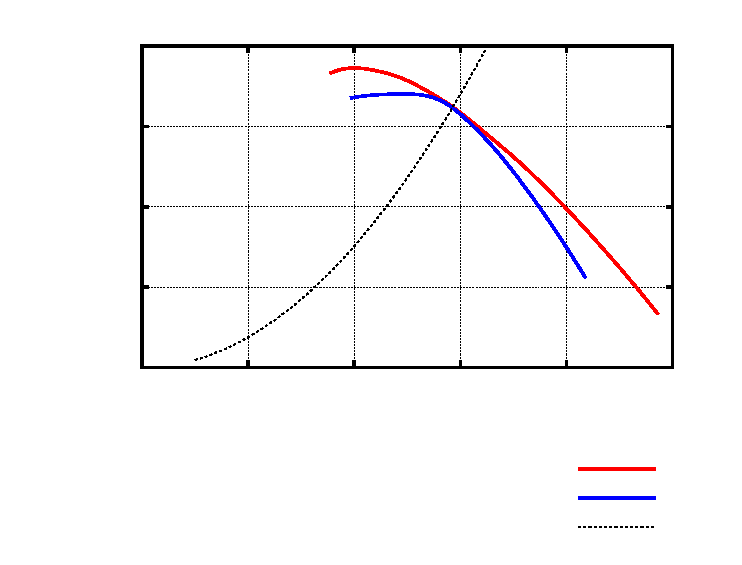
\includegraphics[width={340.10bp},height={255.10bp}]{PQ2}}%
    \gplfronttext
  \end{picture}%
\endgroup

	}
	\caption{Размерные характеристики сравниваемых вентиляторов}
	\label{fig:pq2}
\end{figure}

Безразмерные характеристики этих вентиляторов и сети показаны на рисунке \cref{fig:pq}. В рабочей точке, где пересекаются характеристика сети и характеристика вентилятора, ступени имеют совпадающие развиваемое давление \( P_\nu \) и производительность \(Q\) и имеют примерно одинаковый КПД, но, так как различаются зависимости \(\bar{H}(\bar{c}_{a})\), отличаются частоты вращения необходимые для развития требуемых \(P_{\nu}\) и \(Q\): \(n_1/n_2 = 1,5\), где \(n_{1,2}\) –-- частоты вращения первого и второго колеса.

\begin{figure}[h]
	\centerfloat{	
		% GNUPLOT: LaTeX picture with Postscript
\begingroup
  \makeatletter
  \providecommand\color[2][]{%
    \GenericError{(gnuplot) \space\space\space\@spaces}{%
      Package color not loaded in conjunction with
      terminal option `colourtext'%
    }{See the gnuplot documentation for explanation.%
    }{Either use 'blacktext' in gnuplot or load the package
      color.sty in LaTeX.}%
    \renewcommand\color[2][]{}%
  }%
  \providecommand\includegraphics[2][]{%
    \GenericError{(gnuplot) \space\space\space\@spaces}{%
      Package graphicx or graphics not loaded%
    }{See the gnuplot documentation for explanation.%
    }{The gnuplot epslatex terminal needs graphicx.sty or graphics.sty.}%
    \renewcommand\includegraphics[2][]{}%
  }%
  \providecommand\rotatebox[2]{#2}%
  \@ifundefined{ifGPcolor}{%
    \newif\ifGPcolor
    \GPcolorfalse
  }{}%
  \@ifundefined{ifGPblacktext}{%
    \newif\ifGPblacktext
    \GPblacktexttrue
  }{}%
  % define a \g@addto@macro without @ in the name:
  \let\gplgaddtomacro\g@addto@macro
  % define empty templates for all commands taking text:
  \gdef\gplbacktext{}%
  \gdef\gplfronttext{}%
  \makeatother
  \ifGPblacktext
    % no textcolor at all
    \def\colorrgb#1{}%
    \def\colorgray#1{}%
  \else
    % gray or color?
    \ifGPcolor
      \def\colorrgb#1{\color[rgb]{#1}}%
      \def\colorgray#1{\color[gray]{#1}}%
      \expandafter\def\csname LTw\endcsname{\color{white}}%
      \expandafter\def\csname LTb\endcsname{\color{black}}%
      \expandafter\def\csname LTa\endcsname{\color{black}}%
      \expandafter\def\csname LT0\endcsname{\color[rgb]{1,0,0}}%
      \expandafter\def\csname LT1\endcsname{\color[rgb]{0,1,0}}%
      \expandafter\def\csname LT2\endcsname{\color[rgb]{0,0,1}}%
      \expandafter\def\csname LT3\endcsname{\color[rgb]{1,0,1}}%
      \expandafter\def\csname LT4\endcsname{\color[rgb]{0,1,1}}%
      \expandafter\def\csname LT5\endcsname{\color[rgb]{1,1,0}}%
      \expandafter\def\csname LT6\endcsname{\color[rgb]{0,0,0}}%
      \expandafter\def\csname LT7\endcsname{\color[rgb]{1,0.3,0}}%
      \expandafter\def\csname LT8\endcsname{\color[rgb]{0.5,0.5,0.5}}%
    \else
      % gray
      \def\colorrgb#1{\color{black}}%
      \def\colorgray#1{\color[gray]{#1}}%
      \expandafter\def\csname LTw\endcsname{\color{white}}%
      \expandafter\def\csname LTb\endcsname{\color{black}}%
      \expandafter\def\csname LTa\endcsname{\color{black}}%
      \expandafter\def\csname LT0\endcsname{\color{black}}%
      \expandafter\def\csname LT1\endcsname{\color{black}}%
      \expandafter\def\csname LT2\endcsname{\color{black}}%
      \expandafter\def\csname LT3\endcsname{\color{black}}%
      \expandafter\def\csname LT4\endcsname{\color{black}}%
      \expandafter\def\csname LT5\endcsname{\color{black}}%
      \expandafter\def\csname LT6\endcsname{\color{black}}%
      \expandafter\def\csname LT7\endcsname{\color{black}}%
      \expandafter\def\csname LT8\endcsname{\color{black}}%
    \fi
  \fi
    \setlength{\unitlength}{0.0500bp}%
    \ifx\gptboxheight\undefined%
      \newlength{\gptboxheight}%
      \newlength{\gptboxwidth}%
      \newsavebox{\gptboxtext}%
    \fi%
    \setlength{\fboxrule}{0.5pt}%
    \setlength{\fboxsep}{1pt}%
    \definecolor{tbcol}{rgb}{1,1,1}%
\begin{picture}(6802.00,5102.00)%
    \gplgaddtomacro\gplbacktext{%
      \csname LTb\endcsname%%
      \put(1204,1736){\makebox(0,0)[r]{\strut{}$0$}}%
      \csname LTb\endcsname%%
      \put(1204,2764){\makebox(0,0)[r]{\strut{}$0,05$}}%
      \csname LTb\endcsname%%
      \put(1204,3793){\makebox(0,0)[r]{\strut{}$0,1$}}%
      \csname LTb\endcsname%%
      \put(1204,4821){\makebox(0,0)[r]{\strut{}$0,15$}}%
      \csname LTb\endcsname%%
      \put(1372,1456){\makebox(0,0){\strut{}$0$}}%
      \csname LTb\endcsname%%
      \put(2193,1456){\makebox(0,0){\strut{}$0,1$}}%
      \csname LTb\endcsname%%
      \put(3014,1456){\makebox(0,0){\strut{}$0,2$}}%
      \csname LTb\endcsname%%
      \put(3835,1456){\makebox(0,0){\strut{}$0,3$}}%
      \csname LTb\endcsname%%
      \put(4655,1456){\makebox(0,0){\strut{}$0,4$}}%
      \csname LTb\endcsname%%
      \put(5476,1456){\makebox(0,0){\strut{}$0,5$}}%
      \csname LTb\endcsname%%
      \put(6297,1456){\makebox(0,0){\strut{}$0,6$}}%
    }%
    \gplgaddtomacro\gplfronttext{%
      \csname LTb\endcsname%%
      \put(266,3278){\rotatebox{-270}{\makebox(0,0){\strut{}$\bar{H}$}}}%
      \put(3834,1036){\makebox(0,0){\strut{}$\bar{c}_a$}}%
      \csname LTb\endcsname%%
      \put(5226,763){\makebox(0,0)[r]{\strut{}вентилятор 1}}%
      \csname LTb\endcsname%%
      \put(5226,483){\makebox(0,0)[r]{\strut{}вентилятор 2}}%
      \csname LTb\endcsname%%
      \put(5226,203){\makebox(0,0)[r]{\strut{}сопротивление сети}}%
    }%
    \gplbacktext
    \put(0,0){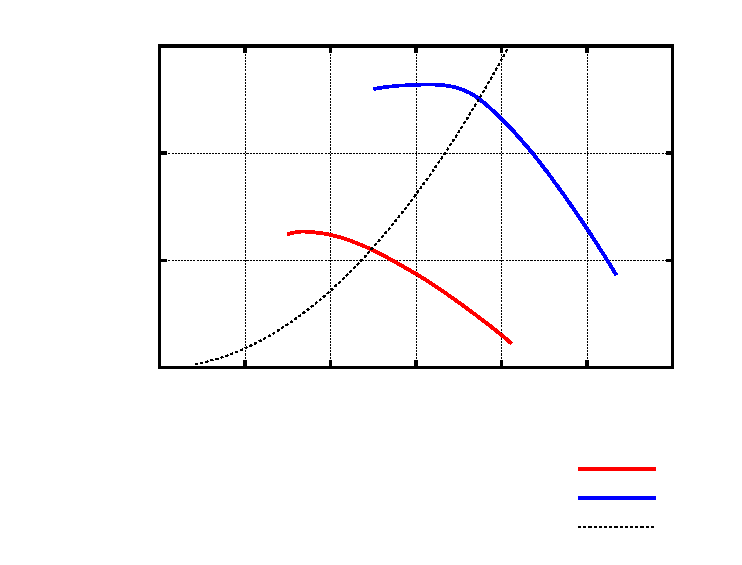
\includegraphics[width={340.10bp},height={255.10bp}]{PQ}}%
    \gplfronttext
  \end{picture}%
\endgroup

	}
	\caption{Безразмерные характеристики сравниваемых вентиляторов}
	\label{fig:pq}
\end{figure}

Механические нагрузки от действующих на лопатку центробежных сил зависят от квадрата частоты вращения рабочего колеса \(n\). При допущении, что лопатки рабочего колеса приблизительно одинаковы у первого и второго вентилятора, напряжения от сил растяжения в корневой части лопатки для второго вентилятора в \((n_1 / n_2)^2  = 2,25\) раз меньше, чем у первого. Однако при одинаковой потребляемой мощности момент на валу привода вентилятора возрастает пропорционально отношению частот вращения \(n_1 / n_2\), соответственно возрастают и механические нагрузки от аэродинамических сил.

Различающиеся частоты вращения приводят к изменениям и акустических характеристик. Разность между уровнями звуковой мощности вентиляторов можно оценить по формуле предложенной Е.Я. Юдиным \cite{Judin1964}:
\begin{equation}
	\Delta L_w=10\log\left[ \frac{\lambda_1(1-\eta_1)}{\lambda_2(1-\eta_2)}\left(\frac{U_\text{к1}}{U_\text{к2}}\right)^6\left(\frac{D_1}{D_2}\right)^2 \right],
	\label{eq:dLw}
\end{equation}
\begin{eqexpl}
	\item{\(\lambda\)} коэффициенты мощности вентиляторов: \(\lambda = 2\Ht\ca (1-\bar{d}^2)\);
	\item{\(\bar{d}\)} относительный диаметр втулки \(d\): \(\bar{d} = d / D\);
	\item{\(\eta\)} коэффициент полезного действия;
	\item{\(U_\text{к}\)} окружная скорость, м/с;
	\item{\(D\)} диаметр рабочего колеса, м.
	\end{eqexpl}

Для двух представленных вентиляторов с разной частотой  вращения разница мощности акустического излучения \( \Delta L_w \) по формуле \ref{eq:dLw} составляет приблизительно 5,3 дБ. 


\section{Ограничения на величину коэффициента теоретического напора}\label{ch1/sec3}

Типичные значения коэффициента теоретического напора \(\Ht\) осевого вентилятора или ступени компрессора находятся в пределах от 0,2 до 0,4 и редко превышают 0,45 при коэффициенте расхода \(\ca\) в диапазоне от 0,4 до 0,6. Влияние выбранных параметров \(\Ht\) и \(\ca\) на КПД $\eta$ компрессора иллюстрируется рисунком \cref{fig:etaFromHtCa} из работы \cite{Hall2012}. В границах типичных значений \(\Ht\) и \(\ca\) значение $\eta$ не сильно отличается от максимального и выход за типичные пределы значений, особенно в область высоких \(\Ht\), ведёт к резкому снижению КПД. Необходимые большие углы поворота потока требуют увеличения густоты решёток профилей и росту профильных потерь \cite{Howell1945, Bunimovich1967}. 
\begin{figure}[ht]
	\centerfloat{
		\begin{tabular}{m{0.5cm}m{240pt}}
			\multicolumn{1}{r}{\rotatebox{90}{$\Ht$}} & 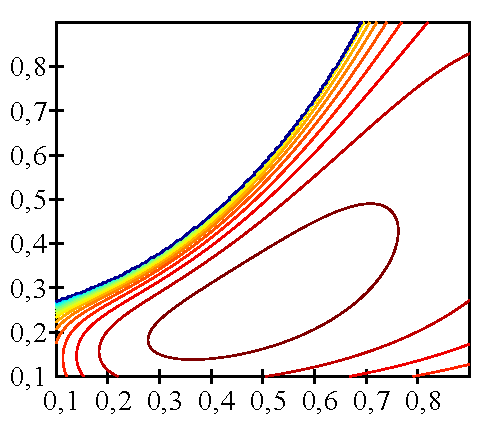
\includegraphics{images/11zon_cropped.pdf} \\
			& \multicolumn{1}{c}{$\ca$}\\
		\end{tabular}
	}
	\caption{Зависимость $\eta$ от сочетания параметров \(\Ht\) и \(\ca\) \cite{Hall2012}. Шаг между изолиниями 1\%; максимум 95\%}
	\label{fig:etaFromHtCa}
\end{figure}

В работе \cite{Dickens2011} исследовалась возможность применения высокого значения \(\Ht\) и его влияние на КПД ступени. При повышении \(\Ht\) с 0,45 до 0,55 адиабатический КПД ступени снизился примерно на 0,9\% и составил 86\%, а при повышении от 0,55 до 0,65 снизился ещё на 2,5\%. Коэффициент расхода \(\ca\) во всех случаях составлял 0,5. Рост потерь давления был связан с повышением толщины потери импульса $\delta_{2}$  на поверхностях лопатки. КПД спрямляющего аппарата оказался более чувствителен к изменению \(\Ht\), чем КПД рабочего колеса. Эффективное повышение \(\Ht\) потребовало увеличить степень реактивности ступени, то есть отношение работы сжатия в РК к работе сжатия во всей ступени.

Влияние выбора расчётных параметров \(\Ht\) и \(\ca\) на КПД вентилятора \(\eta\) для схемы состоящей из рабочего колеса и спрямляющего аппарата (РК+СА) можно оценить по графику \cref{fig:BrusEtaFromHtCa} из работы \cite{Brusilovskiy1986}. C ростом \(\Ht\) уменьшается $\eta$. Максимум $\eta$ так же снижается и смещается в сторону меньших \(\ca\), так как при б\'ольших \(\ca\) уменьшается \(\eta\) СА.
\begin{figure}[ht]
	\centerfloat{
		% GNUPLOT: LaTeX picture with Postscript
\begingroup
  \makeatletter
  \providecommand\color[2][]{%
    \GenericError{(gnuplot) \space\space\space\@spaces}{%
      Package color not loaded in conjunction with
      terminal option `colourtext'%
    }{See the gnuplot documentation for explanation.%
    }{Either use 'blacktext' in gnuplot or load the package
      color.sty in LaTeX.}%
    \renewcommand\color[2][]{}%
  }%
  \providecommand\includegraphics[2][]{%
    \GenericError{(gnuplot) \space\space\space\@spaces}{%
      Package graphicx or graphics not loaded%
    }{See the gnuplot documentation for explanation.%
    }{The gnuplot epslatex terminal needs graphicx.sty or graphics.sty.}%
    \renewcommand\includegraphics[2][]{}%
  }%
  \providecommand\rotatebox[2]{#2}%
  \@ifundefined{ifGPcolor}{%
    \newif\ifGPcolor
    \GPcolorfalse
  }{}%
  \@ifundefined{ifGPblacktext}{%
    \newif\ifGPblacktext
    \GPblacktexttrue
  }{}%
  % define a \g@addto@macro without @ in the name:
  \let\gplgaddtomacro\g@addto@macro
  % define empty templates for all commands taking text:
  \gdef\gplbacktext{}%
  \gdef\gplfronttext{}%
  \makeatother
  \ifGPblacktext
    % no textcolor at all
    \def\colorrgb#1{}%
    \def\colorgray#1{}%
  \else
    % gray or color?
    \ifGPcolor
      \def\colorrgb#1{\color[rgb]{#1}}%
      \def\colorgray#1{\color[gray]{#1}}%
      \expandafter\def\csname LTw\endcsname{\color{white}}%
      \expandafter\def\csname LTb\endcsname{\color{black}}%
      \expandafter\def\csname LTa\endcsname{\color{black}}%
      \expandafter\def\csname LT0\endcsname{\color[rgb]{1,0,0}}%
      \expandafter\def\csname LT1\endcsname{\color[rgb]{0,1,0}}%
      \expandafter\def\csname LT2\endcsname{\color[rgb]{0,0,1}}%
      \expandafter\def\csname LT3\endcsname{\color[rgb]{1,0,1}}%
      \expandafter\def\csname LT4\endcsname{\color[rgb]{0,1,1}}%
      \expandafter\def\csname LT5\endcsname{\color[rgb]{1,1,0}}%
      \expandafter\def\csname LT6\endcsname{\color[rgb]{0,0,0}}%
      \expandafter\def\csname LT7\endcsname{\color[rgb]{1,0.3,0}}%
      \expandafter\def\csname LT8\endcsname{\color[rgb]{0.5,0.5,0.5}}%
    \else
      % gray
      \def\colorrgb#1{\color{black}}%
      \def\colorgray#1{\color[gray]{#1}}%
      \expandafter\def\csname LTw\endcsname{\color{white}}%
      \expandafter\def\csname LTb\endcsname{\color{black}}%
      \expandafter\def\csname LTa\endcsname{\color{black}}%
      \expandafter\def\csname LT0\endcsname{\color{black}}%
      \expandafter\def\csname LT1\endcsname{\color{black}}%
      \expandafter\def\csname LT2\endcsname{\color{black}}%
      \expandafter\def\csname LT3\endcsname{\color{black}}%
      \expandafter\def\csname LT4\endcsname{\color{black}}%
      \expandafter\def\csname LT5\endcsname{\color{black}}%
      \expandafter\def\csname LT6\endcsname{\color{black}}%
      \expandafter\def\csname LT7\endcsname{\color{black}}%
      \expandafter\def\csname LT8\endcsname{\color{black}}%
    \fi
  \fi
    \setlength{\unitlength}{0.0500bp}%
    \ifx\gptboxheight\undefined%
      \newlength{\gptboxheight}%
      \newlength{\gptboxwidth}%
      \newsavebox{\gptboxtext}%
    \fi%
    \setlength{\fboxrule}{0.5pt}%
    \setlength{\fboxsep}{1pt}%
    \definecolor{tbcol}{rgb}{1,1,1}%
\begin{picture}(6802.00,5102.00)%
    \gplgaddtomacro\gplbacktext{%
      \csname LTb\endcsname%%
      \put(1204,1456){\makebox(0,0)[r]{\strut{}$0,8$}}%
      \csname LTb\endcsname%%
      \put(1204,2129){\makebox(0,0)[r]{\strut{}$0,82$}}%
      \csname LTb\endcsname%%
      \put(1204,2802){\makebox(0,0)[r]{\strut{}$0,84$}}%
      \csname LTb\endcsname%%
      \put(1204,3475){\makebox(0,0)[r]{\strut{}$0,86$}}%
      \csname LTb\endcsname%%
      \put(1204,4148){\makebox(0,0)[r]{\strut{}$0,88$}}%
      \csname LTb\endcsname%%
      \put(1204,4821){\makebox(0,0)[r]{\strut{}$0,9$}}%
      \csname LTb\endcsname%%
      \put(1372,1176){\makebox(0,0){\strut{}$0,4$}}%
      \csname LTb\endcsname%%
      \put(2193,1176){\makebox(0,0){\strut{}$0,5$}}%
      \csname LTb\endcsname%%
      \put(3014,1176){\makebox(0,0){\strut{}$0,6$}}%
      \csname LTb\endcsname%%
      \put(3834,1176){\makebox(0,0){\strut{}$0,7$}}%
      \csname LTb\endcsname%%
      \put(4655,1176){\makebox(0,0){\strut{}$0,8$}}%
      \csname LTb\endcsname%%
      \put(5476,1176){\makebox(0,0){\strut{}$0,9$}}%
      \csname LTb\endcsname%%
      \put(6297,1176){\makebox(0,0){\strut{}$1$}}%
    }%
    \gplgaddtomacro\gplfronttext{%
      \csname LTb\endcsname%%
      \put(266,3138){\rotatebox{-270}{\makebox(0,0){\strut{}$\eta$}}}%
      \put(3834,756){\makebox(0,0){\strut{}$\bar{c}_a$}}%
      \put(1500,320){\makebox(0,0){\strut{}$\bar{H}_\text{т}:$}}%
      \csname LTb\endcsname%%
      \put(2763,483){\makebox(0,0)[r]{\strut{}0,05}}%
      \csname LTb\endcsname%%
      \put(2763,203){\makebox(0,0)[r]{\strut{}0,1}}%
      \csname LTb\endcsname%%
      \put(4506,483){\makebox(0,0)[r]{\strut{}0,2}}%
      \csname LTb\endcsname%%
      \put(4506,203){\makebox(0,0)[r]{\strut{}0,4}}%
    }%
    \gplbacktext
    \put(0,0){\includegraphics[width={340.10bp},height={255.10bp}]{BrusEta}}%
    \gplfronttext
  \end{picture}%
\endgroup

	}
	\caption{Зависимость $\eta$ схемы РК+СА от расчётных значений \(\Ht\)~и~\(\ca\)}
	\label{fig:BrusEtaFromHtCa}
\end{figure}
\section{Пределы аэродинамической нагруженности}\label{ch1/sec4}

Для течения в лопаточных венцах вентилятора характерно существование таких режимов работы, при которых происходит образование отрывных зон приводящих к резкому снижению КПД. Близость режима возникновения отрыва потока в проточной части вентилятора к его расчетному режиму характеризуется аэродинамической нагруженностью лопаточных венцов. Для различных элементов проточной части отличаются факторы возникновения и механизмы развития отрыва. Для оценки аэродинамической нагруженности по каждому из факторов разработаны отдельные критерии.

\subsection{Вязкий отрыв пограничного слоя}\label{ch1/sec5}

Отрыв потока от поверхностей лопатки и элементов проточной части вентилятора обусловленный вязкостью воздуха происходит в связи с наличием пограничного слоя. На жидкие частицы в пограничном слое действуют значительные касательные напряжения, при приближении к поверхности происходит резкое снижение скорости и кинетической энергии. При диффузорном течении статическое давление увеличивается по ходу движения газа, и пристеночные слои воздуха подтормаживаются сильнее, пока им достаточно энергии для преодоления градиента давления, после чего останавливаются. В точке остановки слоя воздуха происходит отрыв пограничного слоя от поверхности, ниже по течению появляются области обратного течения, основной поток отходит от поверхности и ускоряется, что приводит к росту потерь полного давления. 

Для оценки аэродинамической нагруженности с точки зрения вязкого отрыва пограничного слоя потока в решетках профилей разными авторами был предложен ряд критериев. К примеру, величина произведения густоты решётки на коэффициент подъёмной силы профиля $\tau C_y$ \cite{Hausenblas1963,Dovjik1968} и угол раскрытия эквивалентного диффузора \(\gamma\) \cite{Dovjik1958,Uschakov1963}. Большое распространение получил фактор эквивалентной диффузорности Либляйна \cite{Lieblein1959}:
\begin{equation}
	D_\text{eq} = \frac{\cos \beta_2}{\cos \beta_1} \left[ 1,12 + 0,61\frac{\cos^2\beta_1}{\tau}(\tan \beta_1 - \tan\beta_2) \right],
	\label{eq:DeqLieblein}
\end{equation}
\begin{eqexpl}
	\item{$\beta_{1,2}$} угол между скоростью потока в относительном движении перед (1) и за (2) решёткой профилей и осью решетки;
	\item{$\tau$} густота решетки.
\end{eqexpl}

Этот фактор разработан для плоских решёток составленных из профилей NACA"--~65 работающих на режиме минимальных потерь, но применяется для широкого класса задач. Либляйн применил его при анализе материалов экспериментальных продувок решёток профилей с углом атаки превышающем угол соответствующий режиму работы решётки с минимальным уровнем потерь (рисунок \ref{fig:DeqLieblein}). Был установлен резкий рост толщины потери импульса $\delta_2$ и отрыв потока при превышении величины $D_\text{eq}$ значения приблизительно равного 2 \cite{Lieblein1959}. При предварительном профилировании лопаток осевого вентилятора, благодаря простоте выражения \ref{eq:DeqLieblein}, удобно использовать $D_\text{eq}$ при анализе вариантов геометрии.
\begin{figure}[ht]
\centerfloat{
\begin{tabular}{m{0.5cm}m{12cm}}
\multicolumn{1}{r}{\rotatebox{90}{$\delta_2/c$}} & 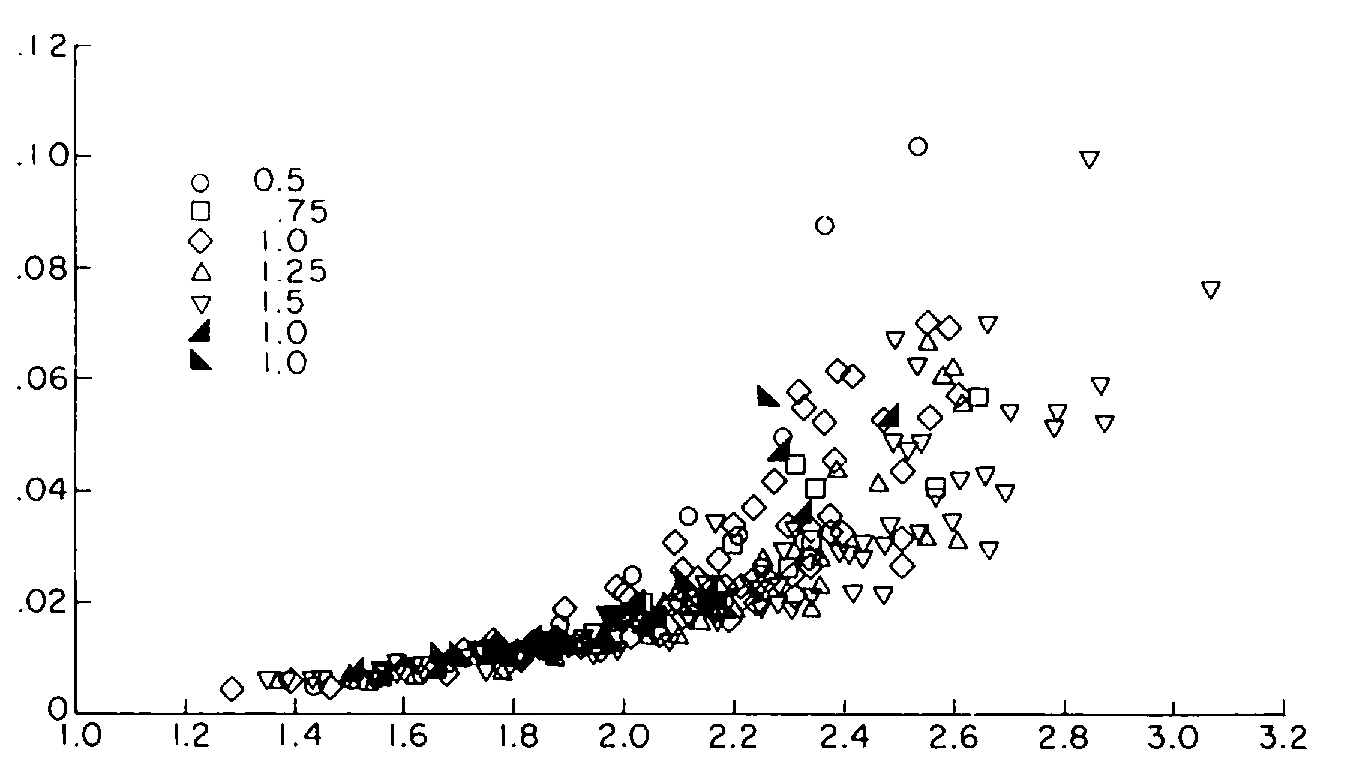
\includegraphics{images/DeqLeiblein.png} \\
   & \multicolumn{1}{c}{$D_\text{eq}$}\\
\end{tabular}	
}
	\caption{Рост толщины потери импульса отнесённой к хорде профиля~$\delta_2/c$ в зависимости от $D_\text{eq}$ \cite{Lieblein1959}}
	\label{fig:DeqLieblein}
\end{figure}

Течение в лопаточных венцах вентиляторов отличается от течения в плоских решётках, которое часто рассматривается при упрощении. Особенно значительные отличия проявляются в концевых областях, где взаимодействуют пограничные слои на лопатках и торцевых поверхностях вызывая вторичные течения. 
Во вращающихся венцах характер вторичных течений изменяется под действием центробежных сил на пограничный слой. Заторможенные в пограничном слое лопатки жидкие частицы перемещаются к периферии. В привтулочных сечениях лопатки влияние пограничного слоя ослабляется, а в периферийных, наоборот, усиливается. Соответственно меняется и аэродинамическая нагруженность в сравнении с нагруженностью плоской решётки \cite{Brusilovskiy1986}. Это позволяет выбирать несколько меньшую густоту решётки у втулки и большую у периферии, чем это следует из обобщённых продувок плоских решёток профилей.

\subsection{Потеря устойчивости вращающегося потока}\label{ch1/sec6}

В закрученных потоках давление уменьшается в направлении от периферии к оси вращения. На жидкие частицы в разных направлениях действуют силы инерции и силы давления, что обеспечивает радиальное равновесие \cite{Smith1966}. При достаточной интенсивности закрутки равновесие нарушается, в приосевой части течения возможно образование замкнутых циркуляционных зон. При проектировании ряда устройств, к примеру вихревых горелках или циклонных сепараторах, образование таких зон заложено намерено для стабилизации пламени, обеспечения полноты сгорания или разделения фракций разной плотности \cite{Gupta1987, Goldschtik1981}.
Ключевым критерием подобия в закрученных течениях является параметр закрутки \(S\):
\begin{equation}
	S = \frac{G_\theta}{G_x R},
	\label{eq:S}
\end{equation}
\begin{eqexpl}
	\item{\(G_\theta\)} поток момента количества движения, \(\si\kilogram\cdot\si\meter^2/\si\second^2\);
	\item{\(G_x\)} поток количества движения, \(\si\kilogram\cdot\si\meter/\si\second^2\);
	\item{\(R\)} радиус сопла, \(\si\meter\).
\end{eqexpl}

В турбомашинах так же могут возникать циркуляционные зоны, например, в последних ступенях паровых турбин \cite{Bammert1949} или в осевых вентиляторах с большой долей статического давления в полном \cite{Mitrofovich1991}. Незапланированные зоны отрыва ведут к изменению структуры потока и нарушению нормальной работы машины. Циркуляционные зоны (рисунок \ref{fig:Mitrof1999}) при таком типе отрыва начинают развитие у выходной кромки втулки и распространяются вверх по потоку, увеличивая свои размеры и интенсивность, являясь при этом нестационарными и вращающимися в направлении закрутки потока \cite{Mitrofovich1999}. 
\begin{figure} [ht]
	\centerfloat{
		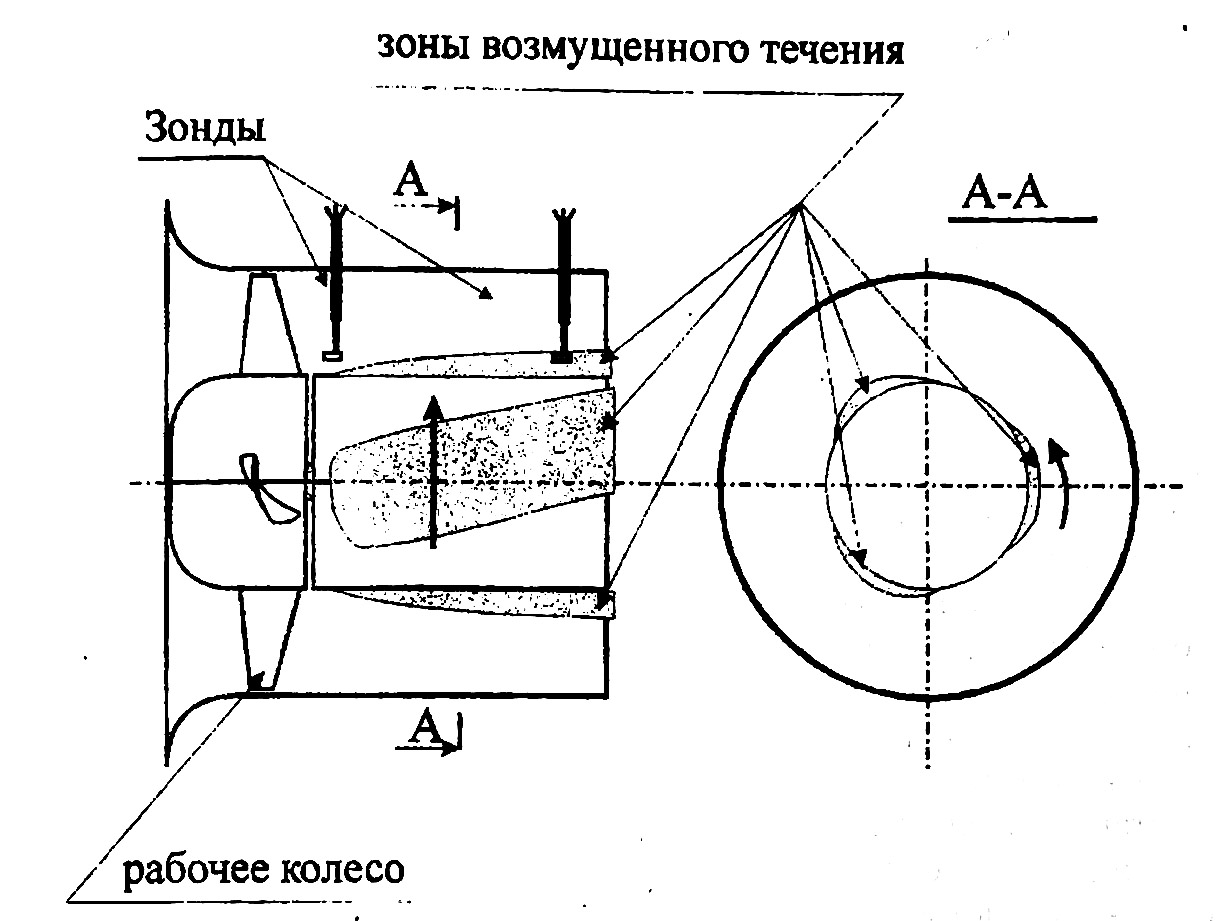
\includegraphics[width=12cm,keepaspectratio]{images/Mitrof1999}
	}
		\caption{Схема отрывных зон при потери устойчивости течения у втулки за осевым вентилятором \cite{Mitrofovich1999}}
	\label{fig:Mitrof1999}
\end{figure}

Для вентилятора состоящему только из рабочего колеса спрофилированного по закону постоянной циркуляции (\(C_u r = \text{const}\)), используется обратный критерий записанный через безразмерные параметры \(\bar{d}\ca/\Ht\). Опираясь на это число, можно определить радиус циркуляционной зоны, возникающей при распаде вихря при течении в трубе \cite{Strscheletzky1955}. В зависимости от кинематики потока и геометрии проточной части вентилятора циркуляционные зоны возникают вместе с отрывом потока от поверхности втулки \cite{Mitrofovich1991}, граница допустимых сочетаний параметров показана на графике \ref{fig:RoMitrof}. 
\begin{figure} [ht]
	\centerfloat{
	 % GNUPLOT: LaTeX picture with Postscript
\begingroup
  \makeatletter
  \providecommand\color[2][]{%
    \GenericError{(gnuplot) \space\space\space\@spaces}{%
      Package color not loaded in conjunction with
      terminal option `colourtext'%
    }{See the gnuplot documentation for explanation.%
    }{Either use 'blacktext' in gnuplot or load the package
      color.sty in LaTeX.}%
    \renewcommand\color[2][]{}%
  }%
  \providecommand\includegraphics[2][]{%
    \GenericError{(gnuplot) \space\space\space\@spaces}{%
      Package graphicx or graphics not loaded%
    }{See the gnuplot documentation for explanation.%
    }{The gnuplot epslatex terminal needs graphicx.sty or graphics.sty.}%
    \renewcommand\includegraphics[2][]{}%
  }%
  \providecommand\rotatebox[2]{#2}%
  \@ifundefined{ifGPcolor}{%
    \newif\ifGPcolor
    \GPcolorfalse
  }{}%
  \@ifundefined{ifGPblacktext}{%
    \newif\ifGPblacktext
    \GPblacktexttrue
  }{}%
  % define a \g@addto@macro without @ in the name:
  \let\gplgaddtomacro\g@addto@macro
  % define empty templates for all commands taking text:
  \gdef\gplbacktext{}%
  \gdef\gplfronttext{}%
  \makeatother
  \ifGPblacktext
    % no textcolor at all
    \def\colorrgb#1{}%
    \def\colorgray#1{}%
  \else
    % gray or color?
    \ifGPcolor
      \def\colorrgb#1{\color[rgb]{#1}}%
      \def\colorgray#1{\color[gray]{#1}}%
      \expandafter\def\csname LTw\endcsname{\color{white}}%
      \expandafter\def\csname LTb\endcsname{\color{black}}%
      \expandafter\def\csname LTa\endcsname{\color{black}}%
      \expandafter\def\csname LT0\endcsname{\color[rgb]{1,0,0}}%
      \expandafter\def\csname LT1\endcsname{\color[rgb]{0,1,0}}%
      \expandafter\def\csname LT2\endcsname{\color[rgb]{0,0,1}}%
      \expandafter\def\csname LT3\endcsname{\color[rgb]{1,0,1}}%
      \expandafter\def\csname LT4\endcsname{\color[rgb]{0,1,1}}%
      \expandafter\def\csname LT5\endcsname{\color[rgb]{1,1,0}}%
      \expandafter\def\csname LT6\endcsname{\color[rgb]{0,0,0}}%
      \expandafter\def\csname LT7\endcsname{\color[rgb]{1,0.3,0}}%
      \expandafter\def\csname LT8\endcsname{\color[rgb]{0.5,0.5,0.5}}%
    \else
      % gray
      \def\colorrgb#1{\color{black}}%
      \def\colorgray#1{\color[gray]{#1}}%
      \expandafter\def\csname LTw\endcsname{\color{white}}%
      \expandafter\def\csname LTb\endcsname{\color{black}}%
      \expandafter\def\csname LTa\endcsname{\color{black}}%
      \expandafter\def\csname LT0\endcsname{\color{black}}%
      \expandafter\def\csname LT1\endcsname{\color{black}}%
      \expandafter\def\csname LT2\endcsname{\color{black}}%
      \expandafter\def\csname LT3\endcsname{\color{black}}%
      \expandafter\def\csname LT4\endcsname{\color{black}}%
      \expandafter\def\csname LT5\endcsname{\color{black}}%
      \expandafter\def\csname LT6\endcsname{\color{black}}%
      \expandafter\def\csname LT7\endcsname{\color{black}}%
      \expandafter\def\csname LT8\endcsname{\color{black}}%
    \fi
  \fi
    \setlength{\unitlength}{0.0500bp}%
    \ifx\gptboxheight\undefined%
      \newlength{\gptboxheight}%
      \newlength{\gptboxwidth}%
      \newsavebox{\gptboxtext}%
    \fi%
    \setlength{\fboxrule}{0.5pt}%
    \setlength{\fboxsep}{1pt}%
    \definecolor{tbcol}{rgb}{1,1,1}%
\begin{picture}(6802.00,5102.00)%
    \gplgaddtomacro\gplbacktext{%
      \csname LTb\endcsname%%
      \put(1036,896){\makebox(0,0)[r]{\strut{}$0,4$}}%
      \csname LTb\endcsname%%
      \put(1036,1877){\makebox(0,0)[r]{\strut{}$0,6$}}%
      \csname LTb\endcsname%%
      \put(1036,2859){\makebox(0,0)[r]{\strut{}$0,8$}}%
      \csname LTb\endcsname%%
      \put(1036,3840){\makebox(0,0)[r]{\strut{}$1$}}%
      \csname LTb\endcsname%%
      \put(1036,4821){\makebox(0,0)[r]{\strut{}$1,2$}}%
      \csname LTb\endcsname%%
      \put(1204,616){\makebox(0,0){\strut{}$1$}}%
      \csname LTb\endcsname%%
      \put(2053,616){\makebox(0,0){\strut{}$1,5$}}%
      \csname LTb\endcsname%%
      \put(2902,616){\makebox(0,0){\strut{}$2$}}%
      \csname LTb\endcsname%%
      \put(3751,616){\makebox(0,0){\strut{}$2,5$}}%
      \csname LTb\endcsname%%
      \put(4599,616){\makebox(0,0){\strut{}$3$}}%
      \csname LTb\endcsname%%
      \put(5448,616){\makebox(0,0){\strut{}$3,5$}}%
      \csname LTb\endcsname%%
      \put(6297,616){\makebox(0,0){\strut{}$4$}}%
    }%
    \gplgaddtomacro\gplfronttext{%
      \csname LTb\endcsname%%
      \put(266,2858){\rotatebox{-270}{\makebox(0,0){\strut{}$\bar{d}\ca/\Ht$}}}%
      \put(3750,196){\makebox(0,0){\strut{}$\tan \beta_1$}}%
    }%
    \gplbacktext
    \put(0,0){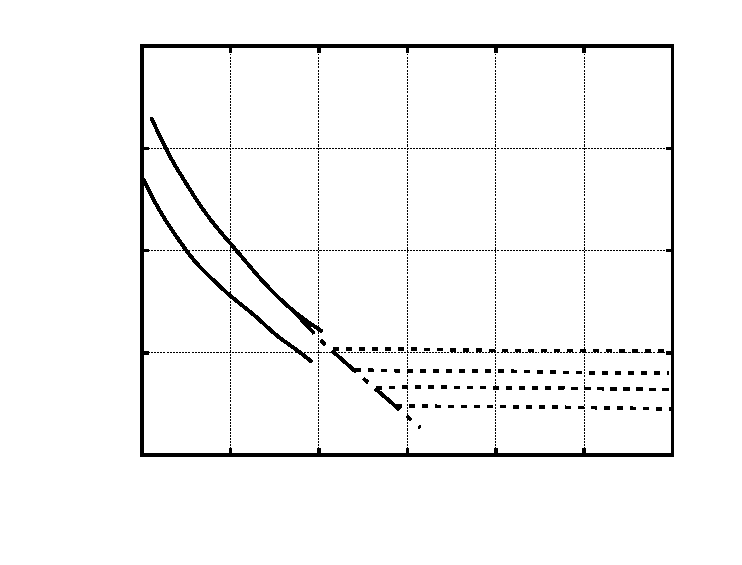
\includegraphics[width={340.10bp},height={255.10bp}]{Mitrof1991}}%
    \gplfronttext
  \end{picture}%
\endgroup

	 
	 \begin{eqexpl}
	 	\item{\(\beta_1\)} угол между направлением скорости потока перед решёткой и осью решётки;
	 \end{eqexpl}
	}
	\caption{Границы существования высокоэффективных вентиляторов различных аэродинамических схем \cite{Mitrofovich1991}}
	\label{fig:RoMitrof}
\end{figure}

\subsection{Методы снижения аэродинамической нагруженности}\label{ch1/sec7}

С целью повышения эффективности или расширения диапазона рабочих режимов для улучшения аэродинамических или эксплуатационных характеристик машин и аппаратов производится управление пограничным слоем. Управление производится в виде уменьшения влияния пограничного слоя на течение, путём либо изменения формы тела так, чтобы сохранить высокий уровень энергии вблизи поверхности, либо повышения уровня энергии с помощью дополнительных устройств. Широкий обзор методов управления отрывом потока дан в монографии  \cite{Chen1979}.

В высоконагруженных ступенях осевых вентиляторов наличие небольших локальных отрывных пузырей на поверхности лопатки у втулки и у задней кромки не оказывает значительного негативного влияния на аэродинамические характеристики. С точки зрения эффективности выгоднее лишь ослабить влияние отрывных зон чем полностью их ликвидировать \cite{Chen1979}.

Течение в диффузорных решётках сопряжено с градиентом давления на спинке профилей и возможностью отрыва потока. Управление пограничным слоем с помощью специального профилирования \cite{Papailiou1970,Hobbs1984,Meng2023}, обеспечивающего предварительно заданное распределение давления на спинке профиля, позволяет снижать профильные потери полного давления. Контроль над местом ламинарно-турбулентного перехода и состоянием пограничного слоя снижает аэродинамическую нагруженность решётки и позволяет выбирать меньшие густоты, чем при использовании обычных серий профилей. Однако такие профили требуют повышенной точности исполнения.

Главное преимущество такого подхода к профилированию заключается в том, чтобы снизить максимальные местные числа Маха на спинке профиля для предотвращения возникновения локальных скачков уплотнения, повышающих потери давления и провоцирующих отрыв пограничного слоя. В работе \cite{Hobbs1984} для одного режима работы двух решёток профилей приведено сравнение коэффициента потерь полного давления \(\zeta = \Delta P /0,5 \rho W_1^2\), (где \(\Delta P\) "--- потери полного давления, Па; \(W_1\) "--- скорость перед решёткой, \(\si\meter/\si\second\)) в зависимости от числа Маха на входе в решётку \(M_1\) (рисунок \ref{fig:Hobbs1984}). Профили первой решётки были специально спрофилированы, вторые выбраны из серии профилей NACA-400. Специальное профилирование позволило получить меньшие потери при умеренных числах \(M_1\) до 0,7, и большее критическое число Маха, при котором потери начинают резко расти. 
\begin{figure} [ht]
	\centerfloat{
		% GNUPLOT: LaTeX picture with Postscript
\begingroup
  \makeatletter
  \providecommand\color[2][]{%
    \GenericError{(gnuplot) \space\space\space\@spaces}{%
      Package color not loaded in conjunction with
      terminal option `colourtext'%
    }{See the gnuplot documentation for explanation.%
    }{Either use 'blacktext' in gnuplot or load the package
      color.sty in LaTeX.}%
    \renewcommand\color[2][]{}%
  }%
  \providecommand\includegraphics[2][]{%
    \GenericError{(gnuplot) \space\space\space\@spaces}{%
      Package graphicx or graphics not loaded%
    }{See the gnuplot documentation for explanation.%
    }{The gnuplot epslatex terminal needs graphicx.sty or graphics.sty.}%
    \renewcommand\includegraphics[2][]{}%
  }%
  \providecommand\rotatebox[2]{#2}%
  \@ifundefined{ifGPcolor}{%
    \newif\ifGPcolor
    \GPcolorfalse
  }{}%
  \@ifundefined{ifGPblacktext}{%
    \newif\ifGPblacktext
    \GPblacktexttrue
  }{}%
  % define a \g@addto@macro without @ in the name:
  \let\gplgaddtomacro\g@addto@macro
  % define empty templates for all commands taking text:
  \gdef\gplbacktext{}%
  \gdef\gplfronttext{}%
  \makeatother
  \ifGPblacktext
    % no textcolor at all
    \def\colorrgb#1{}%
    \def\colorgray#1{}%
  \else
    % gray or color?
    \ifGPcolor
      \def\colorrgb#1{\color[rgb]{#1}}%
      \def\colorgray#1{\color[gray]{#1}}%
      \expandafter\def\csname LTw\endcsname{\color{white}}%
      \expandafter\def\csname LTb\endcsname{\color{black}}%
      \expandafter\def\csname LTa\endcsname{\color{black}}%
      \expandafter\def\csname LT0\endcsname{\color[rgb]{1,0,0}}%
      \expandafter\def\csname LT1\endcsname{\color[rgb]{0,1,0}}%
      \expandafter\def\csname LT2\endcsname{\color[rgb]{0,0,1}}%
      \expandafter\def\csname LT3\endcsname{\color[rgb]{1,0,1}}%
      \expandafter\def\csname LT4\endcsname{\color[rgb]{0,1,1}}%
      \expandafter\def\csname LT5\endcsname{\color[rgb]{1,1,0}}%
      \expandafter\def\csname LT6\endcsname{\color[rgb]{0,0,0}}%
      \expandafter\def\csname LT7\endcsname{\color[rgb]{1,0.3,0}}%
      \expandafter\def\csname LT8\endcsname{\color[rgb]{0.5,0.5,0.5}}%
    \else
      % gray
      \def\colorrgb#1{\color{black}}%
      \def\colorgray#1{\color[gray]{#1}}%
      \expandafter\def\csname LTw\endcsname{\color{white}}%
      \expandafter\def\csname LTb\endcsname{\color{black}}%
      \expandafter\def\csname LTa\endcsname{\color{black}}%
      \expandafter\def\csname LT0\endcsname{\color{black}}%
      \expandafter\def\csname LT1\endcsname{\color{black}}%
      \expandafter\def\csname LT2\endcsname{\color{black}}%
      \expandafter\def\csname LT3\endcsname{\color{black}}%
      \expandafter\def\csname LT4\endcsname{\color{black}}%
      \expandafter\def\csname LT5\endcsname{\color{black}}%
      \expandafter\def\csname LT6\endcsname{\color{black}}%
      \expandafter\def\csname LT7\endcsname{\color{black}}%
      \expandafter\def\csname LT8\endcsname{\color{black}}%
    \fi
  \fi
    \setlength{\unitlength}{0.0500bp}%
    \ifx\gptboxheight\undefined%
      \newlength{\gptboxheight}%
      \newlength{\gptboxwidth}%
      \newsavebox{\gptboxtext}%
    \fi%
    \setlength{\fboxrule}{0.5pt}%
    \setlength{\fboxsep}{1pt}%
    \definecolor{tbcol}{rgb}{1,1,1}%
\begin{picture}(6802.00,5102.00)%
    \gplgaddtomacro\gplbacktext{%
      \csname LTb\endcsname%%
      \put(1204,1456){\makebox(0,0)[r]{\strut{}$0,01$}}%
      \csname LTb\endcsname%%
      \put(1204,2017){\makebox(0,0)[r]{\strut{}$0,02$}}%
      \csname LTb\endcsname%%
      \put(1204,2578){\makebox(0,0)[r]{\strut{}$0,03$}}%
      \csname LTb\endcsname%%
      \put(1204,3139){\makebox(0,0)[r]{\strut{}$0,04$}}%
      \csname LTb\endcsname%%
      \put(1204,3699){\makebox(0,0)[r]{\strut{}$0,05$}}%
      \csname LTb\endcsname%%
      \put(1204,4260){\makebox(0,0)[r]{\strut{}$0,06$}}%
      \csname LTb\endcsname%%
      \put(1204,4821){\makebox(0,0)[r]{\strut{}$0,07$}}%
      \csname LTb\endcsname%%
      \put(1372,1176){\makebox(0,0){\strut{}$0,3$}}%
      \csname LTb\endcsname%%
      \put(2193,1176){\makebox(0,0){\strut{}$0,4$}}%
      \csname LTb\endcsname%%
      \put(3014,1176){\makebox(0,0){\strut{}$0,5$}}%
      \csname LTb\endcsname%%
      \put(3834,1176){\makebox(0,0){\strut{}$0,6$}}%
      \csname LTb\endcsname%%
      \put(4655,1176){\makebox(0,0){\strut{}$0,7$}}%
      \csname LTb\endcsname%%
      \put(5476,1176){\makebox(0,0){\strut{}$0,8$}}%
      \csname LTb\endcsname%%
      \put(6297,1176){\makebox(0,0){\strut{}$0,9$}}%
    }%
    \gplgaddtomacro\gplfronttext{%
      \csname LTb\endcsname%%
      \put(266,3138){\rotatebox{-270}{\makebox(0,0){\strut{}$\zeta$}}}%
      \put(3834,756){\makebox(0,0){\strut{}$M_1$}}%
      \csname LTb\endcsname%%
      \put(5226,483){\makebox(0,0)[r]{\strut{}специальное профилирование}}%
      \csname LTb\endcsname%%
      \put(5226,203){\makebox(0,0)[r]{\strut{}профили NACA-405}}%
    }%
    \gplbacktext
    \put(0,0){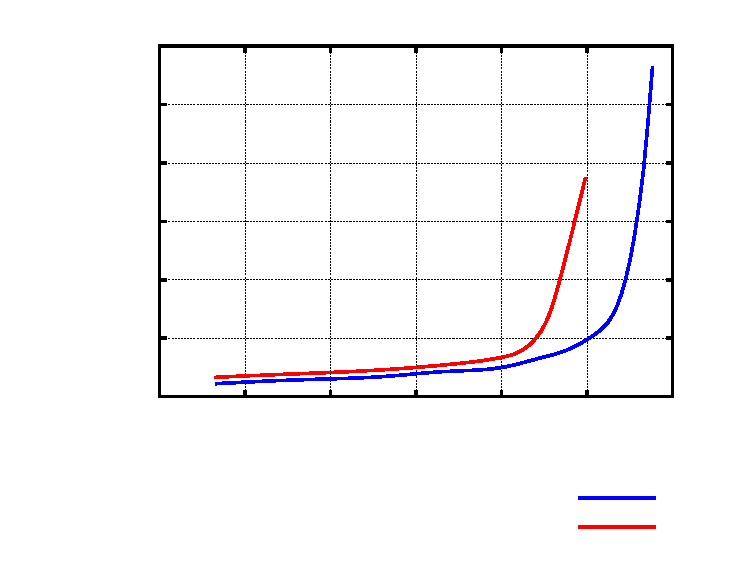
\includegraphics[width={340.10bp},height={255.10bp}]{Hobbs1984}}%
    \gplfronttext
  \end{picture}%
\endgroup

	}
	\caption{Сопоставление коэффициента потерь \(\zeta\) в решётках с профилями с специальным профилированием и серии NACA-400 при разных числах маха на входе \(M_1\) \cite{Hobbs1984}}
	\label{fig:Hobbs1984}
\end{figure}

Широкое исследование методов аэродинамического совершенствования высоконагруженных лопаточных аппаратов компрессоров выполнено в работе \cite{Tereschenko1988}. Рассматриваются активные методы управления пограничным слоем такие как вдув струй в пограничный слой, отсос пограничного слоя и пассивные, такие как применение двухрядных решёток и трубулизаторов  потока (рисунок \ref{fig:Tereshenko1988}).

\begin{figure} [ht]
\centerfloat{
	\subcaptionbox[teresh]{вдув в пограничный слой}{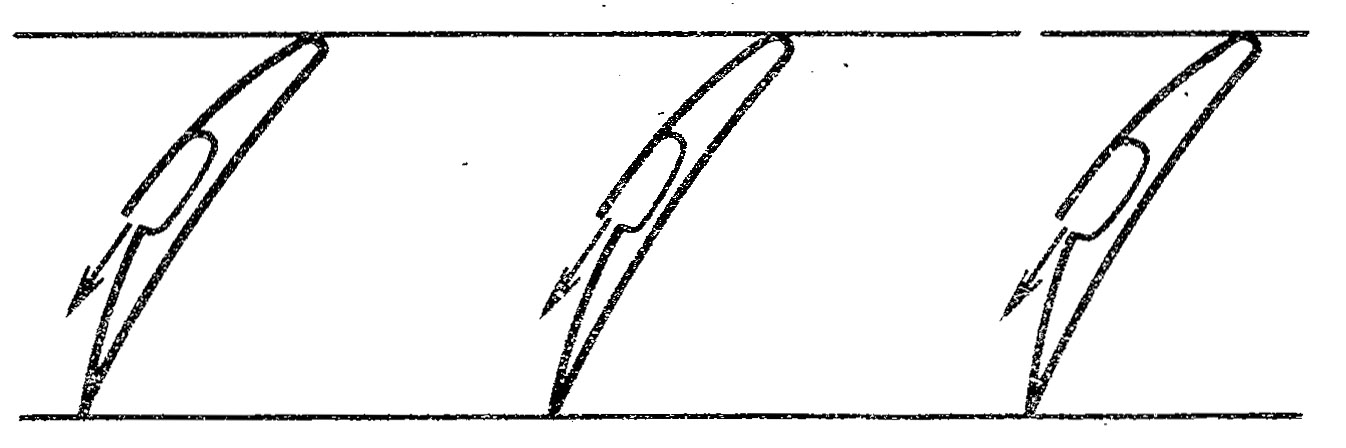
\includegraphics[width=8cm,keepaspectratio]{images/tereshenko1988a}}
	\hfill
	\subcaptionbox{отсос пограничного слоя}{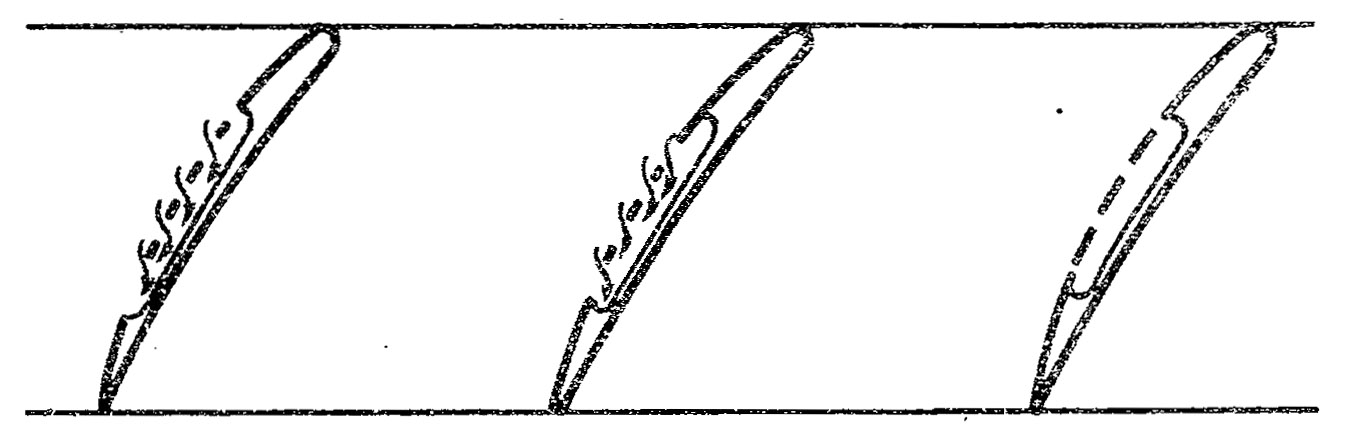
\includegraphics[width=8cm,keepaspectratio]{images/tereshenko1988b}}
\hfill
	\subcaptionbox{многорядные решётки}{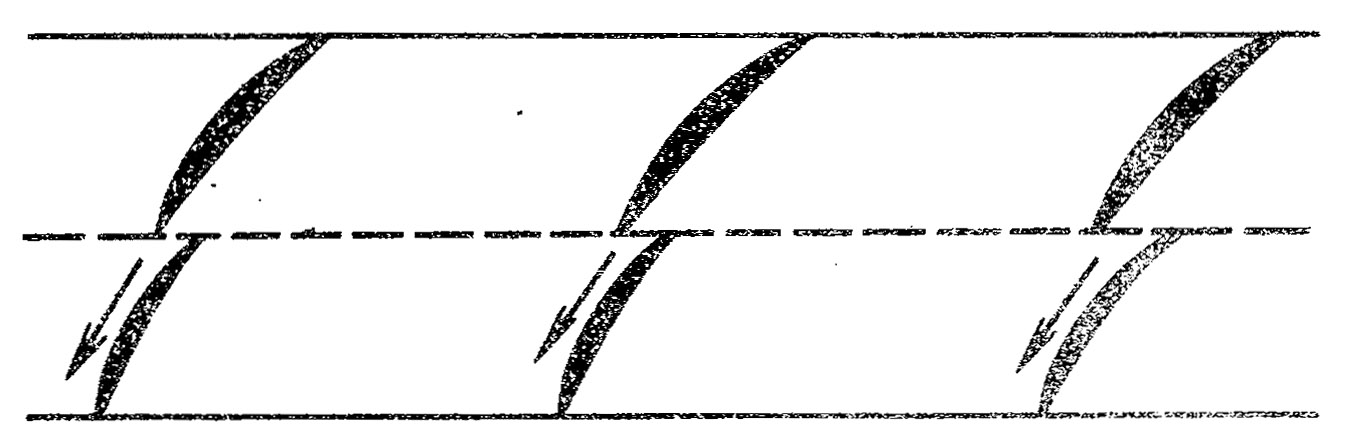
\includegraphics[width=8cm,keepaspectratio]{images/tereshenko1988c}}
\hfill
	\subcaptionbox{профили с турбулизаторами}{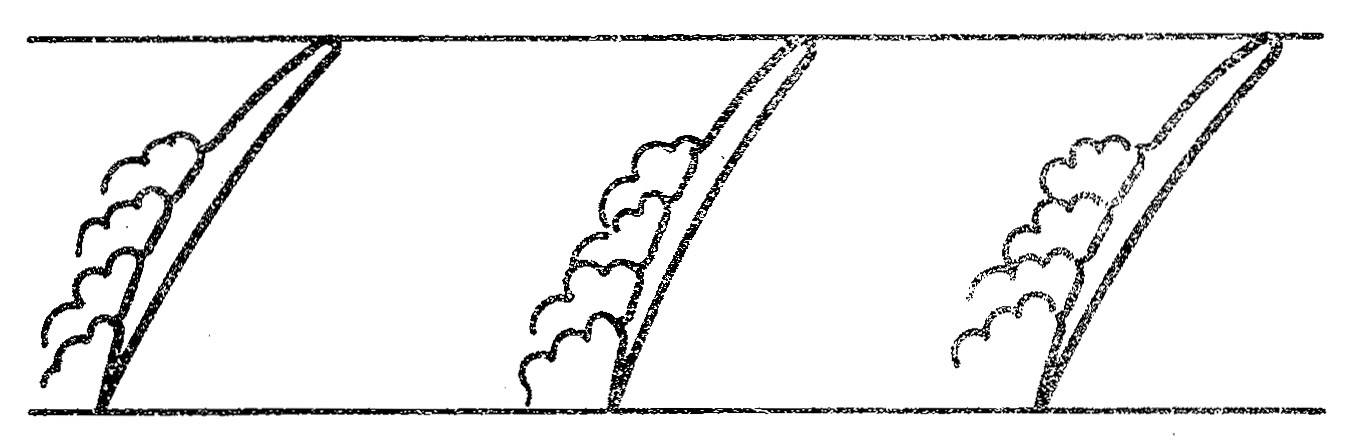
\includegraphics[width=8cm,keepaspectratio]{images/tereshenko1988d}}
}
\caption{Схемы управления обтеканием лопаток в решётках \cite{Tereschenko1988}}
\label{fig:Tereshenko1988}
\end{figure}

Активные методы управления пограничным слоем вдувом и отсосом газа с поверхности лопатки не нашли распространения в компрессорах и вентиляторах в связи с конструктивной сложностью. Наиболее простым методом является пассивный метод турбулизации потока, суть которого заключается в уменьшении участка ламинарного пограничного слоя на лопатке для снижения вероятности его отрыва. На рисунке \ref{fig:Tereschenko1988turb} сравнение степени повышения давления приведённой к расчётной \(\bar{\pi}_\text{ст}\) в ступени с гладкими лопатками и турбулизаторами потока в зависимости от приведённого расхода \(\bar{G}\) для разных приведённых частот вращения \(\bar{n}\). Применение турбулизатора позволило расширить область работы в сторону меньших расходов, но заметно снизило \(\bar{\pi}_\text{ст}\).
\begin{figure} [ht]
	\centerfloat{
		%\includegraphics[width=8cm,keepaspectratio]{images/tereshenko1988turb},
		% GNUPLOT: LaTeX picture with Postscript
\begingroup
  \makeatletter
  \providecommand\color[2][]{%
    \GenericError{(gnuplot) \space\space\space\@spaces}{%
      Package color not loaded in conjunction with
      terminal option `colourtext'%
    }{See the gnuplot documentation for explanation.%
    }{Either use 'blacktext' in gnuplot or load the package
      color.sty in LaTeX.}%
    \renewcommand\color[2][]{}%
  }%
  \providecommand\includegraphics[2][]{%
    \GenericError{(gnuplot) \space\space\space\@spaces}{%
      Package graphicx or graphics not loaded%
    }{See the gnuplot documentation for explanation.%
    }{The gnuplot epslatex terminal needs graphicx.sty or graphics.sty.}%
    \renewcommand\includegraphics[2][]{}%
  }%
  \providecommand\rotatebox[2]{#2}%
  \@ifundefined{ifGPcolor}{%
    \newif\ifGPcolor
    \GPcolorfalse
  }{}%
  \@ifundefined{ifGPblacktext}{%
    \newif\ifGPblacktext
    \GPblacktexttrue
  }{}%
  % define a \g@addto@macro without @ in the name:
  \let\gplgaddtomacro\g@addto@macro
  % define empty templates for all commands taking text:
  \gdef\gplbacktext{}%
  \gdef\gplfronttext{}%
  \makeatother
  \ifGPblacktext
    % no textcolor at all
    \def\colorrgb#1{}%
    \def\colorgray#1{}%
  \else
    % gray or color?
    \ifGPcolor
      \def\colorrgb#1{\color[rgb]{#1}}%
      \def\colorgray#1{\color[gray]{#1}}%
      \expandafter\def\csname LTw\endcsname{\color{white}}%
      \expandafter\def\csname LTb\endcsname{\color{black}}%
      \expandafter\def\csname LTa\endcsname{\color{black}}%
      \expandafter\def\csname LT0\endcsname{\color[rgb]{1,0,0}}%
      \expandafter\def\csname LT1\endcsname{\color[rgb]{0,1,0}}%
      \expandafter\def\csname LT2\endcsname{\color[rgb]{0,0,1}}%
      \expandafter\def\csname LT3\endcsname{\color[rgb]{1,0,1}}%
      \expandafter\def\csname LT4\endcsname{\color[rgb]{0,1,1}}%
      \expandafter\def\csname LT5\endcsname{\color[rgb]{1,1,0}}%
      \expandafter\def\csname LT6\endcsname{\color[rgb]{0,0,0}}%
      \expandafter\def\csname LT7\endcsname{\color[rgb]{1,0.3,0}}%
      \expandafter\def\csname LT8\endcsname{\color[rgb]{0.5,0.5,0.5}}%
    \else
      % gray
      \def\colorrgb#1{\color{black}}%
      \def\colorgray#1{\color[gray]{#1}}%
      \expandafter\def\csname LTw\endcsname{\color{white}}%
      \expandafter\def\csname LTb\endcsname{\color{black}}%
      \expandafter\def\csname LTa\endcsname{\color{black}}%
      \expandafter\def\csname LT0\endcsname{\color{black}}%
      \expandafter\def\csname LT1\endcsname{\color{black}}%
      \expandafter\def\csname LT2\endcsname{\color{black}}%
      \expandafter\def\csname LT3\endcsname{\color{black}}%
      \expandafter\def\csname LT4\endcsname{\color{black}}%
      \expandafter\def\csname LT5\endcsname{\color{black}}%
      \expandafter\def\csname LT6\endcsname{\color{black}}%
      \expandafter\def\csname LT7\endcsname{\color{black}}%
      \expandafter\def\csname LT8\endcsname{\color{black}}%
    \fi
  \fi
    \setlength{\unitlength}{0.0500bp}%
    \ifx\gptboxheight\undefined%
      \newlength{\gptboxheight}%
      \newlength{\gptboxwidth}%
      \newsavebox{\gptboxtext}%
    \fi%
    \setlength{\fboxrule}{0.5pt}%
    \setlength{\fboxsep}{1pt}%
    \definecolor{tbcol}{rgb}{1,1,1}%
\begin{picture}(6802.00,5102.00)%
    \gplgaddtomacro\gplbacktext{%
      \csname LTb\endcsname%%
      \put(1036,1456){\makebox(0,0)[r]{\strut{}$0,6$}}%
      \csname LTb\endcsname%%
      \put(1036,2129){\makebox(0,0)[r]{\strut{}$0,7$}}%
      \csname LTb\endcsname%%
      \put(1036,2802){\makebox(0,0)[r]{\strut{}$0,8$}}%
      \csname LTb\endcsname%%
      \put(1036,3475){\makebox(0,0)[r]{\strut{}$0,9$}}%
      \csname LTb\endcsname%%
      \put(1036,4148){\makebox(0,0)[r]{\strut{}$1$}}%
      \csname LTb\endcsname%%
      \put(1036,4821){\makebox(0,0)[r]{\strut{}$1,1$}}%
      \csname LTb\endcsname%%
      \put(1204,1176){\makebox(0,0){\strut{}$0,4$}}%
      \csname LTb\endcsname%%
      \put(1841,1176){\makebox(0,0){\strut{}$0,5$}}%
      \csname LTb\endcsname%%
      \put(2477,1176){\makebox(0,0){\strut{}$0,6$}}%
      \csname LTb\endcsname%%
      \put(3114,1176){\makebox(0,0){\strut{}$0,7$}}%
      \csname LTb\endcsname%%
      \put(3750,1176){\makebox(0,0){\strut{}$0,8$}}%
      \csname LTb\endcsname%%
      \put(4387,1176){\makebox(0,0){\strut{}$0,9$}}%
      \csname LTb\endcsname%%
      \put(5024,1176){\makebox(0,0){\strut{}$1$}}%
      \csname LTb\endcsname%%
      \put(5660,1176){\makebox(0,0){\strut{}$1,1$}}%
      \csname LTb\endcsname%%
      \put(6297,1176){\makebox(0,0){\strut{}$1,2$}}%
    }%
    \gplgaddtomacro\gplfronttext{%
      \csname LTb\endcsname%%
      \put(266,3138){\rotatebox{-270}{\makebox(0,0){\strut{}$\bar{\pi}_\text{ст}$}}}%
      \put(3750,756){\makebox(0,0){\strut{}$\bar{G}$}}%
      \csname LTb\endcsname%%
      \put(5226,483){\makebox(0,0)[r]{\strut{}гладкие лопатки}}%
      \csname LTb\endcsname%%
      \put(5226,203){\makebox(0,0)[r]{\strut{}турбулизаторы}}%
      \put(70mm,44mm){\makebox(0,0)[l]{\strut{}$\bar{n} = 0.69$}}%
      \put(78mm,63mm){\makebox(0,0)[l]{\strut{}$\bar{n} = 0,82$}}%
      \put(88mm,78mm){\makebox(0,0)[l]{\strut{}$\bar{n} = 1,00$}}%
    }%
    \gplbacktext
    \put(0,0){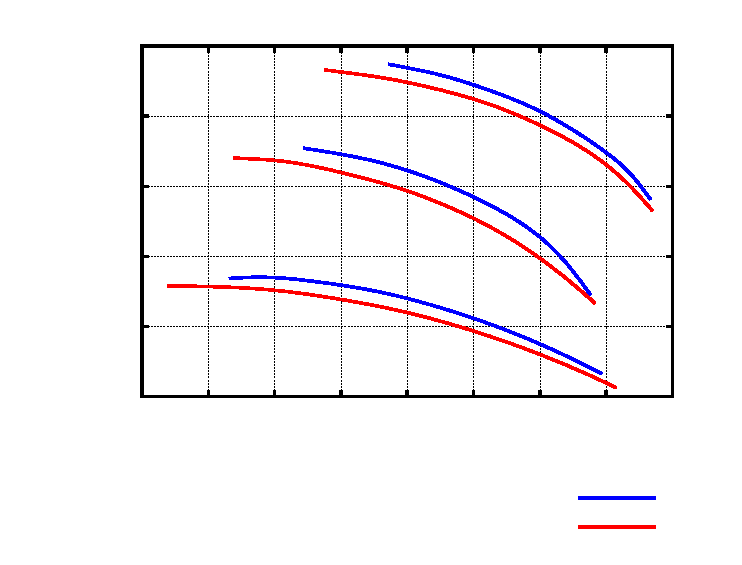
\includegraphics[width={340.10bp},height={255.10bp}]{teresch1988turb}}%
    \gplfronttext
  \end{picture}%
\endgroup

	}
	\caption{Характеристика ступени осевого компрессора с турбулизаторами на входном участке лопаток рабочего колеса \cite{Tereschenko1988}}
	\label{fig:Tereschenko1988turb}
\end{figure}

Применение многорядных решёток лопаток \cite{Tereschenko2015,Qiushi2010,LIU2022,Bammert1980,McGlumphy2009,VanEck2023,Wennerstrom1990} выглядит перспективным для применения в вентиляторных и компрессорных ступенях, так как характеристики подобных плоских решёток свидетельствуют о возможности получения большего поворота потока при меньших потерях полного давления. 

Экспериментальное исследование модели относительно высоконагруженной ступени (расчётный \(\Ht\) равен 0,45) \cite{LIU2022} продемонстрировали преимущество ступеней с двухрядными венцами РК и СА перед ступенями с однорядными венцами при расходе меньшем расчётного. Ступень из двухрядных решёток имела больший запас до срыва (рисунок \ref{fig:LIU2022}). Однако измеренный КПД на расчётном режиме оказался всего на 0,6\% выше чем у исходной ступени.
\begin{figure}[ht]
	\centerfloat{
% GNUPLOT: LaTeX picture with Postscript
\begingroup
  \makeatletter
  \providecommand\color[2][]{%
    \GenericError{(gnuplot) \space\space\space\@spaces}{%
      Package color not loaded in conjunction with
      terminal option `colourtext'%
    }{See the gnuplot documentation for explanation.%
    }{Either use 'blacktext' in gnuplot or load the package
      color.sty in LaTeX.}%
    \renewcommand\color[2][]{}%
  }%
  \providecommand\includegraphics[2][]{%
    \GenericError{(gnuplot) \space\space\space\@spaces}{%
      Package graphicx or graphics not loaded%
    }{See the gnuplot documentation for explanation.%
    }{The gnuplot epslatex terminal needs graphicx.sty or graphics.sty.}%
    \renewcommand\includegraphics[2][]{}%
  }%
  \providecommand\rotatebox[2]{#2}%
  \@ifundefined{ifGPcolor}{%
    \newif\ifGPcolor
    \GPcolorfalse
  }{}%
  \@ifundefined{ifGPblacktext}{%
    \newif\ifGPblacktext
    \GPblacktexttrue
  }{}%
  % define a \g@addto@macro without @ in the name:
  \let\gplgaddtomacro\g@addto@macro
  % define empty templates for all commands taking text:
  \gdef\gplbacktext{}%
  \gdef\gplfronttext{}%
  \makeatother
  \ifGPblacktext
    % no textcolor at all
    \def\colorrgb#1{}%
    \def\colorgray#1{}%
  \else
    % gray or color?
    \ifGPcolor
      \def\colorrgb#1{\color[rgb]{#1}}%
      \def\colorgray#1{\color[gray]{#1}}%
      \expandafter\def\csname LTw\endcsname{\color{white}}%
      \expandafter\def\csname LTb\endcsname{\color{black}}%
      \expandafter\def\csname LTa\endcsname{\color{black}}%
      \expandafter\def\csname LT0\endcsname{\color[rgb]{1,0,0}}%
      \expandafter\def\csname LT1\endcsname{\color[rgb]{0,1,0}}%
      \expandafter\def\csname LT2\endcsname{\color[rgb]{0,0,1}}%
      \expandafter\def\csname LT3\endcsname{\color[rgb]{1,0,1}}%
      \expandafter\def\csname LT4\endcsname{\color[rgb]{0,1,1}}%
      \expandafter\def\csname LT5\endcsname{\color[rgb]{1,1,0}}%
      \expandafter\def\csname LT6\endcsname{\color[rgb]{0,0,0}}%
      \expandafter\def\csname LT7\endcsname{\color[rgb]{1,0.3,0}}%
      \expandafter\def\csname LT8\endcsname{\color[rgb]{0.5,0.5,0.5}}%
    \else
      % gray
      \def\colorrgb#1{\color{black}}%
      \def\colorgray#1{\color[gray]{#1}}%
      \expandafter\def\csname LTw\endcsname{\color{white}}%
      \expandafter\def\csname LTb\endcsname{\color{black}}%
      \expandafter\def\csname LTa\endcsname{\color{black}}%
      \expandafter\def\csname LT0\endcsname{\color{black}}%
      \expandafter\def\csname LT1\endcsname{\color{black}}%
      \expandafter\def\csname LT2\endcsname{\color{black}}%
      \expandafter\def\csname LT3\endcsname{\color{black}}%
      \expandafter\def\csname LT4\endcsname{\color{black}}%
      \expandafter\def\csname LT5\endcsname{\color{black}}%
      \expandafter\def\csname LT6\endcsname{\color{black}}%
      \expandafter\def\csname LT7\endcsname{\color{black}}%
      \expandafter\def\csname LT8\endcsname{\color{black}}%
    \fi
  \fi
    \setlength{\unitlength}{0.0500bp}%
    \ifx\gptboxheight\undefined%
      \newlength{\gptboxheight}%
      \newlength{\gptboxwidth}%
      \newsavebox{\gptboxtext}%
    \fi%
    \setlength{\fboxrule}{0.5pt}%
    \setlength{\fboxsep}{1pt}%
    \definecolor{tbcol}{rgb}{1,1,1}%
\begin{picture}(6802.00,5102.00)%
    \gplgaddtomacro\gplbacktext{%
      \csname LTb\endcsname%%
      \put(1204,2016){\makebox(0,0)[r]{\strut{}$0,35$}}%
      \csname LTb\endcsname%%
      \put(1204,2717){\makebox(0,0)[r]{\strut{}$0,4$}}%
      \csname LTb\endcsname%%
      \put(1204,3419){\makebox(0,0)[r]{\strut{}$0,45$}}%
      \csname LTb\endcsname%%
      \put(1204,4120){\makebox(0,0)[r]{\strut{}$0,5$}}%
      \csname LTb\endcsname%%
      \put(1204,4821){\makebox(0,0)[r]{\strut{}$0,55$}}%
      \csname LTb\endcsname%%
      \put(1372,1736){\makebox(0,0){\strut{}$0,4$}}%
      \csname LTb\endcsname%%
      \put(1978,1736){\makebox(0,0){\strut{}$0,45$}}%
      \csname LTb\endcsname%%
      \put(2584,1736){\makebox(0,0){\strut{}$0,5$}}%
      \csname LTb\endcsname%%
      \put(3191,1736){\makebox(0,0){\strut{}$0,55$}}%
      \csname LTb\endcsname%%
      \put(3797,1736){\makebox(0,0){\strut{}$0,6$}}%
      \csname LTb\endcsname%%
      \put(4403,1736){\makebox(0,0){\strut{}$0,65$}}%
      \csname LTb\endcsname%%
      \put(5009,1736){\makebox(0,0){\strut{}$0,7$}}%
      \put(5177,2016){\makebox(0,0)[l]{\strut{}$0,75$}}%
      \put(5177,2717){\makebox(0,0)[l]{\strut{}$0,8$}}%
      \put(5177,3419){\makebox(0,0)[l]{\strut{}$0,85$}}%
      \put(5177,4120){\makebox(0,0)[l]{\strut{}$0,9$}}%
      \put(5177,4821){\makebox(0,0)[l]{\strut{}$0,95$}}%
    }%
    \gplgaddtomacro\gplfronttext{%
      \csname LTb\endcsname%%
      \put(266,3418){\rotatebox{-270}{\makebox(0,0){\strut{}$\Ht$}}}%
      \put(6157,3418){\rotatebox{-270}{\makebox(0,0){\strut{}$\eta$}}}%
      \put(3190,1316){\makebox(0,0){\strut{}$\ca$}}%
      \csname LTb\endcsname%%
      \put(3938,1043){\makebox(0,0)[r]{\strut{}$\Ht$ двухрядный}}%
      \csname LTb\endcsname%%
      \put(3938,763){\makebox(0,0)[r]{\strut{}$\Ht$ однорядный}}%
      \csname LTb\endcsname%%
      \put(3938,483){\makebox(0,0)[r]{\strut{}$\eta$ двухрядный}}%
      \csname LTb\endcsname%%
      \put(3938,203){\makebox(0,0)[r]{\strut{}$\eta$ однорядный}}%
    }%
    \gplbacktext
    \put(0,0){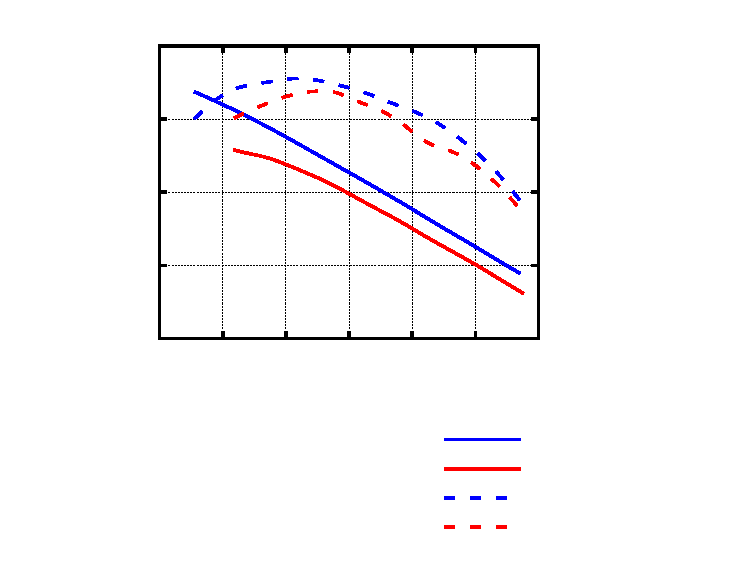
\includegraphics[width={340.10bp},height={255.10bp}]{LIU2022}}%
    \gplfronttext
  \end{picture}%
\endgroup

	}
	\caption{Сравнение характеристик ступени с двухрядными и однорядными венцами \cite{LIU2022}}
	\label{fig:LIU2022}
\end{figure}

Градиент давления при течении в проточной части можно скомпенсировать, плавно увеличивая скорости потока вдоль течения, за счет уменьшения сечения проточной части от входа к выходу из вентилятора. Такие вентиляторы называются вентиляторами с меридиональным ускорением потока. Уменьшение сечения проточной части, как правило, обеспечивается плавным увеличением относительного диаметра втулки \(\bar{d}\) (рисунок \ref{fig:schemaMrdnl}). Характеристикой течения в проточной части с меридиональным ускорением потока является отношение осевых плотностей тока на входе (1) и выходе (2) из решётки (Axial velocity density ratio) \(AVDR = \rho_2 C_\text{2a}/\rho_1 C_\text{1a}\). Для несжимаемого газа, соответственно, коэффициент меридионального ускорения \(m = C_\text{2a}/C_\text{1a}\). 
\begin{figure}[ht]
	\centerfloat{
		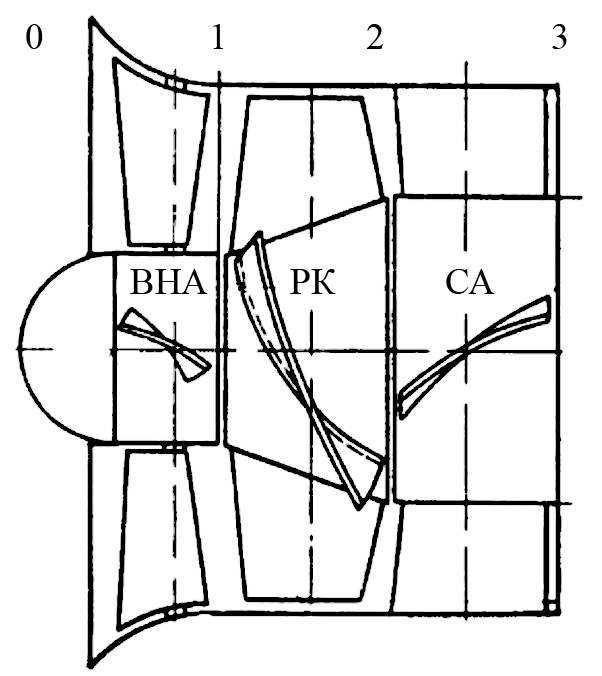
\includegraphics[width=8cm,keepaspectratio]{images/schemaMrdnl}
	}
	\caption{Схема вентилятора с меридиональным ускорением потока \cite{Brusilovskiy2004}}
	\label{fig:schemaMrdnl}
\end{figure}

При отношении осевых скоростей при входе и выходе из решётки больше 1, то есть при ускорении потока, пограничные слои на элементах проточной части вентилятора должны становиться тоньше, отрыв потока должен затягиваться, а потери полного давления снижаться. По результатам работы \cite{SenthilKumaran2015} по исследованию влияния \(AVDR\) на характеристики компрессорной ступени было установлено, что увеличение \(AVDR\) способствует росту КПД ступени до некоторого предельного значения, после которого увеличение \(AVDR\) уже не приводит к заметным изменениям. 
 
Снижение диффузорности течения позволяет получить эффективные вентиляторы в области параметров, выходящей за границы значений параметров типичных для эффективной осевой ступени с цилиндрической проточной частью \cite{Eck1972}. Спроектированный на сравнительно большое значение коэффициента теоретического напора \(\Ht\) равном 0,52 при коэффициенте расхода в сечении за рабочим колесом \(\bar{c}_\text{2a}\) равном 0,55 вентилятор \cite{Brusilovskiy1962} показал достаточно высокий КПД равный 0,865 и хорошее регулирование поворотом лопаток входного направляющего аппарата. Максимальное значение приведённого напора \(\bar{H}\) при регулировании составило примерно 0,6. Меридиональное ускорение потока происходило по большей части в рабочем колесе, где относительный диаметр втулки \(\bar{d}\)  менялся от 0,545 перед рабочим колесом до 0,7 перед спрямляющим аппаратом. Спрямляющий аппарат был выполнен с цилиндрической проточной частью. Степень реактивности на среднем радиусе составила 0,74.

Большое экспериментальное исследование вентиляторов с меридиональным ускорением потока предназначенных для местного проветривания в шахтах было проведено С.~К.~Ивановым \cite{Ivanov1969}. В результате исследований были спроектированы схемы вентиляторов с меридиональным ускорением потока в рабочем колесе, подходящие по требованиям для местного проветривания шахт. Они сочетают уровень коэффициента напора \(\bar{H}\) от 0,35 до 0,4 при коэффициентах расхода \(\bar{c}_\text{2a}\) от 0,4 до 0,6, максимальные КПД \(\eta\) от 0,85 до 0,87, при этом обладая хорошей регулируемостью поворотом входного направляющего аппарата.

Большие значения \(\Ht\) ступеней характерны для авиационных двигателей. Уменьшение удельного веса и повышение количества полезной подведённой энергии критичны для авиационной техники в целом. В вентиляторных ступенях авиационных газотурбинных двигателей (ГТД) в связи с относительно малой величиной втулки \(\bar{d}\) и высоким коэффициентом напора \(\bar{H}\) велик риск наступления срыва потока \cite{Kazandjan1983}. Для предотвращения срыва потока и повышения напора обеспечивается ускорение осевой компоненты скорости в межлопаточных каналах.

%Развитие рынка микро-ГТД интенсифицирует развитие диагональных ступеней компрессоров \cite{Cevik2009, Kock2017,VanEck2023}, во многом близких к осевым вентиляторам с меридиональным ускорением потока. Такие ступени применительно в микро-ГТД имеют меньшие радиальные габариты чем центробежные ступени и развивают больший коэффициент напора \(\bar{H}\) чем осевые ступени.

\section{Профилирование лопаток вентилятора с меридиональным ускорением}

Работа подводимая к рабочему телу в рабочем колесе \(H_\text{т}\), \(\si\joule/\si\kilogram\), турбомашины определяется кинематикой потока через уравнение Эйлера:
\begin{equation}
	H_\text{т} = U_2 C_{2u} - U_2 C_{1u},
	\label{eq:Ht}
\end{equation}
или в безразмерном виде (параграф \ref{sec:ch1/sec1}):
\begin{equation}
	\bar{H}_\text{т} = H_\text{т}/U_\text{к}^2 = \bar{r}_2 \bar{c}_{2u} - \bar{r}_1 \bar{c}_{1u},
	\label{eq:H_t}
\end{equation}
\begin{eqexpl}
	\item{\(U\)} окружная скорость колеса, \(\si\meter/\si\second\);
	\item{\(U_\text{к}\)} окружная скорость периферии колеса, \(\si\meter/\si\second\);
	\item{\(C_{u}\)} окружная компонента скорости потока, \(\si\meter/\si\second\);
	\item{\(\bar{c}_{u}\)} коэффициент окружной компоненты скорости потока, \(C_{u}/U\);
	\item{\(\bar{r}\)} приведённый радиус, \(r/R\);
	\item{\(R\)} радиус рабочего колеса, \(\si\meter\).
\end{eqexpl}
Задаваясь необходимым коэффициентом расхода \(\bar{c}_\text{a}\) коэффициент теоретического напора определяется только направлениями скоростей перед и за колесом:
\begin{equation}
	\bar{H}_\text{т} = \bar{r}_2 \bar{c}_\text{2a} \tan\alpha_2 - \bar{r}_1 \bar{c}_{1a} \tan\alpha_1,
	\label{eq:H_t_tan}
\end{equation}

Профилирование лопаток турбомашины подразумевает формирование геометрии лопаточных венцов, обеспечивающей необходимую кинематику потока, то есть обеспечение заданных направлений скоростей, давления и расхода. 

Течение в лопаточном венце сложно для описания –-- вторичные течения, нестационарность течения, взаимодействия пограничных слоёв на поверхностях лопаток и периферийных поверхностях, теплообмен, вибрация лопаток и т.д. При проектировании обычно используют математические модели, в значительной мере упрощающие действительное течение, начиная с того, что  считают течение установившимся.

\subsection{Профилирование лопаток цилиндрической ступени}\label{sec:ch1/profil}

 Традиционным упрощением при рассмотрении течения в осевой ступени является гипотеза плоских сечений, впервые высказанная Н.Е. Жуковским \cite{Joukovskiy1949}. Согласно этой гипотезе течение в проточной части можно разделить коаксиальными поверхностями на элементарные цилиндрические слои течения. При этом течения в соседних слоях в первом приближении независимы. Уравнение \ref{eq:H_t_tan} преобразуется к виду:
\begin{equation}
	\bar{H}_\text{т} = \bar{c}_\text{a} \left( \tan\alpha_2 - \tan\alpha_1 \right).
	\label{eq:H_t_cil}
\end{equation}
\begin{eqexpl}
	\item{$\alpha$} угол между скоростью потока в абсолютном движении и осью решётки.
\end{eqexpl}

Далее, каждый элементарный цилиндрический слой течения разворачивается на плоскость, образуя бесконечную решётку профилей. Рассматривая течение в этой плоскости в относительном движении, то есть в системе координат, в которой решётка остаётся неподвижной, разница в окружных компонентах скорости остаётся той же, что и в абсолютной системе координат: \(\Delta C_\text{u} = \Delta W_\text{u}\), соответственно \(\tan\alpha_2 - \tan\alpha_1 = \tan\beta_2 - \tan\beta_1\), где \(\beta\) "--- угол направления скорости в относительном движении. Течение газа в неподвижной плоской решётке профилей и определение величины \(\tan\beta_2 - \tan\beta_1\) сравнительно просто поддаётся теоретическому и экспериментальному исследованию. 

Данный подход, основанный на идеализированном двухмерном потоке, позволяет строить действующие машины с эксплуатационными параметрами близкими к расчётным. Гипотеза плоских сечений отражает основную суть явлений при обтекании лопаточных венцов турбомашин. Учёт остальных явлений проводится в процессе уточнения основного решения полученного на основе рассмотрения двухмерного течения в решётках профилей.

Для описания геометрии решёток и профиля используются следующие параметры (рисунок \ref{fig:cascad}).  
\begin{figure} [ht]
	\centerfloat{
		\includegraphics{images/cascad}
	}
	\caption{Основные геометрические параметры профиля и решётки профилей} 
	\label{fig:cascad}
\end{figure}
\eqexplSetIntro{}
\begin{eqexpl}
\item{\(c\)}  толщина профиля, максимальное расстояние между ближайшими точками корытца и спинки, \(\si\meter\); 
\item{\(b\)} хорда профиля, расстояние между крайними точками средней линии профиля, \(\si\meter\); 
\item{\(f\)} изгиб профиля, максимальное расстояние от средней линии до хорды профиля, \(\si\meter\);
\item{\(t\)} шаг решётки, расстояние между соответствующими точками соседних профилей, \(\si\meter\).
%\item{средняя линия профиля} геометрическое множество точек, не выходящее за контур профиля, минимальное расстояние от которых одинаково до линий корытца и спинки профиля.
\end{eqexpl}

Для характеристики профиля в решётке будем использовать относительные величины: 
\begin{eqexpl}
\item{\(\bar{c}\)} относительная толщина профиля, \(c/b\); 
\item{\(\bar{f}\)} относительный изгиб профиля, \(f/b\);
\item{\(\tau\)} густота решётки, \(b/t\).
\end{eqexpl}

Линия соединяющая соответствующие точки профилей называется фронтом решётки, а нормальная к ней – осью решётки. Углы, характеризующие расположение профилей в решётке, обозначаются следующим образом:
\begin{eqexpl}
\item{\(\theta_{\text{г}}\)} угол установки, угол между осью решетки и хордой профиля; 
\item{\(\beta_\text{л}\)} углы между касательными к средней линии профиля и осью решётки в точках передней (1) и задней кромки (2);
\item{\(\upsilon\)} угол изгиба профиля.
\end{eqexpl}
\eqexplSetIntro{где}

Задача определения геометрии решётки, обеспечивающей необходимую кинематику потока, является обратной задачей аэродинамики. Количество неизвестных в этой задаче меньше количества параметров, и заданную кинематику может обеспечить бесконечное число вариантов решёток профилей. Для невязкого несжимаемого течения угол атаки \(i\) и изгиб профиля \(\bar{f}\) являются практически эквивалентными способами обеспечить необходимую кинематику потока "--- для каждого \(i\) можно подобрать такой \(\bar{f}\), что будет обеспечен необходимый поворот потока. Однако в случае вязкого течения меньшие потери полного давления соответствуют течению в решётках с небольшими углами атаки. Все эти решётки будут отличаться по своим эксплуатационным характеристикам, таким как прочность, эффективность, диапазон эффективной работы. Для замыкания задачи профилирования задаются углом атаки \(i\) и густотой решётки \(\tau\), исходя из опыта проектирования машин различного назначения.

Авторы исследований по разному определяют значения номинального угла атаки, характеризуемого режимом работы решётки. Хауэлл \cite{Howell1945} считал, что угол атаки должен лежать в пределах от минус 5 до плюс 5 градусов. Либляйн \cite{Lieblein1959} принимал за номинальный угол атаки соответствующий минимуму потерь полного давления в решётке. 

А.\,П.\,Комаров \cite{Komarov1967} определил номинальный угол атаки, как соответствующий максимальному КПД решётки. На основании обработки большого количества экспериментальных продувок решёток профилей им была предложена приближенная формула для нахождения угла атаки, соответствующего максимальному КПД решётки:
\begin{equation}
	i_{\eta_\text{max}}=4,5-0,3\frac{\upsilon}{\tau} \left[ 1,81- \left(2\bar{x}_{f}\right)^2 \right],
\end{equation}
\begin{eqexpl}
	\item{\(\upsilon\)} угол изгиба профиля, \(\si\degree\);
	\item{\(\bar{x}_f\)} относительное положение точки средней линии профиля с максимальным изгибом;
\end{eqexpl}

В работе \cite{Emery1951} номинальным углом атаки принят тот при котором реализуется плавное распределение профиля давления на контуре лопатки. Угол атаки соответствующий безударному входу, при котором точка торможения потока располагается на передней кромке был принят в качестве номинального в работе \cite{Judin1947}. В работе \cite{Brusilovskiy1986}, для учета действия центробежных сил на течение во вращающихся решётках профилей, рекомендуется для периферии рабочего колеса вентилятора выбирать  небольшие отрицательные величины углов атаки от минус 2 до минус 3, а для привтулочных сечений от плюс 2 до плюс 4.

Работа совершённая над рабочем телом рабочим колесом должна быть достаточна для работы при меньших скоростях в целях обеспечения необходимой механического прочности лопаточного венца и снижения уровня шума, но, при этом, аэродинамическая нагруженность недостаточна для образования отрыва потока и работе с низкой эффективностью. Аэродинамическая нагруженность при небольших углах атаки \(i\) в большой степени зависит от густоты решётки \(\tau\). Подход к выбору рационального значения \(\tau\) во многих исследованиях различен. С.\,А.\,Довжик \cite{Dovjik1968} при значениях коэффициента теоретической работы \(\Ht\) не более 0,3, исходя из опыта проектирования компрессоров, рекомендует значения \(\tau\) на среднем радиусе от 1,0 до 1,2. Хауэлл \cite{Howell1945} для своего номинального режима работы рекомендует для определения рационального значения \(\tau\) зависимость от направления потока показанную на рисунке \ref{fig:tauRek}. В работе \cite{Bunimovich1967} А.\,И.\,Бунимовичем и А.\,А.\,Святогоровым проведено экспериментальное исследование характеристик плоских компрессорных решёток профилей и обобщение его результатов. Одним из результатов работы стали рекомендации по выбору оптимальной густоты решётки (рисунок \ref{fig:tauRek}). Для концевых сечений рекомендуемые густоты и углы атаки отличаются от выбранных по продувкам плоских решёток \cite{Brusilovskiy1975b}.
\begin{figure} [ht]
	\centerfloat{
		% GNUPLOT: LaTeX picture with Postscript
\begingroup
  \makeatletter
  \providecommand\color[2][]{%
    \GenericError{(gnuplot) \space\space\space\@spaces}{%
      Package color not loaded in conjunction with
      terminal option `colourtext'%
    }{See the gnuplot documentation for explanation.%
    }{Either use 'blacktext' in gnuplot or load the package
      color.sty in LaTeX.}%
    \renewcommand\color[2][]{}%
  }%
  \providecommand\includegraphics[2][]{%
    \GenericError{(gnuplot) \space\space\space\@spaces}{%
      Package graphicx or graphics not loaded%
    }{See the gnuplot documentation for explanation.%
    }{The gnuplot epslatex terminal needs graphicx.sty or graphics.sty.}%
    \renewcommand\includegraphics[2][]{}%
  }%
  \providecommand\rotatebox[2]{#2}%
  \@ifundefined{ifGPcolor}{%
    \newif\ifGPcolor
    \GPcolorfalse
  }{}%
  \@ifundefined{ifGPblacktext}{%
    \newif\ifGPblacktext
    \GPblacktexttrue
  }{}%
  % define a \g@addto@macro without @ in the name:
  \let\gplgaddtomacro\g@addto@macro
  % define empty templates for all commands taking text:
  \gdef\gplbacktext{}%
  \gdef\gplfronttext{}%
  \makeatother
  \ifGPblacktext
    % no textcolor at all
    \def\colorrgb#1{}%
    \def\colorgray#1{}%
  \else
    % gray or color?
    \ifGPcolor
      \def\colorrgb#1{\color[rgb]{#1}}%
      \def\colorgray#1{\color[gray]{#1}}%
      \expandafter\def\csname LTw\endcsname{\color{white}}%
      \expandafter\def\csname LTb\endcsname{\color{black}}%
      \expandafter\def\csname LTa\endcsname{\color{black}}%
      \expandafter\def\csname LT0\endcsname{\color[rgb]{1,0,0}}%
      \expandafter\def\csname LT1\endcsname{\color[rgb]{0,1,0}}%
      \expandafter\def\csname LT2\endcsname{\color[rgb]{0,0,1}}%
      \expandafter\def\csname LT3\endcsname{\color[rgb]{1,0,1}}%
      \expandafter\def\csname LT4\endcsname{\color[rgb]{0,1,1}}%
      \expandafter\def\csname LT5\endcsname{\color[rgb]{1,1,0}}%
      \expandafter\def\csname LT6\endcsname{\color[rgb]{0,0,0}}%
      \expandafter\def\csname LT7\endcsname{\color[rgb]{1,0.3,0}}%
      \expandafter\def\csname LT8\endcsname{\color[rgb]{0.5,0.5,0.5}}%
    \else
      % gray
      \def\colorrgb#1{\color{black}}%
      \def\colorgray#1{\color[gray]{#1}}%
      \expandafter\def\csname LTw\endcsname{\color{white}}%
      \expandafter\def\csname LTb\endcsname{\color{black}}%
      \expandafter\def\csname LTa\endcsname{\color{black}}%
      \expandafter\def\csname LT0\endcsname{\color{black}}%
      \expandafter\def\csname LT1\endcsname{\color{black}}%
      \expandafter\def\csname LT2\endcsname{\color{black}}%
      \expandafter\def\csname LT3\endcsname{\color{black}}%
      \expandafter\def\csname LT4\endcsname{\color{black}}%
      \expandafter\def\csname LT5\endcsname{\color{black}}%
      \expandafter\def\csname LT6\endcsname{\color{black}}%
      \expandafter\def\csname LT7\endcsname{\color{black}}%
      \expandafter\def\csname LT8\endcsname{\color{black}}%
    \fi
  \fi
    \setlength{\unitlength}{0.0500bp}%
    \ifx\gptboxheight\undefined%
      \newlength{\gptboxheight}%
      \newlength{\gptboxwidth}%
      \newsavebox{\gptboxtext}%
    \fi%
    \setlength{\fboxrule}{0.5pt}%
    \setlength{\fboxsep}{1pt}%
    \definecolor{tbcol}{rgb}{1,1,1}%
\begin{picture}(9070.00,6802.00)%
    \gplgaddtomacro\gplbacktext{%
      \csname LTb\endcsname%%
      \put(868,1456){\makebox(0,0)[r]{\strut{}$0$}}%
      \csname LTb\endcsname%%
      \put(868,2089){\makebox(0,0)[r]{\strut{}$10$}}%
      \csname LTb\endcsname%%
      \put(868,2722){\makebox(0,0)[r]{\strut{}$20$}}%
      \csname LTb\endcsname%%
      \put(868,3355){\makebox(0,0)[r]{\strut{}$30$}}%
      \csname LTb\endcsname%%
      \put(868,3989){\makebox(0,0)[r]{\strut{}$40$}}%
      \csname LTb\endcsname%%
      \put(868,4622){\makebox(0,0)[r]{\strut{}$50$}}%
      \csname LTb\endcsname%%
      \put(868,5255){\makebox(0,0)[r]{\strut{}$60$}}%
      \csname LTb\endcsname%%
      \put(868,5888){\makebox(0,0)[r]{\strut{}$70$}}%
      \csname LTb\endcsname%%
      \put(868,6521){\makebox(0,0)[r]{\strut{}$80$}}%
      \csname LTb\endcsname%%
      \put(1789,1176){\makebox(0,0){\strut{}$-20$}}%
      \csname LTb\endcsname%%
      \put(3295,1176){\makebox(0,0){\strut{}$0$}}%
      \csname LTb\endcsname%%
      \put(4801,1176){\makebox(0,0){\strut{}$20$}}%
      \csname LTb\endcsname%%
      \put(6306,1176){\makebox(0,0){\strut{}$40$}}%
      \csname LTb\endcsname%%
      \put(7812,1176){\makebox(0,0){\strut{}$60$}}%
    }%
    \gplgaddtomacro\gplfronttext{%
      \csname LTb\endcsname%%
      \put(266,3988){\rotatebox{-270}{\makebox(0,0){\strut{}$\Delta\beta, \si\degree$}}}%
      \put(4800,756){\makebox(0,0){\strut{}$\beta_2, \si\degree$}}%
      \csname LTb\endcsname%%
      \put(7494,483){\makebox(0,0)[r]{\strut{}Бунимович, Святогоров \cite{Bunimovich1967}}}%
      \csname LTb\endcsname%%
      \put(7494,203){\makebox(0,0)[r]{\strut{}Хауэлл \cite{Howell1945}}}%
    }%
    \gplbacktext
    \put(0,0){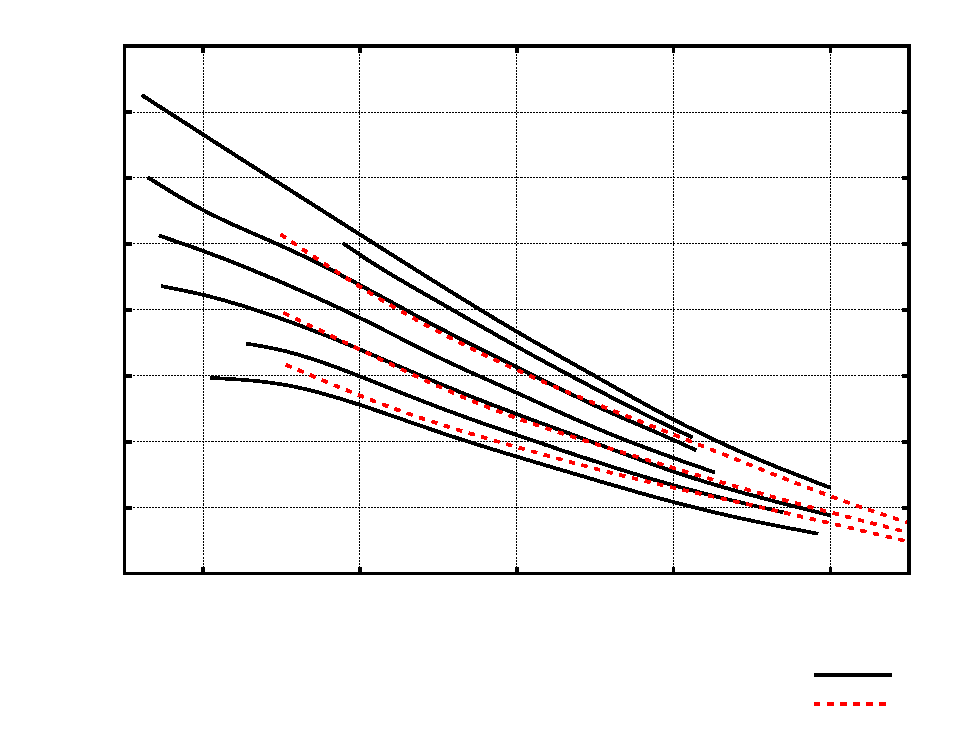
\includegraphics[width={453.50bp},height={340.10bp}]{BunSvjat}}%
    \gplfronttext
  \end{picture}%
\endgroup

	}
	\caption{Рекомендуемые значения густоты решётки \(\tau\) в зависимости от угла потока на выходе из решётки \(\beta_2\) и углом поворота потока \(\Delta\beta\)} 
	\label{fig:tauRek}
\end{figure}

После того как угол атаки \(i\) и густота решётки \(\tau\) определены, остаётся определить необходимый изгиб профиля \(\bar{f}\). Значение \(\bar{f}\) определяется либо из результатов обобщения экспериментальных продувок \cite{Emery1951,Bunimovich1967}, либо на основе теоретических характеристик \cite{Umnov1951,Uschakov1960,Bloch1961}, полученных при рассмотрении потенциального течения. 

Связь между направлением идеального потока перед и за решёткой профилей выражаются в виде зависимости \( \tan\beta_2 = A\tan\beta_1+B\), где \(A\) и \(B\) "--- коэффициенты характеризуемые геометрией решётки. Для определения \(A\) и \(B\) используются метод отображения \cite{Bloch1961}, или метод наложения потоков. В методе отображения используется течение в области которое можно посчитать. Течение в исследуемой области может быть изучено с помощью конформного преобразования. При использовании метода наложения потоков на контуре профиля располагается большое количество особенностей: вихрей, источников или диполей. Задача об определении характеристик решётки сводится к решению системы линейных алгебраических уравнений. 

Широкое распространение получил метод дискретных вихрей (МДВ) \cite{Belozerovskiy1978}. Бесконечная решётка профилей обтекается потенциальным невязким несжимаемым потоком. На контуре профиля расставляются точки дискретных вихрей и контрольные точки (рисунок \ref{fig:foilVortex}). В контрольных точках принимается, что поток касателен к контуру профиля. Необходимо задать критическую точку схода потока с профиля, в которой интенсивность вихря будет нулевой. На остальных профилях решётки вихри располагаются точно так же, как и на исходном профиле, образуя бесконечные цепочки вихрей. 

\begin{figure} [ht]
	\centerfloat{
		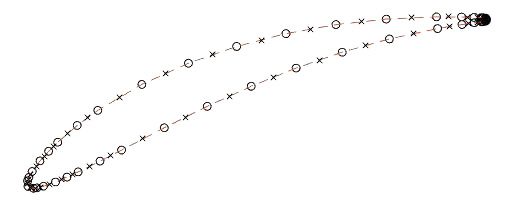
\includegraphics[width=8cm,keepaspectratio]{images/foilVortex} 
	} 
	\caption{Вихри \(\times\) и контрольные точки \(\circ\) на контуре профиля} 
	\label{fig:foilVortex}
\end{figure}

\subsection{Течение в вентиляторе с меридиональным ускорением}\label{sec:ch1/mrdnl}

При исследовании цилиндрических ступеней за прошедшее время было накоплено огромное количество экспериментальных данных и отработано большое число математических моделей. При любых изменениях в характере течения следует максимально полно использовать существующие модели и дополнять их по мере необходимости. Для моделирования течения и проектирования вентилятора с меридиональным ускорением потока, за основу берутся показавшие хорошие результаты модели течения в цилиндрической ступени.

Теория течения в меридиональном сечении развита в работах Ву \cite{Wu1952}, который предложил в качестве условных поверхностей тока поверхности \(S_1\) и \(S_2\) (рисунок \ref{fig:s1s2}). В качестве поверхности \(S_1\) принята традиционная поверхность от лопатки к лопатке. Поверхности тока \(S_2\) имеют радиальную форму перед лопатками, а в межлопаточном канале они изгибаются и скручиваются.

\begin{figure} [ht]
	\centerfloat{
		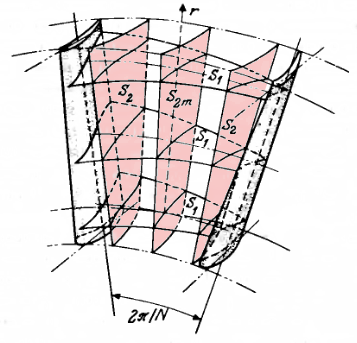
\includegraphics[width=8cm,keepaspectratio]{images/s1s2}
	}
	\caption{Поверхности тока \(S_1\) и \(S_2\) \cite{Wu1952}. \(S_2\) выделены красным} 
	\label{fig:s1s2}
\end{figure}

Следуя гипотезе плоских сечений, обычно пренебрегают скручиванием поверхностей \(S_1\). Их рассматривают, как образованные вращением от кривых линий тока в меридиональной плоскости вокруг оси турбомашины \cite{Sirotkin1972}. Параметры течения в межвенцовом зазоре определяются по углам наклона меридиональных линий и закону закрутки рабочего тела из уравнения радиального равновесия \cite{Smith1966} с помощью численных методов.

В осевых ступенях с умеренным отклонением поверхностей тока \(S_1\) от цилиндричности, не превышающей 15 градусов, используются методы теоретического анализа течения в лопаточных венцах для осевых турбомашин с цилиндрической проточной частью \cite{Sirotkin1972,Stepanov1962}, влиянием радиальной компоненты скорости при этом пренебрегают. 

Схема вентилятора с меридиональным ускорением подразумевает значительное увеличение коэффициента расхода в одной ступени и изменение радиуса линий тока в сечениях у втулки. Течение в таком лопаточном венце имеет выраженный трехмерный характер, определяемый значительной величиной радиальной составляющей скорости. Рассматривая невязкое безвихревое течение несжимаемого газа в решётке профилей на поверхностях \(S_1\), с помощью конформного отображения можно перейти к рассмотрению обтекания плоской решётки профилей в слое переменной толщины. 

При предварительном проектировании многоступенчатого компрессора, пользуются развёрткой на плоскость усечённого конуса (плоскость~\(W\))~\cite{Sachkova2000}: 
\begin{equation}
	W = r e^{i\varphi},
\end{equation}
\begin{eqexpl}
	\item{\(r, \phi\)} полярные координаты.
\end{eqexpl}

Отображение плоскости \(W\) на плоскость \(z\) с декартовыми координатами \(x\) и \(y\) проводится при помощи логарифмической функции 
\begin{equation}
z = \ln W,
\end{equation}
тогда координаты связанны выражениями:
\begin{equation}
	x = \ln r, y = \varphi.
\end{equation}

 В работе \cite{Nikitin1966} экспериментально изучено течение в диагональных решётках профилей, полученных таким отображением. Полученные характеристики  показали хорошее совпадение по величине отклонения потока в сравнении с исходной плоской решёткой профилей при безотрывном течении и различных числах Маха на входе в решётку \(M_1\) от 0,3 до 0,65. Использование продувок плоских профилей для определения характеристик диагональных решёток имеет недостаток "--- течение в пограничном слое вихревое и не переносится на исследуемую плоскость при конформных отображениях. Отображением можно пользоваться только при безотрывном течении и достаточно тонких пограничных слоях. На рисунке \ref{fig:nikitin} приводится сравнение распределения относительных  скоростей \(\bar{w} = w/W_1\) (где \(w\) "--- скорость на спинке, м/с; \(W_1\) "--- скорость перед решёткой, м/с)  на спинке лопатки, полученных экспериментально и пересчётом продувки соответствующей плоской решётки. Сравнение выполнено при трёх различных углах атаки и \(M_1\) приблизительно равном 0,5. При небольших отрицательных углах атаки имеет место хорошее совпадение, а по мере роста толщины пограничного слоя при увеличении угла атаки, отличия становятся существенными.
 
 \begin{figure} [ht]
 	\centerfloat{
 		%\includegraphics[width=8cm,keepaspectratio]{images/nikitin1966}
 		% GNUPLOT: LaTeX picture with Postscript
\begingroup
  \makeatletter
  \providecommand\color[2][]{%
    \GenericError{(gnuplot) \space\space\space\@spaces}{%
      Package color not loaded in conjunction with
      terminal option `colourtext'%
    }{See the gnuplot documentation for explanation.%
    }{Either use 'blacktext' in gnuplot or load the package
      color.sty in LaTeX.}%
    \renewcommand\color[2][]{}%
  }%
  \providecommand\includegraphics[2][]{%
    \GenericError{(gnuplot) \space\space\space\@spaces}{%
      Package graphicx or graphics not loaded%
    }{See the gnuplot documentation for explanation.%
    }{The gnuplot epslatex terminal needs graphicx.sty or graphics.sty.}%
    \renewcommand\includegraphics[2][]{}%
  }%
  \providecommand\rotatebox[2]{#2}%
  \@ifundefined{ifGPcolor}{%
    \newif\ifGPcolor
    \GPcolorfalse
  }{}%
  \@ifundefined{ifGPblacktext}{%
    \newif\ifGPblacktext
    \GPblacktexttrue
  }{}%
  % define a \g@addto@macro without @ in the name:
  \let\gplgaddtomacro\g@addto@macro
  % define empty templates for all commands taking text:
  \gdef\gplbacktext{}%
  \gdef\gplfronttext{}%
  \makeatother
  \ifGPblacktext
    % no textcolor at all
    \def\colorrgb#1{}%
    \def\colorgray#1{}%
  \else
    % gray or color?
    \ifGPcolor
      \def\colorrgb#1{\color[rgb]{#1}}%
      \def\colorgray#1{\color[gray]{#1}}%
      \expandafter\def\csname LTw\endcsname{\color{white}}%
      \expandafter\def\csname LTb\endcsname{\color{black}}%
      \expandafter\def\csname LTa\endcsname{\color{black}}%
      \expandafter\def\csname LT0\endcsname{\color[rgb]{1,0,0}}%
      \expandafter\def\csname LT1\endcsname{\color[rgb]{0,1,0}}%
      \expandafter\def\csname LT2\endcsname{\color[rgb]{0,0,1}}%
      \expandafter\def\csname LT3\endcsname{\color[rgb]{1,0,1}}%
      \expandafter\def\csname LT4\endcsname{\color[rgb]{0,1,1}}%
      \expandafter\def\csname LT5\endcsname{\color[rgb]{1,1,0}}%
      \expandafter\def\csname LT6\endcsname{\color[rgb]{0,0,0}}%
      \expandafter\def\csname LT7\endcsname{\color[rgb]{1,0.3,0}}%
      \expandafter\def\csname LT8\endcsname{\color[rgb]{0.5,0.5,0.5}}%
    \else
      % gray
      \def\colorrgb#1{\color{black}}%
      \def\colorgray#1{\color[gray]{#1}}%
      \expandafter\def\csname LTw\endcsname{\color{white}}%
      \expandafter\def\csname LTb\endcsname{\color{black}}%
      \expandafter\def\csname LTa\endcsname{\color{black}}%
      \expandafter\def\csname LT0\endcsname{\color{black}}%
      \expandafter\def\csname LT1\endcsname{\color{black}}%
      \expandafter\def\csname LT2\endcsname{\color{black}}%
      \expandafter\def\csname LT3\endcsname{\color{black}}%
      \expandafter\def\csname LT4\endcsname{\color{black}}%
      \expandafter\def\csname LT5\endcsname{\color{black}}%
      \expandafter\def\csname LT6\endcsname{\color{black}}%
      \expandafter\def\csname LT7\endcsname{\color{black}}%
      \expandafter\def\csname LT8\endcsname{\color{black}}%
    \fi
  \fi
    \setlength{\unitlength}{0.0500bp}%
    \ifx\gptboxheight\undefined%
      \newlength{\gptboxheight}%
      \newlength{\gptboxwidth}%
      \newsavebox{\gptboxtext}%
    \fi%
    \setlength{\fboxrule}{0.5pt}%
    \setlength{\fboxsep}{1pt}%
    \definecolor{tbcol}{rgb}{1,1,1}%
\begin{picture}(9070.00,2834.00)%
    \gplgaddtomacro\gplbacktext{%
      \csname LTb\endcsname%%
      \put(1036,560){\makebox(0,0)[r]{\strut{}$0,6$}}%
      \csname LTb\endcsname%%
      \put(1036,1197){\makebox(0,0)[r]{\strut{}$1$}}%
      \csname LTb\endcsname%%
      \put(1036,1993){\makebox(0,0)[r]{\strut{}$1,5$}}%
      \csname LTb\endcsname%%
      \put(1204,280){\makebox(0,0){\strut{}$0$}}%
      \csname LTb\endcsname%%
      \put(2676,280){\makebox(0,0){\strut{}$0,2$}}%
      \csname LTb\endcsname%%
      \put(4148,280){\makebox(0,0){\strut{}$0,4$}}%
      \csname LTb\endcsname%%
      \put(5621,280){\makebox(0,0){\strut{}$0,6$}}%
      \csname LTb\endcsname%%
      \put(7093,280){\makebox(0,0){\strut{}$0,8$}}%
      \csname LTb\endcsname%%
      \put(8565,280){\makebox(0,0){\strut{}$1$}}%
    }%
    \gplgaddtomacro\gplfronttext{%
      \csname LTb\endcsname%%
      \put(266,1276){\rotatebox{-270}{\makebox(0,0){\strut{}$\bar{w}$}}}%
      \csname LTb\endcsname%%
      \put(4884,2413){\makebox(0,0){\strut{}$ i = -5\si\degree $}}%
    }%
    \gplbacktext
    \put(0,0){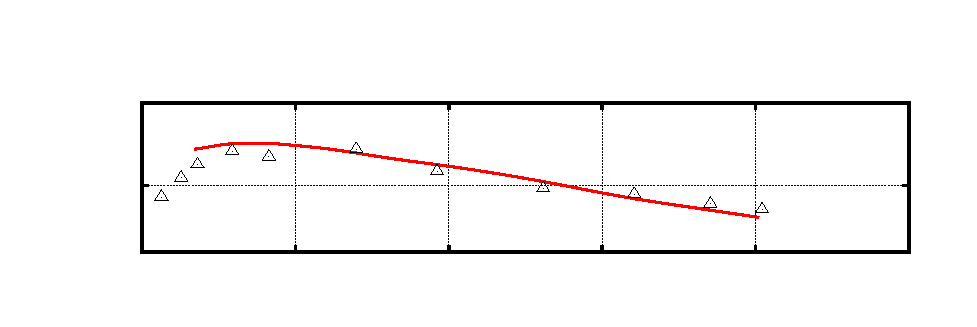
\includegraphics[width={453.50bp},height={141.70bp}]{nikitin1}}%
    \gplfronttext
  \end{picture}%
\endgroup
\\
 		% GNUPLOT: LaTeX picture with Postscript
\begingroup
  \makeatletter
  \providecommand\color[2][]{%
    \GenericError{(gnuplot) \space\space\space\@spaces}{%
      Package color not loaded in conjunction with
      terminal option `colourtext'%
    }{See the gnuplot documentation for explanation.%
    }{Either use 'blacktext' in gnuplot or load the package
      color.sty in LaTeX.}%
    \renewcommand\color[2][]{}%
  }%
  \providecommand\includegraphics[2][]{%
    \GenericError{(gnuplot) \space\space\space\@spaces}{%
      Package graphicx or graphics not loaded%
    }{See the gnuplot documentation for explanation.%
    }{The gnuplot epslatex terminal needs graphicx.sty or graphics.sty.}%
    \renewcommand\includegraphics[2][]{}%
  }%
  \providecommand\rotatebox[2]{#2}%
  \@ifundefined{ifGPcolor}{%
    \newif\ifGPcolor
    \GPcolorfalse
  }{}%
  \@ifundefined{ifGPblacktext}{%
    \newif\ifGPblacktext
    \GPblacktexttrue
  }{}%
  % define a \g@addto@macro without @ in the name:
  \let\gplgaddtomacro\g@addto@macro
  % define empty templates for all commands taking text:
  \gdef\gplbacktext{}%
  \gdef\gplfronttext{}%
  \makeatother
  \ifGPblacktext
    % no textcolor at all
    \def\colorrgb#1{}%
    \def\colorgray#1{}%
  \else
    % gray or color?
    \ifGPcolor
      \def\colorrgb#1{\color[rgb]{#1}}%
      \def\colorgray#1{\color[gray]{#1}}%
      \expandafter\def\csname LTw\endcsname{\color{white}}%
      \expandafter\def\csname LTb\endcsname{\color{black}}%
      \expandafter\def\csname LTa\endcsname{\color{black}}%
      \expandafter\def\csname LT0\endcsname{\color[rgb]{1,0,0}}%
      \expandafter\def\csname LT1\endcsname{\color[rgb]{0,1,0}}%
      \expandafter\def\csname LT2\endcsname{\color[rgb]{0,0,1}}%
      \expandafter\def\csname LT3\endcsname{\color[rgb]{1,0,1}}%
      \expandafter\def\csname LT4\endcsname{\color[rgb]{0,1,1}}%
      \expandafter\def\csname LT5\endcsname{\color[rgb]{1,1,0}}%
      \expandafter\def\csname LT6\endcsname{\color[rgb]{0,0,0}}%
      \expandafter\def\csname LT7\endcsname{\color[rgb]{1,0.3,0}}%
      \expandafter\def\csname LT8\endcsname{\color[rgb]{0.5,0.5,0.5}}%
    \else
      % gray
      \def\colorrgb#1{\color{black}}%
      \def\colorgray#1{\color[gray]{#1}}%
      \expandafter\def\csname LTw\endcsname{\color{white}}%
      \expandafter\def\csname LTb\endcsname{\color{black}}%
      \expandafter\def\csname LTa\endcsname{\color{black}}%
      \expandafter\def\csname LT0\endcsname{\color{black}}%
      \expandafter\def\csname LT1\endcsname{\color{black}}%
      \expandafter\def\csname LT2\endcsname{\color{black}}%
      \expandafter\def\csname LT3\endcsname{\color{black}}%
      \expandafter\def\csname LT4\endcsname{\color{black}}%
      \expandafter\def\csname LT5\endcsname{\color{black}}%
      \expandafter\def\csname LT6\endcsname{\color{black}}%
      \expandafter\def\csname LT7\endcsname{\color{black}}%
      \expandafter\def\csname LT8\endcsname{\color{black}}%
    \fi
  \fi
    \setlength{\unitlength}{0.0500bp}%
    \ifx\gptboxheight\undefined%
      \newlength{\gptboxheight}%
      \newlength{\gptboxwidth}%
      \newsavebox{\gptboxtext}%
    \fi%
    \setlength{\fboxrule}{0.5pt}%
    \setlength{\fboxsep}{1pt}%
    \definecolor{tbcol}{rgb}{1,1,1}%
\begin{picture}(9070.00,2834.00)%
    \gplgaddtomacro\gplbacktext{%
      \csname LTb\endcsname%%
      \put(1036,560){\makebox(0,0)[r]{\strut{}$0,6$}}%
      \csname LTb\endcsname%%
      \put(1036,1197){\makebox(0,0)[r]{\strut{}$1$}}%
      \csname LTb\endcsname%%
      \put(1036,1993){\makebox(0,0)[r]{\strut{}$1,5$}}%
      \csname LTb\endcsname%%
      \put(1204,280){\makebox(0,0){\strut{}$0$}}%
      \csname LTb\endcsname%%
      \put(2676,280){\makebox(0,0){\strut{}$0,2$}}%
      \csname LTb\endcsname%%
      \put(4148,280){\makebox(0,0){\strut{}$0,4$}}%
      \csname LTb\endcsname%%
      \put(5621,280){\makebox(0,0){\strut{}$0,6$}}%
      \csname LTb\endcsname%%
      \put(7093,280){\makebox(0,0){\strut{}$0,8$}}%
      \csname LTb\endcsname%%
      \put(8565,280){\makebox(0,0){\strut{}$1$}}%
    }%
    \gplgaddtomacro\gplfronttext{%
      \csname LTb\endcsname%%
      \put(266,1276){\rotatebox{-270}{\makebox(0,0){\strut{}$\bar{w}$}}}%
      \csname LTb\endcsname%%
      \put(4884,2413){\makebox(0,0){\strut{}$ i = 3\si\degree $}}%
    }%
    \gplbacktext
    \put(0,0){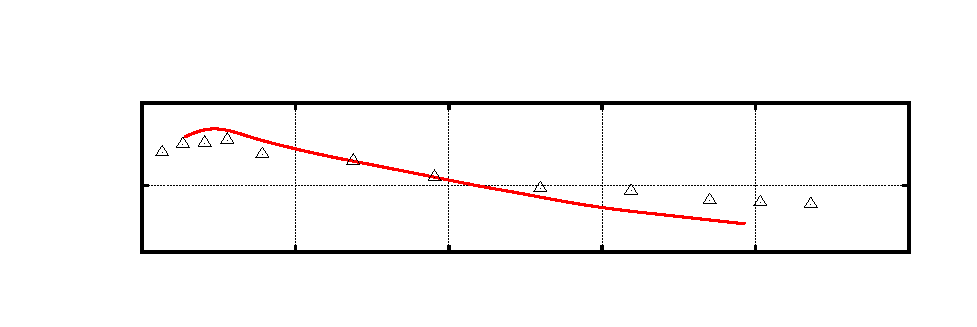
\includegraphics[width={453.50bp},height={141.70bp}]{nikitin2}}%
    \gplfronttext
  \end{picture}%
\endgroup
\\
 		% GNUPLOT: LaTeX picture with Postscript
\begingroup
  \makeatletter
  \providecommand\color[2][]{%
    \GenericError{(gnuplot) \space\space\space\@spaces}{%
      Package color not loaded in conjunction with
      terminal option `colourtext'%
    }{See the gnuplot documentation for explanation.%
    }{Either use 'blacktext' in gnuplot or load the package
      color.sty in LaTeX.}%
    \renewcommand\color[2][]{}%
  }%
  \providecommand\includegraphics[2][]{%
    \GenericError{(gnuplot) \space\space\space\@spaces}{%
      Package graphicx or graphics not loaded%
    }{See the gnuplot documentation for explanation.%
    }{The gnuplot epslatex terminal needs graphicx.sty or graphics.sty.}%
    \renewcommand\includegraphics[2][]{}%
  }%
  \providecommand\rotatebox[2]{#2}%
  \@ifundefined{ifGPcolor}{%
    \newif\ifGPcolor
    \GPcolorfalse
  }{}%
  \@ifundefined{ifGPblacktext}{%
    \newif\ifGPblacktext
    \GPblacktexttrue
  }{}%
  % define a \g@addto@macro without @ in the name:
  \let\gplgaddtomacro\g@addto@macro
  % define empty templates for all commands taking text:
  \gdef\gplbacktext{}%
  \gdef\gplfronttext{}%
  \makeatother
  \ifGPblacktext
    % no textcolor at all
    \def\colorrgb#1{}%
    \def\colorgray#1{}%
  \else
    % gray or color?
    \ifGPcolor
      \def\colorrgb#1{\color[rgb]{#1}}%
      \def\colorgray#1{\color[gray]{#1}}%
      \expandafter\def\csname LTw\endcsname{\color{white}}%
      \expandafter\def\csname LTb\endcsname{\color{black}}%
      \expandafter\def\csname LTa\endcsname{\color{black}}%
      \expandafter\def\csname LT0\endcsname{\color[rgb]{1,0,0}}%
      \expandafter\def\csname LT1\endcsname{\color[rgb]{0,1,0}}%
      \expandafter\def\csname LT2\endcsname{\color[rgb]{0,0,1}}%
      \expandafter\def\csname LT3\endcsname{\color[rgb]{1,0,1}}%
      \expandafter\def\csname LT4\endcsname{\color[rgb]{0,1,1}}%
      \expandafter\def\csname LT5\endcsname{\color[rgb]{1,1,0}}%
      \expandafter\def\csname LT6\endcsname{\color[rgb]{0,0,0}}%
      \expandafter\def\csname LT7\endcsname{\color[rgb]{1,0.3,0}}%
      \expandafter\def\csname LT8\endcsname{\color[rgb]{0.5,0.5,0.5}}%
    \else
      % gray
      \def\colorrgb#1{\color{black}}%
      \def\colorgray#1{\color[gray]{#1}}%
      \expandafter\def\csname LTw\endcsname{\color{white}}%
      \expandafter\def\csname LTb\endcsname{\color{black}}%
      \expandafter\def\csname LTa\endcsname{\color{black}}%
      \expandafter\def\csname LT0\endcsname{\color{black}}%
      \expandafter\def\csname LT1\endcsname{\color{black}}%
      \expandafter\def\csname LT2\endcsname{\color{black}}%
      \expandafter\def\csname LT3\endcsname{\color{black}}%
      \expandafter\def\csname LT4\endcsname{\color{black}}%
      \expandafter\def\csname LT5\endcsname{\color{black}}%
      \expandafter\def\csname LT6\endcsname{\color{black}}%
      \expandafter\def\csname LT7\endcsname{\color{black}}%
      \expandafter\def\csname LT8\endcsname{\color{black}}%
    \fi
  \fi
    \setlength{\unitlength}{0.0500bp}%
    \ifx\gptboxheight\undefined%
      \newlength{\gptboxheight}%
      \newlength{\gptboxwidth}%
      \newsavebox{\gptboxtext}%
    \fi%
    \setlength{\fboxrule}{0.5pt}%
    \setlength{\fboxsep}{1pt}%
    \definecolor{tbcol}{rgb}{1,1,1}%
\begin{picture}(9070.00,3968.00)%
    \gplgaddtomacro\gplbacktext{%
      \csname LTb\endcsname%%
      \put(1036,1456){\makebox(0,0)[r]{\strut{}$0,6$}}%
      \csname LTb\endcsname%%
      \put(1036,2199){\makebox(0,0)[r]{\strut{}$1$}}%
      \csname LTb\endcsname%%
      \put(1036,3127){\makebox(0,0)[r]{\strut{}$1,5$}}%
      \csname LTb\endcsname%%
      \put(1204,1176){\makebox(0,0){\strut{}$0$}}%
      \csname LTb\endcsname%%
      \put(2676,1176){\makebox(0,0){\strut{}$0,2$}}%
      \csname LTb\endcsname%%
      \put(4148,1176){\makebox(0,0){\strut{}$0,4$}}%
      \csname LTb\endcsname%%
      \put(5621,1176){\makebox(0,0){\strut{}$0,6$}}%
      \csname LTb\endcsname%%
      \put(7093,1176){\makebox(0,0){\strut{}$0,8$}}%
      \csname LTb\endcsname%%
      \put(8565,1176){\makebox(0,0){\strut{}$1$}}%
    }%
    \gplgaddtomacro\gplfronttext{%
      \csname LTb\endcsname%%
      \put(266,2291){\rotatebox{-270}{\makebox(0,0){\strut{}$\bar{w}$}}}%
      \put(4884,756){\makebox(0,0){\strut{}$\bar{x}$}}%
      \csname LTb\endcsname%%
      \put(7625,483){\makebox(0,0)[r]{\strut{}плоская решётка}}%
      \csname LTb\endcsname%%
      \put(7625,203){\makebox(0,0)[r]{\strut{}диагональная решётка}}%
      \csname LTb\endcsname%%
      \put(4884,3547){\makebox(0,0){\strut{}$ i = 7,8\si\degree $}}%
    }%
    \gplbacktext
    \put(0,0){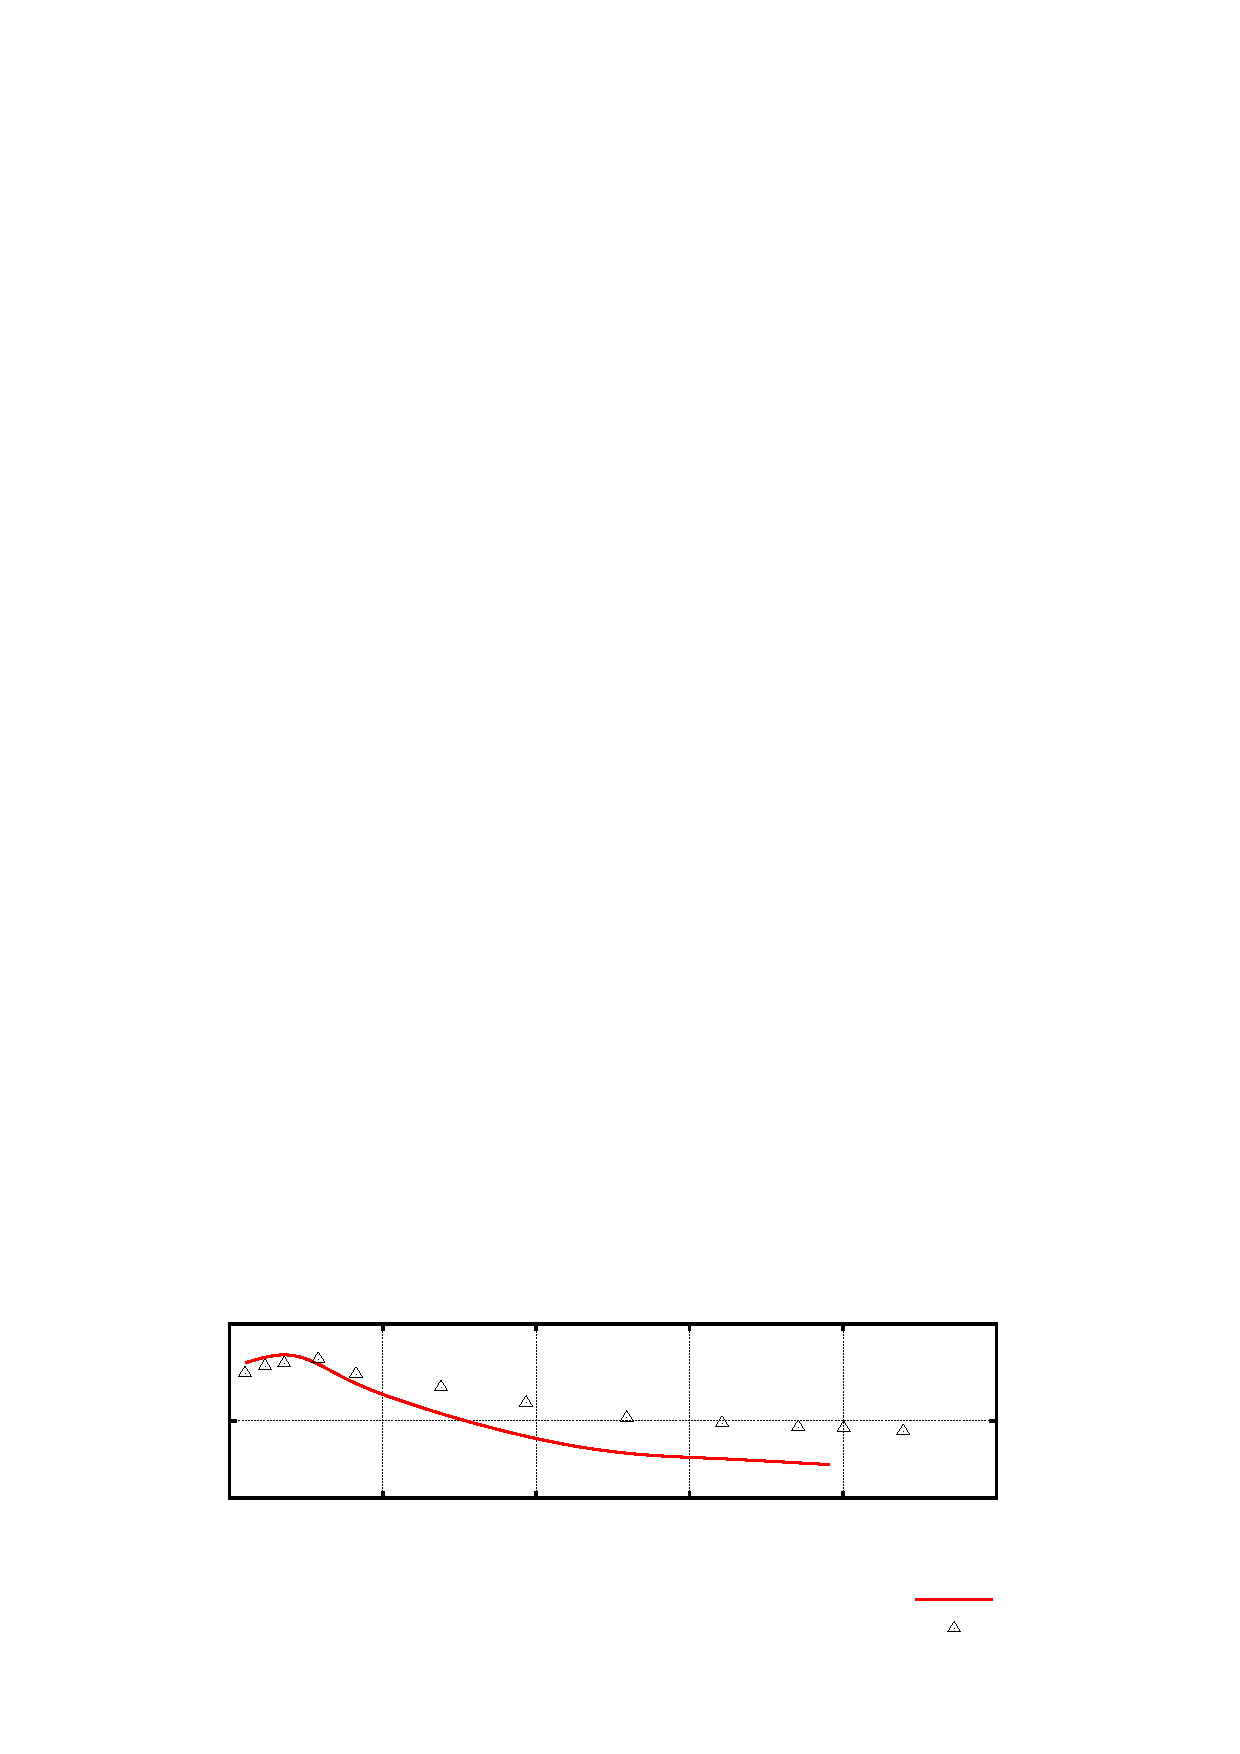
\includegraphics[width={453.50bp},height={198.40bp}]{nikitin3}}%
    \gplfronttext
  \end{picture}%
\endgroup

 	}
 	\caption{Сравнение распределений скоростей на спинке лопатки диагональной решётки и плоской \cite{Nikitin1966}} 
 	\label{fig:nikitin}
 \end{figure}
 
При рассмотрении течения во вращающейся пространственной решётке в относительной системе координат, в которой решётка остаётся неподвижной, поток является вихревым \cite{Jukovskiy1967,Viktorov1969}. Допущение о потенциальности течения в ядре потока перестаёт иметь смысл как и использование конформных отображений. Пересчёт данных продувок плоских профилей в таком случае становится неправомочным. Возможно использование теоретических характеристик, полученных, например, методами особенностей. Поток, при этом подходе, является наложением двух характерных потоков: бесциркуляционном обтекании неподвижной решётки профилей и движущейся решётки в отсутствии расхода.
 
Современные методы математического моделирования позволяют получить численное решение о вязком трёхмерном течении в проточной части рабочего колеса без использования сложных ограниченных моделей описанных выше, основываясь на более общих представлениях о законах течения. На данный момент, одним из основных подходов к созданию высокоэффективной компрессорной техники является численное трехмерное моделирование течения в проточной части, базирующееся на уравнениях Навье-Стокса, осреднённых по Рейнольдсу (CFD 3D RANS). Бурное развитие вычислительной техники в последние десятилетия и развитие универсальных программных комплексов, реализующих методы CFD 3D RANS, определило доминирующее положение этих методов в инженерных применениях. Через серии прямых задач решают задачи о проектировании турбомашин с меридиональным ускорением, обучая для этого нейронную сеть \cite{Bamberger2017}, или варьируя отдельные параметры для проектирования на конкретное задание \cite{Qiushi2010,Kim2018}. К сожалению, даже самые современные методы расчёта на высокопроизводительных вычислительных машинах не гарантируют получение решения, с достаточной точностью описывающего течение. К тому же нет общего метода моделирования течения в турбомашине. В зависимости от задачи, требуется применение различных граничных условий, моделей турбулентности и т.п. Данные полученные методами CFD 3D RANS, как и любыми другими расчётными методами, необходимо подтверждать в физическом эксперименте \cite{Michaud2016,Pandya2020}. 

\FloatBarrier
           % Глава 1
\chapter{Расчётное исследование течения в проточной части вентилятора с меридиональным ускорением потока}

Стоит сказать, что на основании главы \ref{ch:ch1}, необходимо изучить это хитрое течение подробнее

\section{Математическое моделирование течения в межлопаточном канале}

	\subsection{Конформное отображение}

Одним из наиболее эффективных подходов является конформное отображение осесимметричной поверхности тока на плоскость, как это представлено на рисунке.
Рассмотрим элементарную струйку тока, заключенную между двумя бесконечно близкими поверхностями тока, следуя допущению, что поверхности тока осесимметричны, под толщиной струи \(h\) примем расстояние между ограничивающими поверхностями. Осесимметричная поверхность описывается некоторой зависимостью радиуса от осевой координаты \(r=r(z)\) и образуется поворотом линии вокруг продольной оси \(z\).

	\subsection{Конформное отображение}
	\subsection{Потенциальное двухмерное течение в слое переменной толщины в движущейся решётке профилей}
	\subsection{Вычисление скорости жидкости}
	\subsection{Решение методом дискретных вихрей}
	\subsection{Сравнение результатов моделирований выполненных двумя методами}

\section{Повышение напора в рабочем колесе}
	\subsection{Исследуемые решётки профилей}
	\subsection{Повышение напора в рабочем колесе}
	\subsection{Сравнение результатов моделирований выполненных двумя методами}
	
\section{Влияние формы проточной части на меридиональные линии тока}
\section{Влияние вращения решётки}

\FloatBarrier
           % Глава 2
%\include{Dissertation/part3}           % Глава 3
%\include{Dissertation/conclusion}      % Заключение
\chapter*{\nomname}                         % Заголовок
\addcontentsline{toc}{chapter}{Список сокращений и условных обозначений}    % Добавляем его в оглавление
\eqexplSetIntro{}

\begin{eqexpl}
\item{\(P_\nu\)} полное давление вентилятора, \(\si\pascal\)
\item{\(P_{s\nu}\)} статическое давление вентилятора, \(\si\pascal\)
\item{\(P_{d\nu}\)} динамическое давление вентилятора, \(\si\pascal\)
\item{\(N\)} потребляемая вентилятором мощность, \(\si\watt\)
\item{\(Q\)} производительность вентилятора, $\si\meter^3/\si\second$
\item{\(\eta\)} коэффициент полезного действия 
\item{\(Re\)} число Рейнольдса
\item{\(M\)} число Маха
\item{\(b\)} хорда лопатки, $\si\meter$
\item{\(W\)} скорость потока в относительном движении, $\si\meter/\si\second$
\item{\(\nu\)} кинематическая вязкость воздуха, $\si\meter^2/\si\second$
\item{\(a_{\text{зв}}\)} скорость звука в воздухе, $\si\meter/\si\second$
\item{\(\bar{H}\)} коэффициент напора
\item{\(\bar{H}_{\text{т}}\)} коэффициент теоретического напора
\item{\(\bar{c}_{a}\)} коэффициент расхода
\item{\(U_\text{к}\)} окружная скорость периферии рабочего колеса, $\si\meter/\si\second$
\item{\(F_{\text{ом}}\)} кольцевая площадь проточной части, \(\si{\meter}^2\)
\item{\(\rho\)} плотность воздуха, \(\si{\kilogram}/\si{\meter}^3\)
\item{\(\psi\)}	коэффициент давления
\item{\(\psi_{\text{т}}\)} коэффициент теоретического давления
\item{\(\varphi_{a}\)} коэффициент осевой скорости
\item{\(\varphi\)} коэффициент производительности
\item{\(\lambda\)} коэффициент мощности
\item{\(F\)} характерная площадь, \(\si{\meter}^2\)
\item{\(D\)} диаметр рабочего колеса, \(\si\meter\)
\item{\(n\)} частота вращения, об/мин
\item{\(D\)} диаметр рабочего колеса, м
\item{\( L_w \)} мощность акустического излучения, Вт
\item{$\delta_{2}$} толщина потери импульса, м
\item{$D_\text{eq}$} фактор эквивалентной диффузорности
\item{$\beta$} угол между скоростью потока в относительном движении и осью решетки, \(\si\degree\)
\item{$\tau$} густота решетки
\item{$S$}параметр закрутки
\item{\(G_\theta\)} поток момента количества движения, \(\si\kilogram \cdot \si\meter^2/\si\second^2\)
\item{\(G_x\)} поток количества движения, \(\si\kilogram \cdot \si\meter/\si\second^2\)
\item{\(R\)} радиус сопла, \(\si\meter\)
\item{$\bar{d}$} относительный диаметр
\item{\(\Delta P\)} потери полного давления, Па
\item{$\zeta$} коэффициент потери полного давления
\item{\(\pi\)} степень повышения давления в ступени
\item{\(G\)} массовый расход, \(\si\kilogram/\si\second\)
\item{\(AVDR\)} отношение осевых плотностей тока
\item{\(m\)} коэффициент меридионального ускорения
\item{\(U\)} окружная скорость колеса, \(\si\meter/\si\second\)
\item{\(C_{u}\)} окружная компонента скорости потока, \(\si\meter/\si\second\)
\item{\(\bar{c}_{u}\)} коэффициент окружной компоненты скорости потока
\item{\(\bar{r}\)} приведённый радиус
\item{\(R_\text{к}\)} радиус рабочего колеса, \(\si\meter\)
\item{$\alpha$} угол между скоростью потока в абсолютном движении и осью решетки, \(\si\degree\)
\item{\(C_{\text{u}}\)} скорость потока в относительном движении перед лопаточным венцом на среднем радиусе, $\si\meter/\si\second$
\item{\(W_{\text{u}}\)} скорость потока в абсолютном движении перед лопаточным венцом на среднем радиусе, $\si\meter/\si\second$
\item{\(c\)}  толщина профиля, максимальное расстояние между ближайшими точками корытца и спинки, \(\si\meter\) 
\item{\(f\)} изгиб профиля, максимальное расстояние от средней линии до хорды профиля, \(\si\meter\)
\item{\(t\)} шаг решётки, расстояние между соответствующими точками соседних профилей, \(\si\meter\)
\item{\(\bar{c}\)} относительная толщина профиля 
\item{\(\bar{f}\)} относительный изгиб профиля
\item{\(\tau\)} густота решётки
\item{\(\theta_{\text{г}}\)} угол установки, \(\si\degree\) 
\item{\(\beta_\text{л}\)} углы между касательными к средней линии профиля и осью решётки в точках передней и задней кромки, \(\si\degree\)
\item{\(\upsilon\)} угол изгиба профиля, \(\si\degree\)
\item{\(i\)} угол атаки, \(\si\degree\)
\item{\(\bar{x}_f\)} относительное положение точки средней линии профиля с максимальным изгибом
\item{\(A, B\)} коэффициенты решётки профилей
\item{\(r, \phi\)} полярные координаты

\end{eqexpl}

\section*{Сокращения и индексы}
\begin{eqexpl}

\item{ВНА} входной направляющий аппарат
\item{РК, К} рабочее колесо
\item{СА} спрямляющий аппарат
\item{a} осевая компонента
\item{u} окружная компонента
\item{m} меридиональная компонента
\item{ср} величина на среднем радиусе, средняя величина
\item{0} сечение перед ВНА
\item{1} сечение перед РК
\item{2} сечение перед СА
\item{3} сечение после СА

\end{eqexpl}

\eqexplSetIntro{где}
\FloatBarrier        % Список сокращений и условных обозначений
%\include{Dissertation/dictionary}      % Словарь терминов
\include{Dissertation/references}      % Список литературы
%\include{Dissertation/lists}           % Списки таблиц и изображений (иллюстративный материал)

\setcounter{totalchapter}{\value{chapter}} % Подсчёт количества глав

%%% Настройки для приложений
\appendix
% Оформление заголовков приложений ближе к ГОСТ:
\setlength{\midchapskip}{20pt}
\renewcommand*{\afterchapternum}{\par\nobreak\vskip \midchapskip}
\renewcommand\thechapter{\Asbuk{chapter}} % Чтобы приложения русскими буквами нумеровались

%\include{Dissertation/appendix}        % Приложения

\setcounter{totalappendix}{\value{chapter}} % Подсчёт количества приложений

\end{document}
